\documentclass{article}
\usepackage{geometry,amsmath,amssymb,graphicx,bbm,theorem,xr}
\usepackage[american]{babel}
\geometry{letterpaper}

%%%%%%%%%% Start TeXmacs macros
\newcommand{\Nu}{\mathrm{N}}
\newcommand{\assign}{:=}
\newcommand{\comma}{{,}}
\newcommand{\longhookrightarrow}{{\lhook\joinrel\relbar\joinrel\rightarrow}}
\newcommand{\nequiv}{\not\equiv}
\newcommand{\nin}{\not\in}
\newcommand{\nni}{\not\ni}
\newcommand{\nobracket}{}
\newcommand{\nocomma}{}
\newcommand{\nosymbol}{}
\newcommand{\tmmathbf}[1]{\ensuremath{\boldsymbol{#1}}}
\newcommand{\tmop}[1]{\ensuremath{\operatorname{#1}}}
\newcommand{\tmtextbf}[1]{{\bfseries{#1}}}
\newcommand{\tmtextit}[1]{{\itshape{#1}}}
\newcommand{\tmtextrm}[1]{{\rmfamily{#1}}}
\newcommand{\tmtextup}[1]{{\upshape{#1}}}
\newcommand{\um}{-}
\newcommand{\upl}{+}
\newenvironment{itemizedot}{\begin{itemize} \renewcommand{\labelitemi}{$\bullet$}\renewcommand{\labelitemii}{$\bullet$}\renewcommand{\labelitemiii}{$\bullet$}\renewcommand{\labelitemiv}{$\bullet$}}{\end{itemize}}
\newenvironment{proof}{\noindent\textbf{Proof\ }}{\hspace*{\fill}$\Box$\medskip}
\newtheorem{definition}{Definition}
\numberwithin{definition}{section}
\newtheorem{lemma}{Lemma}
\numberwithin{lemma}{section}
\newtheorem{proposition}{Proposition}
\numberwithin{proposition}{section}
{\theorembodyfont{\rmfamily}\newtheorem{remark}{Remark}
\numberwithin{remark}{section}
}
%%%%%%%%%% End TeXmacs macros

\newcommand{\D}{\mathcal{D}} \newcommand{\supp}{supp}
\newcommand{\proofexplanation}[1]{(#1)}
\newcommand{\C}{{\mathbbm{C}}}\newcommand{\Z}{{\mathbbm{Z}}}
\newcommand{\Sp}{{\mathbbm{S}}} \newcommand{\R}{{\mathbbm{R}}}
\newcommand{\mybra}[1]{(#1)} \newcommand{\mysbra}[1]{\left[#1\right]}
\newcommand{\mycbra}[1]{\left\{#1\right\}}

\externaldocument{master_master1}
\externaldocument{master_master3}

\begin{document}

\title{Study of symmetry breaking operators of indefinite orthogonal groups $O( p, q)$.\\ 
II. Singular symmetry breaking operators.}
\author{T. Kobayashi, O. Leontiev}
\maketitle

{\tableofcontents}

\setcounter{section}{8}
\section{Introduction}

\subsection{Motivation and Background}

Given $G$ a Lie group and $G'$ its closed subgroup, a large amount of research
in representation theory can very roughly be said to be associated with the
problem of relating representations of $G$ with representations of $G'$. It is
interesting that this problem is ``two-sided'': that is, one can be interested
in constructing representations of $G$ starting with that of $G'$, or one can
be interested in decomposing given representation of $G$ into representations
of $G'$.

Regarding the former, the standard way of obtaining representations of $G$
from that of $G'$ is a so-called induction. In particular, if one starts with
the trivial representation of $G'$, proceeding in this way he arrives at the
representation of $G$ on $L^2 ( G / G')$. Trying to understand the latter
space, one essentially finds himself in the realm of harmonic analysis,
deriving Plancherel formulas etc. Another important special case that
attracted considerable attention is the case when one start with the trivial
representation of $G'$ and inducts to $G' \times G'$ (we see $G'$ as a
subgroup of $G' \times G'$ via the diagonal embedding). It was worked upon by
Gelfand and his students {\cite{gelfand1966generalized}} in '50s ,
Harish-Chandra {\cite{harishchandra1978harmonic}} \ in '70s, T. Oshima
{\cite{oshima1984description}}, P. Delorme {\cite{delorme1998plancherel}}, T.
Kobayashi
{\cite{kobayashi1994discrete1}},{\cite{kobayashi1998discrete2}},{\cite{kobayashi1998discrete3}}
and many others in '80s-'90s.

On the other hand, the latter problem (decomposing given
infinitely-dimensional representation $\pi$ of $G$ into representations $\tau$
of noncompact $G'$) appears to be more formidable with systematic study
beginning no earlier than in '90s. The simplest setting is that of
representation $\pi$ of $G$ decomposing as a discrete sum of irreducible
representations $\tau$ of $G'$. One is then interested in computing
multiplicities (i.e. number of times given $\tau$ appears in a sum) and this
can be done via combinatorial techniques. In general, however, infinitely
dimensional representation of $G$ \tmtextit{cannot} be decomposed into the
direct sum of irreducible representations of $G'$ and one should restrict
himself to a particularly ``nice'' settings (see {\cite{kobayashi2015program}}
for a thorough discussion). What is more, one finds himself in a situation
when he has several definitions for ``multiplicity'' and these in general are
\tmtextit{not} equal. One particularly well-behaved is $m ( \pi, \tau) \assign
\dim \tmop{Hom}_{G'} ( \pi |_{G'}, \tau)$ the dimension of $G'$-intertwining
operators or, as one sometimes calls them, \tmtextit{symmetry breaking
operators}. Finally, it \tmtextit{does not} happen in general that $\dim
\tmop{Hom}_{G'} ( \pi |_{G'}, \tau)$ are all finite, so one should further
restrict himself (see {\cite{kobayashi2014classification}} for classification
of pairs $( G, G')$ when multiplicities \tmtextit{are} always finite).

One particularly nice setting is that of $( G, G') = ( O ( p + 1, q), O ( p,
q))$. On the one hand, this setting is well-behaved in the sense that one does
not face none of the anomalies mentioned in the previous paragraph. In
particular, for $O ( n + 1, 1) \supset O ( n, 1)$ the complete classification
and explicit construction of all symmetry breaking operators between
degenerate principal series was accomplished in {\cite{kobayashi2015symmetry}}
by T. Kobayashi and B. Speh recently.

On the other hand, this setting is important to number theory (cf.
Gross-Prasad conjecture {\cite{gan2011symplectic}}, Rankin-Cohen bracket
{\cite{kobayashi2015differential1}},{\cite{kobayashi2015differential2}}),
conformal geometry (cf. Juhl conformal differential operators
{\cite{juhl2009families}}) and, of course, representation theory. Already the
special cases are very important. In particular, the latter sections of
{\cite{kobayashi2015symmetry}} contain some of the applications for $O ( n +
1, 1) \supset O ( n, 1)$ case. Another particular case $O ( 2, 2) \supset O (
2, 1)$ (see {\cite{clerc2011generalized}}) is equivalent to the problem of
finding invariant trilinear forms on representations of $\tmop{SL}_2 (
\mathbbm{R})$.

Based on the (quite general) techniques introduced in
{\cite{kobayashi2015symmetry}}, we attempt to investigate the symmetry
breaking for $( G, G') = ( O ( p + 1, q), O ( p, q))$ case.

\subsection{Main results}

Letting $p, q \geqslant 1$ and $( G, G') : = ( O ( p + 1, q + 1), O ( p, q +
1))$, the purpose of this paper is to answer the following

{\noindent}\tmtextbf{Question. }\tmtextit{For given $( \lambda, \nu) \in
\mathbbm{C}^2$ explicitly describe the vector space of $\tmop{Hom}_{G'} ( I (
\lambda), J ( \nu))$ of $G'$-intertwining operators between degenerate
principal series $I ( \lambda)$ and $J ( \nu)$ of $G$ and $G'$ respectively.
In particular, find the explicit form of a basis.}{\hspace*{\fill}}{\medskip}

{\noindent}This task is made possible by the following result, which is
essentially {\cite[thm. 3.16]{kobayashi2015symmetry}}

{\noindent}\tmtextbf{Proposition. }\tmtextit{(prop. \ref{sol:prop-sol} below)
For every $( \lambda, \nu) \in \mathbbm{C}^2$ we have $\tmop{Hom}_{G'} ( I (
\lambda), J ( \nu)) \simeq \mathcal{S} \tmop{ol} ( \mathbbm{R}^{p, q} ;
\lambda, \nu)$, where $\mathcal{S} \tmop{ol} ( \mathbbm{R}^{p, q} ; \lambda,
\nu)$ denotes the space of generalized function $F \in \mathcal{D}' (
\mathbbm{R}^{p, q})$, that:
\begin{enumerate}
  \item are homogeneous of degree $\lambda - \nu - n$;
  
  \item even on $\mathbbm{R}^{p, q}$;
  
  \item satisfy $F ( m \cdot) = F ( \cdot)$ for every $m \in O ( p, q)_{e_p}
  \assign \{ m \in O ( p, q) | m \cdot e_p = e_p \}$;
  
  \item for every $b, x_0 \in \mathbbm{R}^{p, q}$ such that $b_p = 0$ and $c_b
  ( x_0) : = 1 - 2 Q ( b, x_0) + Q ( x_0) Q ( b) \neq 0$ we have
  \begin{eqnarray}
    & | c_b ( \cdot) |^{\lambda - n} F ( \psi_b ( \cdot)) = F (\cdot)
    \hspace{1em} \tmop{near} \hspace{1em} x_0, &  \nonumber\\
    & \psi_b ( x) \assign \frac{x - Q (x) b}{c_b ( x)} . &  \nonumber
  \end{eqnarray}
\end{enumerate}}{\hspace*{\fill}}{\medskip}

{\noindent}Now, the main results of the paper are as follows:

{\noindent}\tmtextbf{Proposition. }\tmtextit{(see sec. \ref{sec:doublePGP})
Let $Q$ be $( p, q)$-quadratic form and $P, P'$ denote the maximal parabolic
subgroups of $G, G'$ respectively. Then,
\begin{enumerate}
  \item one can explicitly list the $P' \backslash G / P$ coset (see prop.
  \ref{doublePGP:prop-orbitdeco});
  
  \item pullback of $P' \backslash G / P$ cosets under the $\mathbbm{R}^{p, q}
  \simeq N_- \hookrightarrow G / P$ embedding are as follows:
  \[ \left\{ \begin{array}{ll}
       \{ x_p \neq 0, Q \neq 0 \} \sqcup \{ x_p \neq 0, Q = 0 \} \sqcup \{ x_p
       = 0, Q \neq 0 \} \sqcup \{ 0 \}, & p = 1\\
       \{ x_p \neq 0, Q \neq 0 \} \sqcup \{ x_p \neq 0, Q = 0 \} \sqcup \{ x_p
       = 0, Q \neq 0 \} \sqcup \{ x_p = 0, Q = 0 \} \backslash \{ 0 \} \sqcup
       \{ 0 \}, & p > 1
     \end{array} \right. \]
  where, say $\{ x_p \neq 0, Q \neq 0 \} \assign \{ x \in \mathbbm{R}^{p, q} |
  Q ( x) \neq 0, x_p \neq 0 \}$;
  
  \item $P' N_- P = G$.
\end{enumerate}}{\hspace*{\fill}}{\medskip}

{\noindent}\tmtextbf{Remark. }In particular, the third item supplies necessary
hypothesis for the proof of $\tmop{Hom}_{G'} ( I ( \lambda), J ( \nu)) \simeq
\mathcal{S} \tmop{ol} ( \mathbbm{R}^{p, q} ; \lambda, \nu)$ isomorphism, while
the second item implies that an element of $\mathcal{S} \tmop{ol} (
\mathbbm{R}^{p, q} ; \lambda, \nu)$ can have its support equal only to: $\{ 0
\}$, $P \assign \{ x \in \mathbbm{R}^{p, q} | x_p = 0 \}$, $C \assign \{ x \in
\mathbbm{R}^{p, q} | Q ( x) = 0 \}$, $P \cap C$, $C \cup P$ or
$\mathbbm{R}^{p, q}$.

We will therefore use the notation $\mathcal{S} \tmop{ol}_S ( \mathbbm{R}^{p,
q} ; \lambda, \nu)$ to denote elements of $\mathcal{S} \tmop{ol} (
\mathbbm{R}^{p, q} ; \lambda, \nu)$ which are supported inside some fixed
$S$.{\hspace*{\fill}}{\medskip}

{\noindent}\tmtextbf{Proposition. }\tmtextit{We have the following:
\begin{enumerate}
  \item (prop. \ref{supp-R:prop-3}) for $\lambda, \nu \in \mathbbm{C}$ with
  $\lambda - \nu \nin -\mathbbm{Z}_{\geqslant 0}$ one can extend the
  well-defined product of generalized functions
  \[ \frac{| x_p |^{\lambda + \nu - n}}{\Gamma ( ( \lambda + \nu - n + 1) /
     2)} \cdot \frac{| Q |^{- \nu}}{\Gamma ( ( 1 - \nu) / 2)} \in \mathcal{D}'
     ( \mathbbm{R}^{p, q} \backslash \{ 0 \}) \]
  to an element $K_{\lambda, \nu}^{\mathbbm{R}^n}$ of $\mathcal{S} \tmop{ol} (
  \mathbbm{R}^{p, q} ; \lambda, \nu)$. One can also explicitly determine its
  support (see prop. \ref{KR-normalization-recur:prop-supp}), which is
  generically equal to $\mathbbm{R}^{p, q}$;
  
  \item (prop. \ref{supp-Q:prop-sol-extending}) For $\nu \nin
  2\mathbbm{Z}_{\geqslant 0} + 1$ $\mathcal{S} \tmop{ol}_{\{ 0 \}} (
  \mathbbm{R}^{p, q} ; \lambda, \nu) =\mathcal{S} \tmop{ol}_C (
  \mathbbm{R}^{p, q} ; \lambda, \nu)$, while for $\nu \in
  2\mathbbm{Z}_{\geqslant 0} + 1$ fixed and $\lambda \in \{ \lambda \in
  \mathbbm{C} | \lambda - \nu \in -\mathbbm{Z}_{\geqslant 0} \}$ one can
  extend the well-defined product of generalized functions
  \[ \left\{ \begin{array}{ll}
       \delta^{( \nu - 1)} ( Q) \cdot | x_p |^{\lambda + \nu - n}, & p = 1\\
       \delta^{( \nu - 1)} ( Q) \cdot \frac{| x_p |^{\lambda + \nu -
       n}}{\Gamma ( ( \lambda + \nu - n + 1) / 2)}, & p > 1
     \end{array} \right. \]
  to an element $K_{\lambda, \nu}^C$ of $\mathcal{S} \tmop{ol}_C (
  \mathbbm{R}^{p, q} ; \lambda, \nu) \backslash\mathcal{S} \tmop{ol}_{\{ 0 \}}
  ( \mathbbm{R}^{p, q} ; \lambda, \nu)$. One can also explicitly determine its
  support (see prop. \ref{supp-Q:prop-supp-xnoq0}), which is generically equal
  to $C$;
  
  \item (sec. \ref{sec:supp-P}) For $\lambda + \nu - n = - 1 - 2 k, \; k \in
  \mathbbm{Z}_{\geqslant 0}$ the distribution
  \begin{eqnarray}
    & K^P_{\lambda, \nu} \assign \sum_{i = 0}^k \frac{(- 1)^i (2 k) !
    (\nu)^{}_i}{(2 k - 2 i) !i!} \delta^{(2 k - 2 i)} (x_p) \otimes
    \tilde{Q}_i \in \mathcal{D}' ( \mathbbm{R}^{p, q} ; \lambda, \nu), & 
    \nonumber\\
    & (\nu)^{}_i \assign \nu (\nu + 1) \ldots (\nu + i - 1), &  \nonumber\\
    & \tilde{Q}_i \assign \left\{ \begin{array}{ll}
      \tilde{Q}_+^{- \nu - i} + \tilde{Q}_-^{- \nu - i}, & i \in 2 \Z_{\ge 0},
      p \geqslant 2\\
      \tilde{Q}_+^{- \nu - i} - \tilde{Q}_-^{- \nu - i}, & i \in 2 \Z_{\ge 0}
      + 1, p \geqslant 2\\
      | \tilde{Q} |^{- \nu - i}, & i \in 2 \Z_{\ge 0}, p = 1\\
      - | \tilde{Q} |^{- \nu - i}, & i \in 2 \Z_{\ge 0} + 1, p = 1
    \end{array} \right. &  \nonumber
  \end{eqnarray}
  (with $\tilde{Q}$ being $( p - 1, q)$-quadratic form) is an element of
  $\mathcal{S} \tmop{ol}_P ( \mathbbm{R}^{p, q} ; \lambda, \nu)$ well-defined
  for $\nu \in \mathbbm{C}$ outside some discrete subset. Again, support is
  generically equal to $P$ and can be explicitly determined (see sec.
  \ref{sec:KP-normalization}).
\end{enumerate}}{\hspace*{\fill}}{\medskip}

{\noindent}\tmtextbf{Remark. }Three families $K_{\lambda,
\nu}^{\mathbbm{R}^n}$, $K_{\lambda, \nu}^C$ and $K_{\lambda, \nu}^P$ are thus
constructed for parameters outside some codimension one subsets of
$\mathbbm{C}^2$, $\mathbbm{C}$ and $\mathbbm{C}$ respectively. It turns out
that they have poles at these subsets, hence in order to extend these families
to the whole $\mathbbm{C}^2$, $\mathbbm{C}$ and $\mathbbm{C}$ respectively,
one should ``normalize'' them, that is, divide by some meromorphic function in
order to eliminate poles. This situation is much similar to the way one
normalizes generalized function $x_+^{\lambda}$ to show that $x_+^{\lambda} /
\Gamma ( \lambda + 1)$ is holomorphic (see {\cite[sec.
1.3.5]{gelfand1980distribution}}).{\hspace*{\fill}}{\medskip}

{\noindent}\tmtextbf{Proposition. }\tmtextit{We have the following:
\begin{enumerate}
  \item (sec. \ref{sec:KC-normalization}) Depending on $p, q \in
  \mathbbm{Z}_{\geqslant 1}$ and $\nu \in 2\mathbbm{Z}_{\geqslant 0} + 1$, one
  can find meromorphic function $N$ so that $K_{\lambda, \nu}^C / N$
  holomorphically extends to all $\lambda \in \mathbbm{C}$ to give a nonzero
  element of $\mathcal{S} \tmop{ol}_C ( \mathbbm{R}^{p, q} ; \lambda, \nu)$.
  Its support is explicitly determined.
  
  \item (sec. \ref{sec:KP-normalization}) Depending on $p, q \in
  \mathbbm{Z}_{\geqslant 1}$ and $k \assign - ( \lambda + \nu - n + 1) / 2$,
  one can find meromorphic function $N$ so that $K_{\lambda, \nu}^P / N$
  holomorphically extends to all $\nu \in \mathbbm{C}$ ($\lambda$ is
  determined by $\nu$ subject to $\lambda + \nu - n = - 1 - 2 k$ condition) to
  give a nonzero element of $\mathcal{S} \tmop{ol}_P ( \mathbbm{R}^{p, q} ;
  \lambda, \nu)$. Its support is explicitly determined.
  
  \item (sec. \ref{sec:KR-normalization-even}) For $q \in 2\mathbbm{Z}$ and
  depending on $p, q \in \mathbbm{Z}_{\geqslant 1}$, one can find meromorphic
  function $N$ so that $K_{\lambda, \nu}^{\mathbbm{R}^n} / N$ holomorphically
  extends to all $ ( \lambda, \nu) \in \mathbbm{C}^2$ to give an element of
  $\mathcal{S} \tmop{ol}_{} ( \mathbbm{R}^{p, q} ; \lambda, \nu)$ which is
  nonzero outside the discrete subset of $\mathbbm{C}^2$.
\end{enumerate}}{\hspace*{\fill}}{\medskip}

\subsection{Organization of the paper}

Following the style of {\cite{kobayashi2015symmetry}} it was attempted to make
the exposition detailed, elementary and as self-contained as possible.
Regarding the latter, the effort was made to clearly state all the statements
that we use without proof as ``facts'' and give clear references. The notable
exception to this are the statements from {\cite{kobayashi2015symmetry}}: we
use these within our proofs, still, hopefully, with clear indication of which
statements and where were used.

Now, the remaining sections are organized as follows:
\begin{itemizedot}
  \item in sections \ref{sec:holomorphicity-preserving} to
  \ref{sec:pull-tensor-mult} miscellaneous results are collected. These will
  be used in latter sections, mostly in and after the section \ref{sec:lem67};
  they are independent of other sections and (largely) of each other; we
  suggest to omit them on the first reading and return to them later as
  necessary;
  
  \item in section \ref{sec:def-n-nots} objects that we are dealing with are
  defined (the most importantly, groups $G \supset G'$ and their degenerate
  principal series $I ( \lambda)$ and $J ( \nu)$ respectively), the main goal
  of the paper is also stated;
  
  \item in section \ref{sec:doublePGP} two crucial results are stated and
  proven. Of these the first one is that $P' N_- P = G$ equality holds. It
  provides necessary hypothesis to apply {\cite[thm
  3.16]{kobayashi2015symmetry}} which sets up the isomorphism \
  $\tmop{Hom}_{G'} ( I ( \lambda), J ( \nu)) \simeq \mathcal{S} \tmop{ol} (
  \mathbbm{R}^{p, q} ; \lambda, \nu)$. The second one is the description of
  $P' \backslash G / P$ double coset space and description of pullback of
  these cosets under the $N_- \hookrightarrow G / P$ embedding. It allows us
  to predict what supports elements of $\mathcal{S} \tmop{ol} (
  \mathbbm{R}^{p, q} ; \lambda, \nu)$ may have;
  
  \item in section \ref{sec:sol} $\mathcal{S} \tmop{ol} ( \mathbbm{R}^{p, q} ;
  \lambda, \nu)$ is formally defined and it is shown to be isomorphic with the
  space of SBOs $\tmop{Hom}_{G'} ( I ( \lambda), J ( \nu))$ for every fixed
  pair of parameters $( \lambda \comma \nu) \in \mathbbm{C}^2$;
  
  \item in section \ref{sec:n-nonequiv} a counter-example related to the
  notions introduced in section \ref{sec:sol} is constructed; it can be
  omitted without the loss of continuity;
  
  \item in \ref{sec:lem67} system of equations that define $\mathcal{S}
  \tmop{ol} ( \mathbbm{R}^{p, q} ; \lambda, \nu)$ is explicitly solved, but on
  a smaller set $\{ x \in \mathbbm{R}^{p, q} | Q ( x) \neq 0 \}$ (where $Q$ is
  a $( p, q)$-quadratic form);
  
  \item in sections \ref{sec:supp-R}, \ref{sec:supp-P} and \ref{sec:supp-Q}
  elements of $\mathcal{S} \tmop{ol} ( \mathbbm{R}^{p, q} ; \lambda, \nu)$ are
  constructed, that are supported within $\mathbbm{R}^{p, q}$, $\{ x \in
  \mathbbm{R}^{p, q} | x_p = 0 \}$ and $\{ x \in \mathbbm{R}^{p, q} | Q ( x) =
  0 \}$ respectively for $( \lambda, \nu)$ lying in some open subsets of
  $\mathbbm{C}^2$ (different for all three cases). These elements are
  constructed, so that they depend on $( \lambda, \nu)$ holomorphically;
  
  \item in section \ref{sec:diffSBO} for all $( \lambda, \nu) \in
  \mathbbm{C}^2$ elements of $\mathcal{S} \tmop{ol} ( \mathbbm{R}^{p, q} ;
  \lambda, \nu)$ that are supported within $\{ 0 \}$ are classified; these
  correspond to differential SBO under the correspondence $\tmop{Hom}_{G'} ( I
  ( \lambda), J ( \nu)) \simeq \mathcal{S} \tmop{ol} ( \mathbbm{R}^{p, q} ;
  \lambda, \nu)$;
  
  \item in section \ref{sec:k-finite} a method to analytically continuate
  families of elements of $\mathcal{S} \tmop{ol} ( \mathbbm{R}^{p, q} ;
  \lambda, \nu)$ to a larger parameter sets is introduced;
  
  \item in sections \ref{sec:KC-normalization}, \ref{sec:KP-normalization} and
  \ref{sec:KR-normalization-even} definitions of $K_{\lambda, \nu}^C$,
  $K_{\lambda, \nu}^P$ and $K_{\lambda, \nu}^{\mathbbm{R}^n}$ made in sections
  \ref{sec:supp-Q}, \ref{sec:supp-P} and \ref{sec:supp-R} respectively are
  extended to all parameters $( \lambda, \nu) \in \mathbbm{C}^2$, so that
  holomorphic dependence is preserved. For $K_{\lambda, \nu}^{\mathbbm{R}^n}$
  this is done under the assumption $q \in 2\mathbbm{Z}$;
  
  \item section \ref{sec:knappstein} is an application of techniques
  introduced in {\cite{kobayashi2015symmetry}} and used in this paper, to the
  problem of finding a concrete form of $G$-invariant $I ( \lambda)
  \rightarrow I ( n - \lambda)$ operator in a relatively elementary and
  straightforward way; the obtained results parallel some of that of
  {\cite{KO1}}.
\end{itemizedot}
Starting from section \ref{sec:doublePGP} all sections have the same
structure: first, every section opens with a brief introduction. Next, three
subsections follow. The first one, ``Main results'' contains the statements of
main propositions and definitions this section contains. Next, subsection
``Auxiliary lemmas'' follow, containing stated and immediately proven lemmas
that we use to prove the main results of the section. Finally, in the
subsection ``Proofs'' main results of the section are proven.

\subsection{Acknowledgments}

I'd like to thank my supervisor Toshiyuki Kobayashi who brought this topic to
my attention and taught me all the techniques necessary.

\section{$\mathcal{S} \tmop{ol}_{} ( U ; \lambda, \nu)$ and related
notions}\label{sec:sol}

\subsection{Main results}

\begin{definition}
  \label{def-n-nots:def-n+invar}For $F \in \D' (U)$, where $U \subset
  \mathbbm{R}^{p, q}$ is an open set, we say that $F$ is
  \tmtextbf{$N_+'$-invariant on $U$} if $\forall b \in \mathbbm{R}^{p, q}$
  with $b_p = 0$ and $x_0 \in U$ such that $\frac{x_0 - Q (x_0) b}{1 - 2 Q
  (x_0, b) + Q (x_0) Q (b)} \in U$ and the expression makes sense (i.e. the
  denominator is non-zero) we have
  \begin{equation}
    \label{eq-Nequiv} | 1 - 2 Q (b, x) + Q (x) Q (b) |^{\lambda - n} F \left(
    \frac{x - Q (x) b}{1 - 2 Q (x, b) + Q (x) Q (b)} \right) = F (x)
  \end{equation}
  equality holding for $x$ near $x_0$.
\end{definition}

\begin{definition}
  \label{sol:def-sol}For $F \in \D' (U)$, where $U \subset \mathbbm{R}^{p, q}$
  is the open set, we say that $F \in \mathcal{S} \tmop{ol} (U ; \lambda,
  \nu)$ if the following holds:
  \begin{enumerate}
    \item if $x_0 \in U$ and $- x_0 \in U$, then $F (x) = F (- x)$ for $x$
    near $x_0$;
    
    \item if $(m, x_0, m \cdot x_0) \in O (p, q)_{e_p} \times U \times U$,
    then $F (x) = F (m \cdot x)$ for $x$ near $x_0$, where $O (p, q)_{e_p}
    \assign \{g \in O (p, q) |g \cdot e_p = e_p \}$;
    
    \item if $(\alpha, x_0, \alpha x_0) \in \mathbbm{R}_{> 0} \times U \times
    U$, then $\alpha^{\lambda - \nu - n} F (x) = F (\alpha x)$ for $x$ near
    $x_0$;
    
    \item $F$ is $N_+'$-invariant on $U$.{
    
    }{
    
    }For a closed set $S \subset U$ we will also use the notation $\mathcal{S}
    \tmop{ol}_S ( U ; \lambda, \nu) \assign \{ u \in \mathcal{S} \tmop{ol} ( U
    ; \lambda, \nu) | \tmop{supp} ( u) \subset S \}$
  \end{enumerate}
\end{definition}

\begin{remark}
  It is easy to observe the following:
  \begin{enumerate}
    \item more precisely, item 1. means that for $( x_0, - x_0) \in U^2$ there
    is an open sets $U \supset V \ni x_0$ such that for $\psi : x \mapsto - x$
    a difeomorphism of $\mathbbm{R}^{p, q}$ we have $u |_V = \psi^{\ast} ( u
    |_{\psi ( V)})$. Similarly, items 2, 3 and $N_+'$-invariance are
    explained. Note that all condinitions of definition \ref{sol:def-sol} are
    particular instances of situation in lemma \ref{sol:lem-holodep} (say, for
    item 4 one takes $\psi = \psi_b$ and $f = | c_b |$);
    
    \item that if $U = \bigcup_{i \in \Lambda} U_i$ is an open cover, then for
    $u \in \mathcal{D}' ( U)$ and $( \lambda, \nu) \in \mathbbm{C}^2$ we have
    $u \in \mathcal{S} \tmop{ol} ( U ; \lambda, \nu) \Leftrightarrow \forall i
    \in \Lambda, \; u |_{U_i} \in \mathcal{S} \tmop{ol} ( U_i ; \lambda,
    \nu)$;
    
    \item When $U$ is an open cone, item 3 is equivalent to the usual
    definition of homogeneity of order $\lambda - \nu - n$;
  \end{enumerate}
\end{remark}

\begin{proposition}
  \label{sol:prop-sol}For every $( \lambda, \nu) \in \mathbbm{C}^2$ we have
  $\mathcal{S} \tmop{ol} ( \mathbbm{R}^{p, q} ; \lambda, \nu) \simeq
  \tmop{Hom}_{G'} ( I ( \lambda), J ( \nu))$.
\end{proposition}

\begin{proposition}
  \label{sol:prop-holocont}Suppose that $\Omega' \subseteq \Omega \subset
  \mathbbm{C}^k$ are open sets and $\Omega \ni \mu \mapsto ( \lambda ( \mu),
  \nu ( \mu)) \in \mathbbm{C}^2$ is holomorphic open map. Suppose further that
  $K_{\mu} \in \mathcal{D}' ( U)$ with ($U \subset \mathbbm{R}^{p, q}$:open)
  holomorphically depends on $\mu \in \Omega$ and for $\mu \in \Omega'$ we
  have $K_{\mu} \in \mathcal{S} \tmop{ol} ( U ; \lambda ( \mu), \nu ( \mu))$.
  Then $K_{\mu} \in \mathcal{S} \tmop{ol} ( U ; \lambda ( \mu), \nu ( \mu))$
  for $\mu \in \Omega$ as well.
\end{proposition}

\begin{remark}
  The last two propositions are \tmtextbf{not} new. The statement and proof
  below are just rephrasing and somehow elaboration of those given in
  {\cite[thm 3.16]{kobayashi2015symmetry}} and {\cite[prop.
  3.18]{kobayashi2015symmetry}} respectively.
\end{remark}

\subsection{Auxiliary lemmas}

\begin{lemma}
  \label{sol:lem-unfold}For $G \assign O ( p + 1, q + 1)$ and $\lambda \in
  \mathfrak{a}_{\mathbbm{C}}^{\ast}$ let $\lambda : P \rightarrow
  \mathbbm{C}^{\times}$ be a homomorphism defined as in proposition
  \ref{def-n-nots:prop-degseries}. Then for $C^{\infty} ( G)_{\lambda} \assign
  \left\{ f \in C^{\infty} ( G) | \forall p \in P, \; f ( \cdot p) = \lambda (
  p^{- 1}) f ( \cdot) \right\}$ we have the map $C^{\infty} \ni f ( \cdot)
  \mapsto [ g P \mapsto [ g, f ( g)]] \in C^{\infty} ( G \times_P
  \mathbbm{C}_{\lambda})$ being an isomorphism of vector spaces.
\end{lemma}

\begin{proof}
  The well-definedness of this map is straightforward to verify. Conversely,
  given $f' \in C^{\infty} ( G \times_P \mathbbm{C}_{\lambda})$, we can
  construct the corresponding element of $C^{\infty} ( G)_{\lambda}$ as
  follows: for $g \in G$ we let $f ( g) \assign x \in \mathbbm{C}$ such that
  $( g, x) \in f' ( g H)$. It is easy to see that such $x$ exists and is
  unique. The obtained mapping $g \mapsto f ( g)$ forms a smooth map of
  $C^{\infty} ( G)$, which is in fact an element of $C^{\infty} (
  G)_{\lambda}$, as we should have $g p$ for $p \in P$ being mapped to
  $\lambda ( p^{- 1}) f ( g)$, since $[ g, x] = [ g p, \lambda ( p^{- 1}) x]$.
\end{proof}

\begin{lemma}
  \label{sol:lem-commdiag}Recall the $G \assign O ( p + 1, q + 1)
  \curvearrowright \Xi$ action. Fix $U \subset N_- \simeq \mathfrak{n}_-
  \simeq \mathbbm{R}^{p, q}$ an open set. The following diagram then commutes:
  
  \begin{center}
    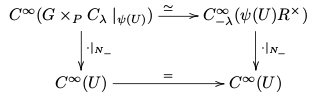
\includegraphics[scale=0.6]{master_master-6.png}
  \end{center}
  
  Here for $\lambda \in \mathbbm{C}$, and $V \subset \Xi$ invariant under
  multiplication by $\mathbbm{R}^{\times}$ we let $C^{\infty}_{- \lambda} ( V)
  \assign \left\{ f \in C^{\infty} ( V) | \forall \alpha \in
  \mathbbm{R}^{\times}, \; f ( \alpha \cdot) = | \alpha |^{- \lambda} f (
  \cdot) \right\}$. $G \times_P \mathbbm{C}_{\lambda} |_{\psi ( U)}$ denotes
  the portion of vector bundle $G \times_P \mathbbm{C}_{\lambda}$ above $\psi
  ( U)$. $\psi ( \cdot)$ denotes embedding of $N_- \simeq \mathfrak{n}_-
  \simeq \mathbbm{R}^{p, q}$ into $G / P$ (on the left) or into $\Xi$ (on
  right) The top map is a continuous $G$-equivariant isomorphism, defined for
  $f ( \cdot) \in C^{\infty} ( G \times_P \mathbbm{C}_{\lambda}) \simeq
  C^{\infty} ( G)_{\lambda}$ as $\tilde{f} \in C^{\infty}_{- \lambda} ( \Xi)$,
  $\tilde{f} ( g p_+) \assign f ( g)$ (here $p_+ \assign ( 1, 0_{p + q}, 1)
  \in \Xi$). The left vertical arrow is a restriction to an open subset $\psi
  ( U) P \subset G / P$. The right-vertical arrow is restriction to a
  submanifold $U \cdot ( 1, 0_{p + q}, 1) \subset \Xi$.
\end{lemma}

\begin{proof}
  We assume $U =\mathfrak{n}_-$ for simplicity, the proof for general $U$
  proceeds in precisely the same manner. First, we show that for smooth
  functions the top map is well-defined. Indeed, let $f \in C^{\infty} (
  G)_{\lambda} $ as in lemma \ref{sol:lem-unfold}. Then the map $\tilde{f} : g
  ( 1, 0_{p + q}, 1) \mapsto f ( g)$ on $G p_+$ is well-defined, as
  centralizer of $p_+$ equals to $M^0 N_+$ by proposition
  \ref{def-n-nots:prop-ximodel}, and for $\lambda : P \rightarrow
  \mathbbm{C}^{\times}$ is in lemma \ref{sol:lem-unfold}, we have $\lambda (
  M^0 N_+)$. Moreover, as action $G \curvearrowright \Xi$ is transitive by an
  argument similar to that of lemma \ref{doublePGP:lem-Gp-act-Xi}, we have $g
  p_+ \mapsto f ( g)$ being well-defined map $\tilde{f} \in C^{\infty} (
  \Xi)$.
  
  We next show that $\tilde{f}$ is also homogeneous of degree $- \lambda$, as
  we have for $\tilde{f} ( - g p_+) = \tilde{f} ( g m_0 p_+)$, for $m_0
  \assign \tmop{diag} ( - 1, 1_{p + q}, 1) \in M$ and hence $\tilde{f} ( g m_0
  p_+) \assign f ( g m_0) = f ( g_{}) = \tilde{f} ( g p_+)$, since $f \in
  C^{\infty} ( G)_{\lambda}$. Similarly, for $\alpha \in \mathbbm{R}_{> 0}$ we
  have $\tilde{f} ( \alpha g p_+) = \tilde{f} ( g a ( t) p_+)$ with $a ( t)$
  is in (\ref{def-n-nots:eq-A}) for $t = \ln ( \alpha)$, and hence the chain
  of equalities continues as $= \tilde{f} ( g a ( t) p_+) \assign f ( g a (
  t)) = e^{- \lambda t} f ( g) = \alpha^{- \lambda} f ( g p_+)$. This shows
  homogeneity.
  
  The fact that top map is isomorphic is implied by the fact that we can
  construct inverse map $C^{\infty}_{- \lambda} ( \Xi) \rightarrow C^{\infty}
  ( G)_{\lambda}$ by $\tilde{f} \mapsto f$, where we set $f ( g) \assign
  \tilde{f} ( g p_+)$. It can be similarly to above shown that this map is
  well-defined.
  
  Finally, the diagram commutes by direct inspection and proposition
  \ref{def-n-nots:prop-ximodel}.
\end{proof}

\begin{lemma}
  \label{sol:lem-holodep}Suppose $\Omega' \subset \Omega \subset
  \mathbbm{C}^m$ are an open set and $\kappa : \Omega \rightarrow \mathbbm{C}$
  is holomorphic. Suppose also that $U, V \subset \mathbbm{R}^k$ are open with
  $\psi : U \rightarrow V$ diffeomorphism, and $K_{\mu}^U \in \mathcal{D}' (
  U), K^V_{\mu} \in \mathcal{D}' ( V)$ are holomorphic in $\mu \in \Omega$.
  Then if for $f \in C^{\infty} ( U \rightarrow \mathbbm{R}_{> 0})$ we have
  $\forall \mu \in \Omega', \; f^{\kappa ( \mu)} K^U_{\mu} = \psi^{\ast}
  K^V_{\mu}$, then this also holds for every $\mu \in \Omega$.
\end{lemma}

\begin{proof}
  In the light of holomorphic rigidity, it suffices to show that $\psi^{\ast}
  K^V_{\mu}, f^{\kappa ( \mu)} K^U_{\mu} \in \mathcal{D}' ( U)$ are
  holomorphic in $\mu \in \Omega$. For $\psi^{\ast} K_{\mu}^V$ this is readily
  given by proposition \ref{holomorphicity-preserving:prop-pullback-holo}.
  Regarding $f^{\kappa ( \mu)} K^U_{\mu}$, lemma
  \ref{KR-normalization-recur:lem-mult-smth} implies that the latter can be
  seen as product of distributions and hence in the light of propositions
  \ref{holomorphicity-preserving:prop-tensor-holo} and
  \ref{holomorphicity-preserving:prop-pullback-holo}, it suffices to show that
  $f^{\kappa ( \mu)}$ is holomorphic when seen as an element of $\mathcal{D}'
  ( U)$. This can be proven directly.
\end{proof}

\subsection{Proofs}

\begin{definition}
  \label{sol:def-localaciton}For $\lambda \in \mathbbm{C}$ let $P'
  \curvearrowright G / P$ by left multiplication. Introduce also an embedding
  $\mathbbm{R}^{p, q} \ni w \mapsto \psi ( w) \assign n_- ( w) P \in G / P$.
  Suppose now that $( U, V)$ is a pair of open subsets of $\mathbbm{R}^{p, q}$
  and $p' \in P$ such that $\psi ( U) = p' \psi ( V)$. Then straightforward
  generalization of lemma \ref{KR-normalization-recur:lem-pull-comm-restr}
  tells us that the following diagram commutes
  \begin{center}
    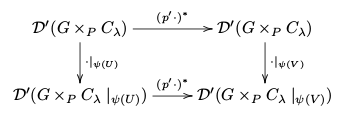
\includegraphics[scale=0.6]{master_master-7.png}
  \end{center}
  here $G \times_P \mathbbm{C}_{\lambda} |_{\psi ( U)}$ denotes portion of the
  bundle above $\psi ( U)$ and similarly for $\psi ( V)$. The top and bottom
  maps are isomorphisms. Now, pullback by $\psi ( \cdot)$ induces the
  isomorphism $\mathcal{D}' ( U) \rightarrow \mathcal{D}' ( V)$ so that the
  following map commutes:
  
  \begin{center}
    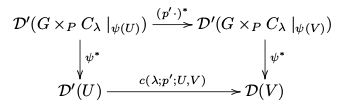
\includegraphics[scale=0.6]{master_master-8.png}
  \end{center}
  
  all maps of it are isomorphisms and we will call the one at the bottom by $c
  ( \lambda ; p' ; U, V) : \mathcal{D}' ( U) \rightarrow \mathcal{D}' ( V)$.
\end{definition}

\begin{definition}
  \label{sol:def-D'n}For $( \lambda, \nu) \in \mathbbm{C}^2$ we let
  $\mathcal{D}' ( \mathfrak{n}_-, \mathbbm{C}_{n - \lambda} \otimes
  \mathbbm{C}_{\nu})^{M' A', \mathfrak{n}'_+}$ to denote the space of $u \in
  \mathcal{D}' ( \mathbbm{R}^{p, q})$ such that for all $U, V, p'$ as in
  definition \ref{sol:def-localaciton} we have $u |_V = \nu^{} ( ( p')^{- 1})
  c ( n - \lambda ; p' ; U, V) u |_V$ with homomorphism $\nu : P' \rightarrow
  \mathbbm{C}^{\times}$ defined as in proposition
  \ref{def-n-nots:prop-degseries}.
\end{definition}

\begin{proof}
  (of prop. \ref{sol:prop-sol}) Proposition \ref{doublePGP:prop-pnp} implies
  that we can apply {\cite[thm. 3.16]{kobayashi2015symmetry}} and it
  immediately gives
  \[ \tmop{Hom}_{G'} ( I ( \lambda), J ( \nu)) \simeq \mathcal{D}' (
     \mathfrak{n}_-, \mathbbm{C}_{n - \lambda} \otimes \mathbbm{C}_{\nu})^{M'
     A', \mathfrak{n}'_+} \]
  Hence it suffices to show that $\mathcal{D}' ( \mathfrak{n}_-,
  \mathbbm{C}_{n - \lambda} \otimes \mathbbm{C}_{\nu})^{M' A',
  \mathfrak{n}'_+} =\mathcal{S} \tmop{ol} ( \mathbbm{R}^{p, q} ; \lambda,
  \nu)$ as in definition \ref{sol:def-sol}. Hence, we just need to concretely
  write down the $c ( \lambda ; p' ; U, V)$ map of \ref{sol:def-localaciton}.
  Moreover, as we have all arrows in commutative diagrams of definitions
  \ref{sol:def-localaciton} being continuous and mapping smooth to smooth,
  using approximation by smooth sections, we can assume that we have
  $\mathcal{D}'$ replaced by $C^{\infty}$ in all diagrams of definitions
  \ref{sol:def-localaciton}. Now, lemma \ref{sol:lem-commdiag} allows us to
  rewrite second commutative diagram of definition \ref{sol:def-localaciton}
  (with $\lambda$ replaced by $n - \lambda$, according to definition
  \ref{sol:def-D'n})
  
  \begin{center}
    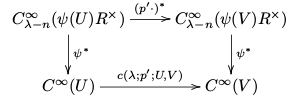
\includegraphics[scale=0.6]{master_master-9.png}
  \end{center}
  
  with an embedding $\psi : \mathbbm{R}^{p, q} \ni w \mapsto n_- ( w) \cdot (
  1, 0_{p + q}, 1) = ( 1 - Q ( w), 2 w, 1 + Q ( w)) \in \Xi$.
  
  Now, let $( p, U, V)$ be as in definition \ref{sol:def-localaciton}. If $p$
  is of the form
  \[ p \assign \left[ \begin{array}{ccc}
       1 & 0 & 0\\
       0 & m & 0\\
       0 & 0 & 1
     \end{array} \right] \in M' \]
  with $m \in O ( p, q)$ such that $m \cdot e_p = e_p$, then for $w \in
  \mathbbm{R}^{p, q}$ we have $p \cdot \psi ( w) = \psi ( m \cdot w)$.
  
  This implies that for $p, U, V$ as in definition \ref{sol:def-localaciton}
  with $p$ as above we should have $U = w V$ (and conversely all such triples
  satisfy definition \ref{sol:def-localaciton}) and $c ( p ; \lambda ; U, V) (
  F) ( \cdot) = F ( w \cdot)$.
  
  Next ,for an element $p \assign \tmop{diag} ( - 1, 1_{p + q}, - 1) \in M'$
  we have $p \cdot \psi ( w) = \psi ( - w)$. This implies that for $p, U, V$
  as in definition \ref{sol:def-localaciton} with $p$ as above we should have
  $U = - V$ (and conversely all such triples satisfy definition
  \ref{sol:def-localaciton}) and $c ( p ; \lambda ; U, V) ( F) ( \cdot) = F (
  ( - 1) \cdot)$.
  
  Next, for an element $a ( t) \in A'$ as in (\ref{def-n-nots:eq-A}), direct
  calculations show that we have we have $a ( t) \cdot \psi ( w) = e^t \psi (
  e^{- t} w)$ and hence for an element $f \in C^{\infty}_{\lambda - n}$ we
  would have $f ( a ( t) \psi ( w)) = e^{( \lambda - n) t} f ( \psi ( e^{- t}
  w))$, which implies that for $p, U, V$ as in definition
  \ref{sol:def-localaciton} with $p = a ( t)$ as above we should have $U =
  e^{- t} V$ (and conversely all such triples satisfy definition
  \ref{sol:def-localaciton}) and $c ( a ( t) ; \lambda ; U, V) ( F) ( \cdot) =
  e^{( \lambda - n) t} F ( e^{- t} \cdot)$.
  
  Finally, for $w \in \mathbbm{R}^{p, q}$ with $w_p = 0$ and an element $n_+ (
  w) \in N'_+$ as in (\ref{def-n-nots:eq-N+}), we observe that for $v \in
  \mathbbm{R}^{p, q}$ we have for $\psi_w ( \cdot)$ and $c_w ( \cdot)$ as in
  definition \ref{def-n-nots:def-n+invar}
  \[ n_+ ( w) n_- ( v) = c_w ( v) \cdot n_- ( \psi_w ( v)) \]
  whenever both sides make sense. Hence, for $p, U, V$ as in definition
  \ref{sol:def-localaciton} with $p = n_+ ( w)$ as above we should have $U =
  \psi_w ( V)$ (and conversely all such triples satisfy definition
  \ref{sol:def-localaciton}) and $c ( n_+ ( w) ; \lambda ; U, V) ( F) ( \cdot)
  = | c_w ( \cdot) |^{\lambda - n} F ( \psi_w ( \cdot))$.
  
  As the reasoning above tells us how $c ( \lambda ; p' ; U, V)$ are written
  for $p' \in M', A', N_+'$, we see that these are precisely equivalent to
  items of definition \ref{sol:def-sol} and thus Langlands decomposition of
  $P'$ tells us now that $\mathcal{D}' ( \mathfrak{n}_-, \mathbbm{C}_{n -
  \lambda} \otimes \mathbbm{C}_{\nu})^{M' A', \mathfrak{n}'_+} =\mathcal{S}
  \tmop{ol} ( \mathbbm{R}^{p, q} ; U, V)$.
\end{proof}

\begin{proof}
  (of prop. \ref{sol:prop-holocont}) In the light of the first item of remark
  after the definition \ref{sol:def-sol}, the conclusion is implied by lemma
  \ref{sol:lem-holodep}.
\end{proof}

\section{Non-equivalence of $N_+'$-invariance and
$\mathfrak{n}'_+$-invariance}\label{sec:n-nonequiv}

One might wonder whether it is possible to replace the item 4 of definition
\ref{sol:def-sol} with the differential of that (local) action of $N_+'$ on
$\mathbbm{R}^{p, q}$. We will call the latter $\mathfrak{n}_+'$-invariance.
Explicitly written, it becomes the system of differential equations
\begin{equation}
  \left[ (\lambda - n) \varepsilon_j x_j - \varepsilon_j x_j E + \frac{1}{2} Q
  (x) \frac{\partial}{\partial x_j} \right] F = 0, \hspace{1em} j = \{ 1, 2,
  \ldots, n \} \backslash \{ p \} \label{Ndiff}
\end{equation}
with $E \assign \sum_j x_j  \frac{\partial}{\partial x_j}$ and $\varepsilon_j
= + 1$ for $1 \leq j \leq p$ and $= - 1$ otherwise.

The purpose of this section is to show that this in general will not be
equivalent to the original definition. To this end we introduce

\begin{definition}
  \label{n-nonequiv:def-solprime}For $( \lambda, \nu) \in \mathbbm{C}^2$ and
  $U \subset \mathbbm{R}^{p, q}$ open, we let $\mathcal{S} \tmop{ol}'_{} ( U ;
  \lambda, \nu)$ to denote set of distributions $u \in \mathcal{D}' ( U)$,
  satisfying first three items of definition \ref{sol:def-sol} and equations
  (\ref{Ndiff}).
  
  We will also use the notation $\mathcal{S} \tmop{ol}_S' ( U ; \lambda, \nu)
  \assign \{ u \in \mathcal{S} \tmop{ol} ( U ; \lambda, \nu) | \tmop{supp} (
  u) \subset S \}$ for $S \subset U$ closed. We note that $\mathcal{S}
  \tmop{ol}'_S ( U ; \lambda, \nu) \supset \mathcal{S} \tmop{ol}_S ( U ;
  \lambda, \nu)$.
\end{definition}

\begin{proposition}
  $\mathcal{S} \tmop{ol}'_{} ( \mathbbm{R}^{p, q} ; \lambda, \nu)$ is strictly
  bigger than $\mathcal{S} \tmop{ol}_{} ( \mathbbm{R}^{p, q} ; \lambda, \nu)$
  for $\tmop{Re} (- \nu) > 0$ and $\tmop{Re} (\lambda + \nu - n) > 0$
\end{proposition}

\subsection{Auxiliary lemmas}

\begin{lemma}
  \label{lem67:lem-flip}For $p, q \in \mathbbm{Z}_{\geqslant 1}$ let $Q$:
  quadratic form on $\mathbbm{R}^{p, q}$. For $x, b \in \mathbbm{R}^{p, q}$ we
  let $c_b ( x) \assign 1 - 2 Q ( x, b) + Q ( x) Q ( b)$ and $\psi_b ( x)
  \assign ( x - Q ( x) b) / c_b ( x)$.
  
  We then have the following:
  \begin{enumerate}
    \item For $p \geqslant 1$ there exist $x^{( 0)}, b^{( 0)} \in
    \mathbbm{R}^{p, q}$ with $b^{( 0)}_p = 0$, such that $Q ( \psi_{b^{( 0)}}
    ( x^{( 0)})) > 0$ and $Q ( x^{( 0)}) < 0$;
    
    \item For $p \geqslant 2$ we can in addition make $\psi_{b^{( 0)}} ( x^{(
    0)})$ having it's $p$-th coordinate vanish.
  \end{enumerate}
\end{lemma}

\begin{proof}
  For the first item, it suffices to find $x^{( 0)}$ and $b^{( 0)}$ such that
  $Q ( x^{( 0)}) < 0$ and $Q ( x^{( 0)} - Q ( x^{( 0)}) b^{( 0)}) > 0$ (note
  that this will automatically grant $c_{b^{( 0)}} ( x^{( 0)}) \neq 0$, as $Q
  ( x - Q ( x) b) = Q ( x) ( 1 - 2 Q ( x, b) + Q ( x) Q ( b))$). Now, by
  assuming $x_i^{( 0)} = b^{( 0)}_i = 0$ for $i \neq p, p + 1$ (while still
  requiring $b_p^{( 0)} = 0$), and thus we have $Q ( x^{( 0)}) = ( x_p^{(
  0)})^2 - ( x_{p + 1}^{( 0)})^2$ and $Q ( x^{( 0)} - Q ( x^{( 0)}) b^{( 0)})
  = ( x_p^{( 0)})^2 - ( x_{p + 1}^{( 0)} - ( ( x_p^{( 0)})^2 - ( x_{p + 1}^{(
  0)})^2) b^{( 0)}_{p + 1})^2$. Hence, by taking arbitrary $x^{( 0)}$ with $Q
  ( x^{( 0)}) < 0$ and $b_{p + 1}^{( 0)} \assign x_{p + 1}^{( 0)} / ( ( x_p^{(
  0)})^2 - ( x_{p + 1}^{( 0)})^2)$, we get the required pair of elements of
  $\mathbbm{R}^{p, q}$. This shows the first item.
  
  Regarding the second item, we proceed similarly, except that this time we
  require $x_i^{( 0)} = 0$ for $i \neq p - 1, p + 1$, $b^{( 0)}_i = 0$ for $i
  \neq p$ and replace $x_p^{( 0)}$ by $x_{p - 1}^{( 0)}$ everywhere in
  computations of previous paragraph. As $\psi_{b^{( 0)}} ( x^{( 0)})$ and
  $x^{( 0)}$ have their $p$-th component being the same, this construction
  suffices.
\end{proof}

\subsection{Proofs}

\begin{proof}
  Having fixed $(\lambda, \nu) \in \C^2$ such that $\tmop{Re} (- \nu) > 0$ and
  $\tmop{Re} (\lambda + \nu - n) > 0$ consider the distribution
  \[ K_+ (x) \assign | x_p |^{\lambda + \nu - n} Q_+^{- \nu} (x) . \]
  It is directly verified that it belongs to $\mathcal{S} \tmop{ol}' (
  \mathbbm{R}^{p, q} ; \lambda, \nu)$. Suppose now that $K_+ \in \mathcal{S}
  \tmop{ol} ( \mathbbm{R}^{p, q} ; \lambda, \nu)$. As we have $K_+$ vanishing
  outside $\{ Q \geqslant 0 \} \subset \mathbbm{R}^{p, q}$, $N_+'$-invariance
  and lemma \ref{lem67:lem-flip} imply that $K_+$ vanishes at some open subset
  of $\{ Q > 0 \}$. But this clearly contradicts the way we defined $K_+$.
\end{proof}

\section{Determination of $\mathcal{S} \tmop{ol} ( \{ Q \neq 0 \} ; \lambda,
\nu)$}\label{sec:lem67}

\subsection{Main results}

\begin{proposition}
  \label{lem67:prop-67}For $( \lambda, \nu) \in \mathbbm{C}^2$ we have the
  following{\footnote{Note that when restricted to $\{ Q \neq 0 \}$, $| Q |^{-
  \nu}$ is smooth, so this is just product of distribution and smooth
  function}}:
  \[ \mathcal{S} \tmop{ol} ( \{ Q \neq 0 \} ; \lambda, \nu) =\mathbbm{C} | Q
     |^{- \nu} \frac{| x_p |^{\lambda + \nu - n}}{\Gamma \left( \frac{\lambda
     + \nu - n + 1}{2} \right)} \]
\end{proposition}

\begin{proposition}
  \label{lem67:prop-dim1}For $( \lambda, \nu) \in \Omega \assign \{ \tmop{Re}
  ( \lambda + \nu - n), \tmop{Re} ( - \nu) > 1 \} \subset \mathbbm{C}^2$ open
  nonempty we have
  \[ \dim ( \mathcal{S} \tmop{ol} ( \mathbbm{R}^{p, q} ; \lambda, \nu)) = 1.
  \]
\end{proposition}

\subsection{Auxiliary results}

\begin{definition}
  Fix $n \in \mathbbm{Z}_{\geqslant 1}$ and define the following:
  \begin{enumerate}
    \item Let $\mathcal{S}\mathcal{C} \subset 2^{\mathbbm{R}^n}$ be the family
    of all open subsets $U \subset \mathbbm{R}^n$ such that $\forall x_0 \in
    \mathbbm{R}^{n - 1}$ we have sets $\{ t \geqslant 0 | ( x_0, t) \in U \}$
    and $\{ t \leqslant 0 | ( x_0, t) \in U \}$ being connected (for $n = 1$
    we let $\mathcal{S}\mathcal{C}$ denote all open subsets of
    $\mathbbm{R}^1$);
    
    \item Let $\mathcal{S}\mathcal{S}\mathcal{C} \subset 2^{\mathbbm{R}^n}$ to
    denote the family of all open subsets $U \subset \mathbbm{R}^n$ such that
    we have $\pi^i ( U) \in \mathcal{S}\mathcal{C}$ for $i = 0 \ldots n - 1$,
    where $\pi : \mathbbm{R}^n \rightarrow \mathbbm{R}^{n - 1}$ is projection
    along the last coordinate.
  \end{enumerate}
\end{definition}

\begin{lemma}
  \label{lem67:lem-geom-aux}For $Q$ being quadratic form on $\mathbbm{R}^{p,
  q}$ with $p, q \geqslant 1$, $n \assign p + q$, $\tilde{Q}$ quadratic form
  on $\mathbbm{R}^{p, q - 1}$ and $\pi : \mathbbm{R}^n \rightarrow
  \mathbbm{R}^{n - 1}$ projection along the last coordinate, we have
  \begin{eqnarray*}
    \pi ( \{ Q > 0 \}) = \{ \tilde{Q} > 0 \} &  & \\
    \pi ( \{ Q < 0 \}) =\mathbbm{R}^{n - 1} &  & 
  \end{eqnarray*}
\end{lemma}

\begin{proof}
  The $\supseteq$ is clear for both equalities and this immediately proves the
  second one. For the first, $\subseteq$ is also clear, as $Q ( x, x_n) =
  \tilde{Q} ( x) - x_n^2 \leqslant \tilde{Q} ( x)$.
\end{proof}

\begin{lemma}
  \label{lem67:lem-geom}If $Q$ is a quadratic form on $\mathbbm{R}^{p, q}$
  with $p, q \geqslant 1$, then $\{ \pm Q > 0 \} \in
  \mathcal{S}\mathcal{C}\mathcal{C}$.
\end{lemma}

\begin{proof}
  In the light of lemma \ref{lem67:lem-geom-aux} (and as for $P$ quadratic on
  $\mathbbm{R}^{k, 0}$, $\{ P > 0 \} =\mathbbm{R}^{n - 1} \backslash \{ 0 \}
  \in \mathcal{S}\mathcal{C}\mathcal{C}$ clearly), it suffices to show that
  $\{ \pm Q > 0 \} \in \mathcal{S}\mathcal{C}$. But the latter follows by
  direct check, as for $x_0 \in \mathbbm{R}^{n - 1}$ and $\varepsilon_{1, 2} =
  \pm 1$, $\{ t | \varepsilon_1 t \geqslant 0, \varepsilon_2 Q ( x_0, t) > 0
  \} = \{ t | \varepsilon_1 t \geqslant 0, \varepsilon_2 t^2 < \tmop{const}
  \}$ with $\tmop{const} : = \varepsilon_2 Q ( x_0, 0)$ and is clearly
  connected.
\end{proof}

\begin{lemma}
  \label{lem67:lem-tensor-aux}Let $\mathcal{S}\mathcal{C} \ni X \subset
  \mathbbm{R}^n$ be stable under change of sign of $x_n$ and $u \in
  \mathcal{D}' ( X)$ with $\partial_n u = 0$ and even in the $x_n$. Then,
  there exists unique $g \in \mathcal{D}' ( \pi ( X))$ such that $u = ( g
  \otimes 1) |_X$. Moreover,
  \begin{enumerate}
    \item If $\psi$ and $\psi'$ are diffemorophisms of $X$ and $\pi ( X)$
    respectively, such that $\pi \circ \psi = \psi' \circ \pi$ and $u ( \psi (
    \cdot)) = u ( \cdot)$ on $X$, then $g ( \psi' ( \cdot)) = g ( \cdot)$ on
    $\pi ( X)$;
    
    \item If $X$ was an open cone and for Euler operator $E$ we have $E u =
    \lambda u$ on $X$ for some $\lambda \in \mathbbm{C}$, then $\tilde{E} g =
    \lambda g$, where $\tilde{E}$ is Euler operator in $\mathbbm{R}^{n - 1}$
    (note that $\pi ( X)$ is also an open cone);
    
    \item If for some $i < n$ we have $\partial_i u = 0$, then $\partial_i g =
    0$.
  \end{enumerate}
\end{lemma}

{\noindent}\tmtextbf{Fact \tmtextup{12}.
}\tmtextit{\label{fact:localization}{\cite[Thm 2.2.4]{hormander1983analysis}}
Let $X_i$ be the family of open subsets of $\R^n$ and $f_i \in \D' (X_i)$.
Suppose further that $\forall i, j, \hspace{0.75em} f_i |_{X_i \cap X_j} = f_j
|_{X_i \cap X_j}$. Then there exists unique $f \in \D' ( \bigcup_i X_i)$ such
that $f |_{X_i} = f_i$.}{\hspace*{\fill}}{\medskip}

{\noindent}\tmtextbf{Fact \tmtextup{13}.
}\tmtextit{{\proofexplanation{{\cite[Thm. 3.1.4']{hormander1983analysis}}}}
\label{fact:sing-q-4}Let $u \in \D' (Y \times I)$ with $Y \subset \R^n$ open
and $I \subset \R$ interval. Assume further that $\partial_n u = 0$. Then,
there exists a distribution $u_0 \in \D' (Y)$ such that $u (\varphi) = \int_I
u_0  (x \mapsto \varphi (x, t))  \hspace{0.75em}
dt$.}{\hspace*{\fill}}{\medskip}

{\noindent}\tmtextbf{Fact \tmtextup{14}.
}\tmtextit{\label{lem67:fact-pullback}{\cite[thm.
6.1.2]{hormander1983analysis}} For $X_j \subset \mathbbm{R}^{n_j}$ for $j = 1,
2$ being open sets and $f : X_1 \rightarrow X_2$ such that $\forall x \in X_1,
\; ( D f) ( x) : \mathbbm{R}^{n_1} \rightarrow \mathbbm{R}^{n_2}$ is
surjective, there is unique continuous map $f^{\ast} : \mathcal{D}' ( X_2)
\rightarrow \mathcal{D}' ( X_1)$ such that for $u \in C^{\infty} ( X_2)$ we
have $f^{\ast} u = u \circ f$. Moreover, the following formulae hold:
\begin{eqnarray}
  & \partial_j f^{\ast} u = \sum_{k = 1}^{n_2} \partial_j f_k \cdot f^{\ast}
  ( \partial_k u) &  \nonumber\\
  & ( f^{\ast} a) ( f^{\ast} u) = f^{\ast} ( a u), \hspace{1em} a \in
  C^{\infty} ( X_2) &  \nonumber
\end{eqnarray}}{\hspace*{\fill}}{\medskip}

\begin{proof}
  We first prove the uniqueness of $g$. Suppose $u = ( g \otimes 1) |_X = ( g'
  \otimes 1) |_X$ for $g, g' \in \mathcal{D}' ( X)$. Take $y_0 \in \pi ( X)$,
  then there exists $x_0 \in X$ such that $\pi ( x_0) = y_0$ and we can take a
  small open neighborhood $y_0 \in U \subset \pi ( X)$ such that for some open
  interval $I \subset \mathbbm{R}$ we have $x_0 \in U \times I \subset X$.
  Uniqueness part of fact \ref{holomorphicity-preserving:fact-tensor} then
  implies that $u |_{U \times I} = g |_U \otimes 1 = g' |_U \otimes 1$ and
  then again uniqueness of fact \ref{holomorphicity-preserving:fact-tensor}
  implies that $g |_U = g' |_U$. As $y_0 \in X$ was arbitrary, application of
  fact \ref{fact:localization} shows that $g = g'$. This shows the uniqueness.
  
  Now, we prove the existence. We take arbitrary $y_0 \in \pi ( X)$ and
  corresponding $x_0 \ni U$ as in previous paragraph, so that $x_0 \in U
  \times I \subset X$. Fact \ref{fact:sing-q-4} then tells us that $u |_{U
  \times I} = u |_U \otimes g_U$ for some $g_U \in \mathcal{D}' ( U)$. In the
  light of fact \ref{fact:localization}, it suffices then to show that for $U,
  U' \subset \pi ( X)$ such that $U \cap U' \neq \varnothing$ and $I, I'
  \subset \mathbbm{R}$ connected we have $g_U = g_{U'}$ on $U \cap U'$. Again,
  fact \ref{fact:localization} allows us to work locally, so we take $y_0 \in
  U \cap U'$. We take corresponding $x_0 \in U \times I$ and $x_0' \in U
  \times I'$ such that $\pi ( x_0) = \pi ( x_0') = y_0$.
  
  If $x_0$ and $x_0'$ lie on the same side of $\{ x_n = 0 \}$ plane (say, both
  have $n$-th corrdinate non-negative), then assumption $X \in
  \mathcal{S}\mathcal{C}$ tells us that $x_0$ and $x_0'$ can be connected by
  line segment $J$ orthogonal to $\{ x_n = 0 \}$ and lying within $U$. Due to
  the openness of $X$ we then can take small $y_0 \in V \subset \pi ( X)$ and
  $J \subset J' \subset \mathbbm{R}$ such that $V \times J' \subset X$. Fact
  \ref{fact:sing-q-4} then implies that $u |_{V \times J'} = g_V \otimes 1$
  and thus $g_U |_V = g_{U'} |_V$.
  
  On the other hand, if $x_0$ and $x_0'$ lie on different sides, invariance
  of $X$ and $u$ with respect to flip in the $n$-th coordinate allows us to
  bring this situation to the one discussed in the previous paragraph and thus
  to get the same conclusion. This shows existence.
  
  Finally, we show items 1, 2 and 3. Item 1 readily follows by uniqueness
  we've shown, as we have $u = \psi^{\ast} u = \psi^{\ast} \pi_n^{\ast} g = (
  \pi_n \circ \psi)^{\ast} g = ( \psi' \circ \pi_n)^{\ast} g = \pi_n^{\ast} (
  \psi')^{\ast} g = ( \psi')^{\ast} g \otimes 1$. Item 3 holds true by, as we
  have $\partial_i ( g \otimes 1) = ( \partial_i g) \otimes 1$, this in turn
  holding by uniqueness part of fact
  \ref{holomorphicity-preserving:fact-tensor}. And finally, item 2 holds true
  because of the formulae in fact \ref{lem67:fact-pullback}.
\end{proof}

\begin{lemma}
  \label{lem67:lem-tensor}Let $\mathcal{S}\mathcal{S}\mathcal{C} \ni X \subset
  \mathbbm{R}^n$ be stable under $( x_i)_{i = 1}^n \mapsto ( \varepsilon_i
  x_i)_{i = 1}^n$ for $\varepsilon_i = \pm 1$ and $u \in \mathcal{D}' ( X)$
  with $\partial_i u = 0$ for $i = 2, 3, \ldots, n$ and even in every $x_i$.
  Then, there exists unique $g \in \mathcal{D}' ( \pi^{n - 1} ( X))$ which is
  even (note that $\pi^{n - 1} ( X) \subset \mathbbm{R}$). Moreover, if $X$
  was an open cone and $E u = \lambda u$ for $\lambda \in \mathbbm{C}$ and $E$
  Euler operator, then $\pi^{n - 1} ( X)$ is an open cone as well with $x
  \frac{\partial}{\partial x} g = \lambda g$.
\end{lemma}

\begin{proof}
  Let's do the induction on $n$, the case $n = 1$ being trivial, as hypothesis
  and conclusion coincide. Now, assuming statement holding for lower
  dimensions, let's prove it for $X \subset \mathbbm{R}^n$. Lemma
  \ref{lem67:lem-tensor-aux} readily grants us $g \in \mathcal{D}' ( \pi (
  X))$, so that $u = ( g \otimes 1) |_X$. Now, $g$ is even in every $x_i$ with
  $i \geqslant 2$ and for $i \geqslant 2$, $\partial_i g = 0$ by first and
  third item of lemma \ref{lem67:lem-tensor-aux} respectively and this allows
  us to use induction assumption and finish the proof. The resulting $g$ is
  even, as $u$ was even in all $x_i$ by hypothesis. The ``moreover'' part of
  lemma follows similarly by induction, employing item 2. of lemma
  \ref{lem67:lem-tensor-aux} on induction step.
\end{proof}

\begin{lemma}
  \label{lem67:lem-homogR}For $\lambda \in \mathbbm{C}$ and $E \assign x (
  \partial / \partial x)$ we have
  \[ \begin{array}{cc}
       \begin{array}{c}
         
       \end{array} u \in \mathcal{D}' ( \mathbbm{R}\backslash \{ 0 \}), \; u (
       - x) = u ( x), \; E u = \lambda u \Leftrightarrow & u ( x) \in
       \mathbbm{R} | x |^{\lambda}\\
       u \in \mathcal{D}' ( \mathbbm{R}), u ( - x) = u ( x), \; E u = \lambda
       u \Leftrightarrow & u ( x) \in \mathbbm{R} | x |^{\lambda} / \Gamma
       \left( \frac{\lambda + 1}{2} \right)
     \end{array} \]
\end{lemma}

{\noindent}\tmtextbf{Fact \tmtextup{15}.
}\tmtextit{\label{fact:homog-tempered}{\cite[thm.
7.1.18]{hormander1983analysis}} If $u \in \mathcal{D}' ( \mathbbm{R}^n)$ and
$u |_{\mathbbm{R}^n \backslash \{ 0 \}}$ is homogeneous, then $u \in
\mathcal{S}' \subset \mathcal{D}'$.}{\hspace*{\fill}}{\medskip}

\begin{proof}
  Indeed, the first statement follows, as condition $E u = \lambda u$ implies
  that $( \partial / \partial x) ( | x |^{- \lambda} u)$=0 on $\mathbbm{R}^{}
  \backslash \{ 0 \}$ and hence fact \ref{fact:sing-q-4} implies that $u = c_+
  x_+^{\lambda} + c_- x_-^{\lambda}$ and evenness assumption implies that $c_+
  = c_-$ which gives the final answer. And conversely, multiples of $| x
  |^{\lambda}$ clearly satisfy the requirements.
  
  Regarding the second statement, multiples of $| x |^{\lambda} / \Gamma
  \left( \frac{\lambda + 1}{2} \right)$ clearly satisfy the requirements, as
  requirements are analytic in $\lambda$, so is $| x |^{\lambda} / \Gamma
  \left( \frac{\lambda + 1}{2} \right)$ and the latter satisfies requirements
  for $\tmop{Re} ( \lambda) \gg 0$. Conversely, given such a function $u$, the
  reverse implication is readily granted by fact
  \ref{holomorphicity-preserving:fact-homog} in case $\lambda \nin
  -\mathbbm{Z}_{\geqslant 0}$.
  
  In turn, $\lambda \in - 2\mathbbm{Z}_{\geqslant 0}$, we have (according to
  the result above and as $| x |^{- 2 n}$ for $n \in \mathbbm{Z}_{\geqslant
  0}$ is well-defined generalized function on $\mathbbm{R}$) that for some $c
  \in \mathbbm{R}$, $u - c | x |^{\lambda}$ is supported at $0$, hence should
  be a finite sum of derivatives of delta function. Now, as $E ( u - c | x
  |^{\lambda}) = \lambda ( u - c | x |^{\lambda})$ and derivatives of delta
  functions are linearly independent (this can be seen by repeatedly applying
  $E$ to the sum of them), we should have $u - c | x |^{\lambda} = a \delta^{(
  - 1 - \lambda)} ( x)$ (as $\delta^{( k)}$ is homogeneous of degree $- k -
  1$), but the right hand side of latter equality is odd, while left-hand side
  is even, hence $u = c | x |^{\lambda}$.
  
  Finally, suppose that $\lambda \in - 2\mathbbm{Z}_{\geqslant 0} - 1$. Now,
  fact \ref{fact:homog-tempered} implies that $u$ under the assumptions taken
  is in fact tempered distribution (note that the first statement tells us
  directly that $u |_{\mathbbm{R}\backslash \{ 0 \}}$ is homogeneous), hence
  we may consider Fourier transform $\hat{u} \in \mathcal{S}' ( \mathbbm{R})
  \subset \mathcal{D}' ( \mathbbm{R})$ of it. Properties of Fourier transform
  imply that $\hat{u}$ is even real-valued on $\mathcal{S} ( \mathbbm{R})$ and
  $E \hat{u} = - ( \lambda + 1) \hat{u}$, hence $\hat{u}$ is a multiple of
  $x^{- \lambda - 1}$ and then inverse Fourier transform gives the desired.
\end{proof}

\begin{lemma}
  \label{lem67:lem-homogImpliesE}Let $U \subset \mathbbm{R}^m$ be an open cone
  and $F \in \mathcal{D}' ( U)$. Then $F$ is homogeneous of degree $a \in
  \mathbbm{C}$ (that is, $\forall \alpha > 0$, $F ( \alpha \cdot) = \alpha^a F
  ( \cdot)$) iff $E F = a F$ on $U$.
\end{lemma}

\begin{proof}
  We do proof for $U =\mathbbm{R}^m$, the proof of general case following the
  same pattern. We first prove the ``$\Rightarrow$'' direction. We recall that
  what $F ( \alpha \cdot) = \alpha^a F ( \cdot)$ means for $F \in \mathcal{D}'
  ( \mathbbm{R}^m)$ is that for every $\varphi \in C^{\infty}_0 (
  \mathbbm{R}^m)$ we have $\langle F, \varphi \rangle = \alpha^{a + m} \langle
  F, \varphi_{\alpha} \rangle$, where $\varphi_{\alpha} ( \cdot) \assign
  \varphi ( \alpha \cdot)$. We now fix arbitrary $1 \in V \subset
  \mathbbm{R}_{> 0}$ open and such that $\bar{V}$ is a compact subset of
  $\mathbbm{R}_{> 0}$, and let $\Phi : V \ni \alpha \mapsto \langle F,
  \varphi_{\alpha} \rangle$. The assumptions we put on $V$ imply that
  $S_{\alpha} \assign \left\{ x \in \mathbbm{R}^m | \exists \alpha \in
  \bar{V}, \; \alpha^{- 1} x \in \tmop{supp} ( \varphi) \right\} \subset
  \mathbbm{R}^m$ is compact and since $\forall \alpha \in V$ we have
  $\varphi_{\alpha} = 0$ outside $S_{\alpha}$, we can apply fact
  \ref{holomorphicity-preserving:fact-basic} which tells us that $\Phi \in
  C^{\infty} ( V)$ and $\partial \Phi / \partial \alpha = \langle F, (
  \partial / \partial \alpha) \varphi_{\alpha} \rangle = \langle F, ( E
  \varphi) ( \alpha \cdot) \rangle$.
  
  Now, assuming that $\forall \alpha > 0$, $F ( \alpha \cdot) = \alpha^a F (
  \cdot)$ holds, the definitions made imply that $\forall \alpha > 0, \;
  \alpha^{a + m} \Phi ( \alpha) = \Phi ( 1)$ and taking the derivative of both
  sides with respect to $\alpha$ at $\alpha = 1$, one arrives at $0 = ( a + m)
  \langle F, \varphi \rangle + \langle F, E \varphi \rangle = ( a + m) \langle
  F, \varphi \rangle - \langle E F, \varphi \rangle - m \langle F \comma
  \varphi \rangle$ and \ this implies that $E F = a F$ on $\mathbbm{R}^m$
  (since $\varphi$ was arbitrary). This proves the ``$\Rightarrow$''.
  
  Now, assume $E F = a F$ holds on $\mathbbm{R}^m$ and let $V$ be as above and
  $\Phi : V \ni \alpha \mapsto \alpha^{a + m} \langle F, \varphi_{\alpha}
  \rangle \in \mathbbm{C}$ be as above. It suffices to show now that $(
  \partial / \partial \alpha) \Phi = 0$ on $V$. We first show that it holds
  for $\alpha = 1$. This is so, as $( \partial / \partial \alpha) |_{\alpha =
  1} \Phi = a \langle F, \varphi \rangle - \langle E F, \varphi \rangle$ as
  shown above, and the latter is equal to 0 by hypothesis.
  
  Next, take arbitrary $\alpha_0 \in V$ and $V'$ neighborhood of $1$ small
  enough so that $V' \cdot \alpha_0 \subset V$. Then for $\Phi' : V' \ni \beta
  \mapsto \beta^{a + m} \langle F, ( \varphi_{\alpha_0})_{\beta} \rangle$ we
  have $\Phi' ( \beta) = \alpha_0^{- m - a} \Phi ( \beta \alpha_0)$ and the
  previous paragraph now implies that $( \partial / \partial \beta) |_{\beta =
  1} \Phi' = 0$ and hence that $( \partial / \partial \alpha) |_{\alpha =
  \alpha_0} \Phi = 0$ and this ends the proof.
\end{proof}

\begin{lemma}
  \label{lem67:lem-eveninall}Suppose $X \subset \mathbbm{R}^{p, q}$ is stable
  under $( x_i)_{i = 1}^n \mapsto ( \varepsilon_i x_i)_{i = 1}^n$ with $n
  \assign p + q$ and $u \in \mathcal{S} \tmop{ol} ( X ; \lambda, \nu)$. Then
  $u$ is even in all coordinates.
\end{lemma}

\begin{proof}
  Evenness in $x_i$ with $i \neq p$ is readily given by item 2 of definition
  \ref{sol:def-sol}. As item 1 also implies $u$ being even in $X$, it should
  be also even in $x_p$ as well.
\end{proof}

\begin{lemma}
  \label{lem67:lem-Qpm}For $( \lambda, \nu) \in \mathbbm{C}^2$ and $p, q
  \geqslant 1$ we have:
  \[ \begin{array}{c}
       \mathcal{S} \tmop{ol} ( \{ Q > 0 \} ; \lambda, \nu) =\mathbbm{C}
       \left\{ \begin{array}{ll}
         Q_+^{- \nu} | x_p |^{\lambda + \nu - n}, & p = 1\\
         Q_+^{- \nu} \frac{| x_p |^{\lambda + \nu - n}}{\Gamma \left(
         \frac{\lambda + \nu - n + 1}{2} \right)}, & p \geqslant 2
       \end{array} \right.\\
       \mathcal{S} \tmop{ol} ( \{ Q < 0 \} ; \lambda, \nu) =\mathbbm{C}Q_-^{-
       \nu} \frac{| x_p |^{\lambda + \nu - n}}{\Gamma \left( \frac{\lambda +
       \nu - n + 1}{2} \right)}
     \end{array} \]
\end{lemma}

\begin{remark}
  Note that when $p = 1$, $| x_p |^{\lambda + \nu - n} \in C^{\infty}$ on $\{
  Q > 0 \}$, as all points of latter set have $x_p > 0$.
\end{remark}

\begin{proof}
  $\supseteq$ is easy to see. Indeed, the direct verification of can be done
  in case $\tmop{Re} ( \lambda + \nu) \gg 0$, when $| x_p |^{\lambda + \nu -
  n} \in C^1$ and then it can be seen for all $( \lambda, \nu) \in
  \mathbbm{C}^2$ by proposition \ref{sol:prop-holocont} (distributions in the
  right-hand sides of formulae in statement depend on $( \lambda, \nu) \in
  \mathbbm{C}^2$ holomorphically due to propositions
  \ref{holomorphicity-preserving:prop-tensor-holo} and
  \ref{holomorphicity-preserving:prop-pullback-holo}).
  
  Thus, it remain to show $\subseteq$. Note first that taking derivative of
  (\ref{eq-Nequiv}) one arrives at equations (\ref{Ndiff}) and these in turn
  imply that for $u \in \mathcal{S} \tmop{ol} ( U ; \lambda, \nu)$ with $U
  \subset \{ Q \neq 0 \}$ (note that then $| Q |^{- \nu}$ is smooth nonzero on
  $U$) one has $\partial_i ( | Q |^{\nu} u) = 0$ for $i \in \{ 1, 2, \ldots, n
  \} \backslash \{ p \}$. Now, lemmas \ref{lem67:lem-geom} and
  \ref{lem67:lem-eveninall} implies that lemma \ref{lem67:lem-tensor} is
  applicable (strictly speaking, we have to re-order coordinates $x_1, x_2,
  \ldots, x_p$ though, to make $x_p$ be the first one), and the latter tells
  us that $| Q |^{\nu} u \in \mathbbm{C}1_{\mathbbm{R}^{p - 1}} \otimes u_0 (
  x_p) \otimes 1_{\mathbbm{R}^q}$ (where $1_U$ denotes constant 1 distribution
  on $U$) with $u_0 \in \mathcal{D}' ( \mathbbm{R}\backslash \{ 0 \})$ (in
  case of $\{ Q > 0 \}$ and $p = 1$) or $u_0 \in \mathcal{D}' ( \mathbbm{R})$
  (otherwise) being even. Moreover, lemma \ref{lem67:lem-homogImpliesE} and
  ``moreover'' part of lemma \ref{lem67:lem-tensor} imply that $E u_0 = (
  \lambda - \nu - n) u_0$. Then, application of lemma \ref{lem67:lem-homogR}
  ends the proof.
\end{proof}

\subsection{Proofs}

\begin{proof}
  (of prop. \ref{lem67:prop-67}) We note that $| Q |^{- \nu} \frac{| x_p
  |^{\lambda + \nu - n}}{\Gamma \left( \frac{\lambda + \nu - n + 1}{2}
  \right)} \in \mathcal{S} \tmop{ol} ( \{ Q \neq 0 \} ; \lambda, \nu)$, as it
  is clearly so for $\tmop{Re} ( \lambda + \nu) \gg 0$ (when it becomes $C^1$)
  by direct check, and it holomorphically depends on $( \lambda, \nu) \in
  \mathbbm{C}^2$ (we use propositions
  \ref{holomorphicity-preserving:prop-tensor-holo} and
  \ref{holomorphicity-preserving:prop-pullback-holo} to see this and then
  proposition \ref{sol:prop-holocont}). Now, in the light of lemma
  \ref{lem67:lem-Qpm} it suffices to show that if $u \in \mathcal{S} \tmop{ol}
  ( \{ Q \neq 0 \} ; \lambda, \nu)$ and $u |_{\{ Q < 0 \}} = 0$, then $u = 0$.
  
  First, assume $p = 1$. Lemma \ref{lem67:lem-Qpm} tells us that if $u |_{\{ Q
  > 0 \}} \neq 0$, then it is supported on the whole $\{ Q > 0 \}$. But then
  the first item of lemma \ref{lem67:lem-flip}, equation (\ref{eq-Nequiv}) and
  assumption $u |_{\{ Q < 0 \}}$ imply that near some $y_{} \in \{ Q > 0 \}$
  we have $u = 0$ and this contradiction gives the desired conclusion in case
  $p = 1$.
  
  Similarly, for $p \geqslant 2$ the second item of lemma \ref{lem67:lem-flip}
  equation (\ref{eq-Nequiv}) and assumption $u |_{\{ Q < 0 \}}$ imply that
  near some $y_{} \in \{ Q > 0 \} \cap \{ x_p = 0 \}$ we have $u = 0$. But
  then lemma \ref{lem67:lem-Qpm} tells us that if $u |_{\{ Q > 0 \}} \neq 0$,
  it has to be supported at least on $\{ x_p = 0 \}$. This contradiction gives
  the desired conclusion in case $p \geqslant 2$ as well.
\end{proof}

\begin{proof}
  (of prop. \ref{lem67:prop-dim1}) First we note that as for $( \lambda, \nu)
  \in \Omega_{}$ we have $| Q |^{- \nu} | x_p |^{\lambda + \nu - n} \in C^1 (
  \mathbbm{R}^{p, q})$, it can be directly verified that this is an element of
  $\mathcal{S} \tmop{ol} ( \mathbbm{R}^{p, q} ; \lambda, \nu)$, this
  immediately giving us $\geqslant 1$.
  
  Regarding the opposite bound, we note that similarly to
  {\cite[(6.10)]{kobayashi2015symmetry}} we have an exact sequence
  \[ 0 \rightarrow \mathcal{S} \tmop{ol}_{\{ Q = 0 \}} ( \mathbbm{R}^{p, q} ;
     \lambda, \nu) \hookrightarrow \mathcal{S} \tmop{ol} ( \mathbbm{R}^{p, q}
     ; \lambda, \nu) \rightarrow \mathcal{S} \tmop{ol} ( \{ Q \neq 0 \} ;
     \lambda, \nu) \]
  Now, as for $( \lambda, \nu) \in \Omega$ lemma \ref{lem:sing-q-1} (note that
  $\tmop{Re} ( - \nu) > 1 \Rightarrow \nu \nin 2\mathbbm{Z}_{\geqslant 0} +
  1$) and proposition \ref{diffSBO:prop-main} (note that $\tmop{Re} ( \lambda
  + \nu - n), \tmop{Re} ( - \nu) > 1 \Rightarrow \tmop{Re} ( \lambda - \nu) >
  n + 3 > 0$) tell us that $\mathcal{S} \tmop{ol}_{\{ Q = 0 \}} (
  \mathbbm{R}^{p, q} ; \lambda, \nu) = 0$, the proof is finished by an
  application of proposition \ref{lem67:prop-67}.
\end{proof}

\section{The kernel of regular symmetry breaking operator}\label{sec:supp-R}

In this section we construct an element of $\mathcal{S} \tmop{ol} ( \R^{p, q}
; \lambda, \nu)$, that is supported on $\R^{p, q}$ under some mild assumptions
on the complex parameters. More precisely,

\subsection{Main results}

\begin{proposition}
  \label{supp-R:prop-regular}Let $(\lambda, \nu) \in \C^2$ be such that
  $\tmop{Re} (\lambda + \nu - n) > 0$ and $\tmop{Re} (- \nu) > 0$. Then
  \[ K_{\lambda, \nu}^{\R^n} (x) \assign \frac{| x_p |^{\lambda + \nu - n} | Q
     |^{\um \nu}}{\Gamma \left( \frac{\lambda + \nu - n + 1}{2} \right) \Gamma
     \left( \frac{- \nu + 1}{2} \right)} \]
  is a continuous function, which when seen as a generalized function on
  $\R^{p, q}$, is supported on $\R^{p, q}$ and is an element of $\mathcal{S}
  \tmop{ol} ( \R^{p, q} ; \lambda, \nu)$.
\end{proposition}

\begin{proposition}
  \label{supp-R:prop-3}Distribution
  \[ K^{\mathbbm{R}^n}_{\lambda, \nu} \assign \frac{| x_p |^{\lambda + \nu -
     n} | Q |^{\um \nu}}{\Gamma \left( \frac{\lambda + \nu - n + 1}{2} \right)
     \Gamma \left( \frac{- \nu + 1}{2} \right)} \]
  initially defined by corresponding continuous function for $\tmop{Re} (
  \lambda + \nu - n) > 0, \tmop{Re} ( - \nu) > 0$ can be holomorphically
  extended to an element of $\mathcal{S} \tmop{ol} ( \mathbbm{R}^n ; \lambda,
  \nu)$ for $\{ ( \lambda, \nu) \in \mathbbm{C}^2 | \lambda \um \nu \nin
  \mathbbm{Z}_{\leqslant 0} \}${\footnote{note that the first region is in
  fact contained in the second one}}.
\end{proposition}

\begin{proposition}
  \label{KR-normalization-recur:prop-supp}For $K_{\lambda,
  \nu}^{\mathbbm{R}^n}$ defined in proposition \ref{supp-R:prop-3} we have its
  restriction to $\mathbbm{R}^n \backslash \{ 0 \}$ being holomorphic in $(
  \lambda, \nu)$ with support being equal to
  \[ = \left\{ \begin{array}{ll}
       \mathbbm{R}^n \backslash \{ 0 \}, & ( \lambda, \nu) \in \{ \nu \nin
       2\mathbbm{Z}_{\geqslant 0} + 1 \} \cap \{ \lambda + \nu - n \nin - 1 -
       2\mathbbm{Z}_{\geqslant 0} \}\\
       \{ Q = 0 \}, & ( \lambda, \nu) \in \{ \nu \in 2\mathbbm{Z}_{\geqslant
       0} + 1 \} \cap \{ \lambda + \nu - n \nin - 1 - 2\mathbbm{Z}_{\geqslant
       0} \}\\
       \{ x_p = 0 \}, & ( \lambda, \nu) \in \{ \nu \nin
       2\mathbbm{Z}_{\geqslant 0} + 1 \} \cap \{ \lambda + \nu - n \in - 1 -
       2\mathbbm{Z}_{\geqslant 0} \}\\
       \varnothing, & p = 1, \; ( \lambda, \nu) \in \{ \nu \in
       2\mathbbm{Z}_{\geqslant 0} + 1 \} \cap \{ \lambda + \nu - n \in - 1 -
       2\mathbbm{Z}_{\geqslant 0} \}\\
       \{ x_p = 0 \} \cap \{ Q = 0 \}, & p > 1, \; ( \lambda, \nu) \in \{ \nu
       \in 2\mathbbm{Z}_{\geqslant 0} + 1 \} \cap \{ \lambda + \nu - n \in - 1
       - 2\mathbbm{Z}_{\geqslant 0} \} .
     \end{array} \right. \]
\end{proposition}

\subsection{Auxiliary results}

\begin{lemma}
  \label{KR-normalization-recur:lem-nonvanishing-ss}$K^{\mathbbm{R}^n}_{\lambda,
  \nu}$ defined as in proposition \ref{supp-R:prop-3} \ is nonzero on
  $\Omega_0 \cap \{ \nu \in 2\mathbbm{Z}_{\geqslant 0} + 1 \} \cap \{ \lambda
  + \nu - n \in - 1 - 2\mathbbm{Z}_{\geqslant 0} \}$ iff $p \neq 1$. Moreover,
  for $p > 1$ it has support being equal to $\{ Q = 0 \} \cap \{ x_p = 0 \}$.
\end{lemma}

\begin{proof}
  For case $p = 1$, it suffices to show that $K_{\lambda, \nu}^{\mathbbm{R}^n}
  = 0$ on $\mathbbm{R}^n \backslash \{ 0 \}$ in the light of the fact
  \ref{holomorphicity-preserving:fact-homog}. Now, on $\mathbbm{R}^n
  \backslash \{ 0 \}$ we have $\{ Q = 0 \} \cap \{ x_p = 0 \} = \varnothing$
  and since for $( \lambda, \nu) \in \Omega_0 \cap \{ \nu \in
  2\mathbbm{Z}_{\geqslant 0} + 1 \} \cap \{ \lambda + \nu - n \in - 1 -
  2\mathbbm{Z}_{\geqslant 0} \}$ we have $| x_p |^{\lambda + \nu - n} / \Gamma
  ( ( \lambda \upl \nu - n + 1) / 2)$ and $| Q |^{- \nu} / \Gamma ( ( \um \nu
  + 1) / 2)$ supported inside $\{ x_p = 0 \}$ and $\{ Q = 0 \}$ respectively
  and zero smooth outside, lemma \ref{KR-normalization-recur:lem-mult-smth}
  shows that their product is zero.
  
  Now, we proceed to $p > 1$ case. Let's take an arbitrary point $x_0 \in \{ Q
  = 0 \} \cap \{ x_p = 0 \}$ (this set is nonempty under the $p \neq 1$
  condition). As was noted in proof of proposition \ref{supp-R:prop-3}, we
  have normals of $\{ Q = 0 \}$ and $\{ x_p = 0 \}$ being independent at
  $x_0$, hence we may introduce local coordinate system $y ( x) = ( y_1 ( x),
  y_2 ( x), \ldots, y_n ( x)) \in \Pi_i U_i \subset \Pi_i \mathbbm{R}$ near
  $x_0$, so that $y_1 ( x) = x_p$ and $y_2 ( x) = Q ( x)$.
  
  Then, recalling the way pullback was defined in
  {\cite{hormander1983analysis}}, we see that $| x_p |^{\lambda + \nu - n} /
  \Gamma ( ( \lambda + \nu - n + 1) / 2)$ and $| Q |^{- \nu} / \Gamma ( ( 1 -
  \nu) / 2)$ have expressions (proportional to) $\delta^a ( y_1) \otimes
  1_{\Pi_{i \geqslant 2} U_i}$ and $1_{U_1} \otimes \delta^b ( y_2) \otimes
  1_{\Pi_{i \geqslant 3} U_i}$ respectively with $a \assign - ( \lambda + \nu
  - n + 1) / 2$ and $b \assign - ( - \nu + 1) / 2$. Then, applying lemma
  \ref{KR-normalization-recur:lem-mult-distrib-tensor} with $( X, Y) : = U_1,
  \Pi_{i \geqslant 2} U_i$ and $\Gamma_2^1 = \Gamma_1^2 = \varnothing$;
  $\Gamma^1_1$ and $\Gamma_2^2$ full in $U_1$ and $\Pi_{i \geqslant 2} U_i$
  respectively, we have that $K_{\lambda, \nu}^{\mathbbm{R}^n}$ has in $y (
  x)$ expression $( \delta^a ( y_1) \cdot 1_{U_1}) \otimes ( 1_{\Pi_{i
  \geqslant 2} U_i} \cdot \delta^b ( y_2) \otimes 1_{\Pi_{i \geqslant 3}
  U_i})$. Finally, lemma \ref{KR-normalization-recur:lem-mult-smth} tells us
  that latter equals to $\delta^a ( y_1) \otimes ( \delta^b ( y_2) \otimes
  1_{\Pi_{i \geqslant 3} U_i})$. But the latter is tensor product of nonzero
  distributions, hence nonzero. This shows that under the hypothesis taken
  $K_{\lambda, \nu}^{\mathbbm{R}^n}$ is supported at least on $\{ Q = 0 \}
  \cap \{ x_p = 0 \}$ (and hence nonzero).
  
  Thus, it remains to show that $K_{\lambda, \nu}^{\mathbbm{R}^n}$ vanishes
  outside $\{ Q = 0 \} \cap \{ x_p = 0 \}$. But this is true by lemma
  \ref{KR-normalization-recur:lem-mult-smth}, since outside this set at least
  one of $| x_p |^{\lambda + \nu - n} / \Gamma ( ( \lambda + \nu - n + 1) /
  2)$ and $| Q |^{- \nu} / \Gamma ( ( \um \nu + 1) / 2)$ vanishes, as these
  are supported within $\{ x_p = 0 \}$ and $\{ Q = 0 \}$ respectively, this in
  turn following by lemma \ref{KR-normalization-recur:lem-pull-comm-restr} and
  the fact that $| x |^{\lambda} / \Gamma ( ( \lambda + 1) / 2) = \delta^{( -
  \lambda - 1)}$ and is supported inside $\{ 0 \}$ for $\lambda \in
  -\mathbbm{Z}_{> 0}$.
\end{proof}

\subsection{Proofs}

\begin{proof}
  (of prop. \ref{supp-R:prop-regular}) All items of definition
  \ref{sol:def-sol} can be seen directly to hold. In particular,
  $N_+'$-invariance as in definition \ref{def-n-nots:def-n+invar} holds, since
  $Q ( x - Q ( x) b) = Q ( x) c_b ( x)$, hence with $b, c_b ( \cdot)$ and
  $\psi_b ( \cdot)$ as in that definition we have
  \begin{eqnarray}
    & | ( \psi_b ( x))_p |^{\lambda + \nu - n} | Q ( \psi_b ( x)) |^{- \nu} =
    \left| \left( \frac{x - Q ( x) b}{c_b ( x)} \right)_p \right|^{\lambda +
    \nu - n} \left| Q \left( \frac{x - Q ( x) b}{c_b ( x)} \right) \right|^{-
    \nu} = &  \nonumber\\
    & = \frac{| x_p |^{\lambda + \nu - n}}{| c_b ( x) |^{\lambda + \nu - n}}
    \cdot \frac{| Q ( x - Q ( x) b) |^{- \nu}}{| c_b ( x) |^{- 2 \nu}} =
    \frac{| x_p |^{\lambda + \nu - n} | Q ( x) |^{- \nu}}{| c_b ( x)
    |^{\lambda - n}} . &  \nonumber
  \end{eqnarray}
\end{proof}

\begin{proof}
  (of prop. \ref{supp-R:prop-3}) For the sake of brevity, we let $\Omega_0
  \assign \{ ( \lambda, \nu) \in \mathbbm{C}^2 | \lambda \um n \in
  \mathbbm{Z}_{\leqslant 0} \}$. For the proof, it suffices to construct some
  holomorphically dependent on $( \lambda, \nu) \in \Omega_0$ distribution
  $F_{\lambda, \nu} \in \mathcal{D}' ( \mathbbm{R}^{p, q})$ and to show that
  it coincides with $| x_p |^{\lambda + \nu - n} | Q |^{- \nu} / \Gamma \left(
  \frac{1 - \nu}{2} \right) / \Gamma \left( \frac{\lambda + \nu - n + 1}{2}
  \right) \in C ( \mathbbm{R}^{p, q})$ for $\Omega_{- 1} \assign \{ ( \lambda,
  \nu) \in \mathbbm{C}^2 | \tmop{Re} ( \lambda + \nu - n), \tmop{Re} ( - \nu)
  > 0 \}$. The fact that so constructed $F_{\lambda, \nu}$ will be an element
  of $\mathcal{S} \tmop{ol} ( \mathbbm{R}^n ; \lambda, \nu)$ will then follow
  from proposition \ref{sol:prop-holocont}.
  
  Now, lemma \ref{supp-n-waves:lem-|x|-holo-in} and proposition
  $\ref{holomorphicity-preserving:prop-pullback-holo}$ (applied to
  $\mathbbm{R}^{p, q} \backslash \{ 0 \} \ni x \mapsto x_p \in \mathbbm{R}$
  and $\mathbbm{R}^{p, q} \backslash \{ 0 \} \ni x \mapsto Q ( x)$ that both
  have their $N_f$ equal to $\mathbbm{R} \times \{ 0 \}$) imply that $| x_p
  |^{\lambda + \nu - n} / \Gamma \left( \frac{\lambda + \nu - n + 1}{2}
  \right)$ and $| Q |^{- \nu} / \Gamma \left( \frac{1 - \nu}{2} \right)$ are
  both holomorphic in $\mathcal{D}'_{\Gamma_1} ( \mathbbm{R}^{p, q} \backslash
  \{ 0 \})$ and $\mathcal{D}'_{\Gamma_2} ( \mathbbm{R}^{p, q} \backslash \{ 0
  \})$ respectively with $\Gamma_1 \assign \{ ( x, t \cdot e_p) \in (
  \mathbbm{R}^{p, q} \backslash \{ 0 \}) \times ( \mathbbm{R}^{p, q}
  \backslash \{ 0 \}) | x_p = 0, t \neq 0 \}$ and $\Gamma_2 \assign \{ ( x, t
  d Q ( x)) \in ( \mathbbm{R}^{p, q} \backslash \{ 0 \}) \times (
  \mathbbm{R}^{p, q} \backslash \{ 0 \}) | Q ( x) = 0, t \neq 0 \}$. Next,
  successive application of propositions
  \ref{holomorphicity-preserving:prop-tensor-holo} and
  \ref{holomorphicity-preserving:prop-pullback-holo} (with $i : (
  \mathbbm{R}^{p, q} \backslash \{ 0 \}) \rightarrow ( \mathbbm{R}^{p, q}
  \backslash \{ 0 \}) \times ( \mathbbm{R}^{p, q} \backslash \{ 0 \})$
  diagonal embedding; note that for $x \in \mathbbm{R}^{p, q} \backslash \{ 0
  \}$ with $x_p = Q ( x) = 0$ we have $d Q ( x)$ and $e_p$ being nonzero
  orthogonal, hence linearly independent) give us a distribution $F_{\lambda,
  \nu}$ holomorphic in $( \lambda, \nu) \in \Omega_0$ and finally application
  of proposition \ref{holomorphicity-preserving:prop-homog-holo} ends the
  construction.
  
  Now, assuming $( \lambda, \nu) \in \Omega_{- 1}$, we see that propositions
  \ref{holomorphicity-preserving:prop-homog-cts},
  \ref{holomorphicity-preserving:prop-pullback-cts} and
  \ref{holomorphicity-preserving:prop-tensor-cts} imply that $F_{\lambda,
  \nu}$ coincides with $| x_p |^{\lambda + \nu - n} | Q |^{- \nu} / \Gamma
  \left( \frac{1 - \nu}{2} \right) / \Gamma \left( \frac{\lambda + \nu - n +
  1}{2} \right) \in C ( \mathbbm{R}^{p, q})$.
\end{proof}

\begin{proof}
  (of prop. \ref{KR-normalization-recur:prop-supp}) The fact that restriction
  is holomorphic follows by inspecting the proof of proposition
  \ref{supp-R:prop-3}. The last two rows are given by lemma
  \ref{KR-normalization-recur:lem-nonvanishing-ss}. The first row is given by
  second and third item of lemma \ref{supp-n-waves:lem-supp-xp}, which shows
  that both $| x_p |^{\lambda + \nu - n} / \Gamma \left( \frac{\lambda + \nu -
  n + 1}{2} \right)$ and $| Q |^{- \nu} / \Gamma \left( \frac{1 - \nu}{2}
  \right)$ are smooth nonvanishing outside $\{ x_p = 0 \} \cup \{ Q = 0 \}$,
  hence (by lemma \ref{KR-normalization-recur:lem-mult-smth}) so is their
  product, hence (as $\{ x_p \neq 0 \} \cap \{ Q \neq 0 \} \subset
  \mathbbm{R}^n$ is open dense) we have the product having support
  $\mathbbm{R}^n \backslash \{ 0 \}$.
  
  Let us next argue to see the second row. Indeed, let $( \lambda, \nu) \in \{
  \nu \in 2\mathbbm{Z}_{\geqslant 0} + 1 \} \cap \{ \lambda + \nu - n \nin - 1
  - 2\mathbbm{Z}_{\geqslant 0} \}$. We note that $\subseteq$ inclusion follows
  bf lemma \ref{KR-normalization-recur:lem-mult-smth}, as outside $\{ Q = 0
  \}$ we have $| Q |^{- \nu} / \Gamma \left( \frac{1 - \nu}{2} \right)$
  vanishing by following by lemma
  \ref{KR-normalization-recur:lem-pull-comm-restr} and the fact that $| x
  |^{\lambda} / \Gamma ( ( \lambda + 1) / 2) = \delta^{( - \lambda - 1)}$ and
  is supported inside $\{ 0 \}$ for $\lambda \in -2\mathbbm{Z}_{\ge 0}-1$.
  
  Let's next argue to see that $K_{\lambda, \nu}^{\mathbbm{R}^n}$ is supported
  on $\{ Q = 0 \}$. It suffices in fact to show that $K_{\lambda \comma
  \nu}^{\mathbbm{R}^n}$ is supported on $\{ Q = 0 \} \cap \{ x_p \neq 0 \}$,
  as the latter is open dense in $\{ Q = 0 \}$. But the latter statement
  follows, as on $\{ Q = 0 \} \cap \{ x_p \neq 0 \}$ we have $| x_p |^{\lambda
  + \nu - n} / \Gamma ( ( \lambda \upl \nu - n + 1) / 2)$ being nonzero smooth
  by lemma \ref{supp-n-waves:lem-supp-xp}, thus support $K_{\lambda,
  \nu}^{\mathbbm{R}^n}$ equals to that of $| Q |^{- \nu} / \Gamma ( ( - \nu +
  1) / 2)$, and the latter is supported on $\{ Q = 0 \}$ by lemma
  \ref{supp-n-waves:lem-at-least}.
  
  The argument for the third row is done similarly to the last two paragraphs.
\end{proof}

\section{The kernel of singular symmetry breaking operator supported on $\{
x_p = 0 \}$}\label{sec:supp-P}

In this section we will (again, for parameters $(\lambda, \nu)$ in appropriate
subset of $\C^2$) explicitly construct distribution on $\R^{p, q}$ with
support in $\{ x_p = 0 \}$ and belonging to $\mathcal{S} \tmop{ol} ( \R^{p, q}
; \lambda, \nu)$.

\subsection{Main results}

\begin{proposition}
  \label{prop:supp-p}Fix $k \in \Z_{\ge 0}$ and let $\lambda \in \C$ be
  determined by $\nu \in \C$ so that $\lambda + \nu - n = - 1 - 2 k$ holds.
  Then if $\tmop{Re} (\nu) < - 2 k$ the distribution defined as
  \[ \langle K_{\lambda, \nu}^P, \varphi \rangle \assign \langle \delta^{(2
     k)} (x_p), | Q |^{- \nu} \varphi \rangle \]
  is well-defined distribution on $\R^{p, q}$ which is a member of
  $\mathcal{S} \tmop{ol}_{\{ x_p = 0 \}} ( \mathbbm{R}^{p, q} ; \lambda,
  \nu)$.
  
  Moreover, it can be holomorphically extended to all $\nu \nin \Lambda_P$,
  with $\Lambda_P$ being discrete.
\end{proposition}

\subsection{Auxiliary lemmas}

\begin{lemma}
  \label{lem:supp-p}For $p \geqslant 2$, $k$ fixed and $\tmop{Re} (\nu) < - 2
  k$ we have
  \begin{equation}
    \label{eq:supp-p-mero} K^P_{\lambda, \nu} = \sum_{i = 0}^k \frac{(- 1)^i
    (2 k) ! (\nu)^{}_i}{(2 k - 2 i) !i!} \delta^{(2 k - 2 i)} (x_p) \otimes
    \tilde{Q}_i
  \end{equation}
  where $(\nu)^{}_i \assign \nu (\nu + 1) \ldots (\nu + i - 1)$ and
  \[ \tilde{Q}_i \assign \left\{ \begin{array}{ll}
       \tilde{Q}_+^{- \nu - i} + \tilde{Q}_-^{- \nu - i} & , i \in 2 \Z_{\ge
       0}\\
       \tilde{Q}_+^{- \nu - i} - \tilde{Q}_-^{- \nu - i} & , i \in 2 \Z_{\ge
       0} + 1
     \end{array} \right. . \]
  Here $\tilde{Q}$ is the $(p - 1, q)$-indefinite form obtained as a
  restriction of $Q$ to $\{ x_p = 0 \}$ and $\tilde{Q}_{\pm}$ are defined as
  in {\cite[sec. III.2.2]{gelfand1980distribution}}.
  
  When $p = 1$ the above formula is valid with $\tilde{Q}_+^{- \nu - i}$
  replaced by $0$ and $\tilde{Q}_-^{- \nu - i}$ by $| \tilde{Q} |^{- \nu - i}$
  everywhere.
\end{lemma}

\begin{remark}
  In fact, equation (\ref{eq:supp-p-mero}) holds as equality of meromorphic
  distributions throughout $\nu \in \C$ (that is, equality holds outside poles
  and at poles we have Laurent series coincide, see {\cite[ch. I,
  A.2.3]{gelfand1980distribution}} for discussion of Laurent series for
  generalized functions depending on complex parameter). Indeed, for $\varphi
  \in C^{\infty}_0$ being both sides of (\ref{eq:supp-p-mero}) paired with
  $\varphi$ are meromorphic and coincide for $\nu$ lying in some open subset
  of $\C$, hence coincide outside their poles, hence Laurent series at poles
  coincide. And as $\varphi$ are arbitrary, we are done.
\end{remark}

\begin{proof}
  Recall that $\tilde{Q}^{\mu}_{\pm}$ were defined in
  {\cite{gelfand1980distribution}} \ as holomorphic distributions for $\mu
  \nin \Lambda_0 \assign - \Z_{\ge 1} \cup \left( - \frac{n - 1}{2} - \Z_{\ge
  0} \right)$. Hence, all $\tilde{Q}_i$ are holomorphic in $\nu$ and well
  defined for $\nu \nin \Lambda_P$ with $\Lambda_P \assign \bigcup_{i = 0}^k
  \mybra{- \Lambda_0 - 2 i} = \left( - 2 k + \Z_{\ge 1} \right) \cup \left(
  \frac{n - 1}{2} - 2 k + \Z_{\ge 0} \right)$, the latter clearly being
  discrete.
  
  As for $\tmop{Re} (\mu) > 0$ we have $| Q |^{\mu} \in C^{\lfloor \mu
  \rfloor} ( \R^n)$, hence for $\tmop{Re} (\nu) < - 2 k$ the statement of
  lemma would follow from the equality
  \begin{equation}
    \frac{\partial^k}{\partial x_p^k} |_{x_p = 0} | Q |^{\mu} = \left\{
    \begin{array}{ll}
      k! \binom{\mu}{i} \mybra{\tilde{Q}_+^{\mu - i} + \tilde{Q}_-^{\mu - i}},
      & k = 2 i, \hspace{0.75em} i \in 2 \Z_{\ge 0}\\
      k! \binom{\mu}{i} \mybra{\tilde{Q}_+^{\mu - i} - \tilde{Q}_-^{\mu - i}},
      & k = 2 i, \hspace{0.75em} i \in 2 \Z_{\ge 0} + 1\\
      0, & k \in 2 \Z_{\ge 0} + 1
    \end{array} \right. \label{eq:supp-p}
  \end{equation}
  holding for $k = 0 \ldots N$ and $\tmop{Re} (\mu) > N$, and the Leibniz rule
  $(uv)^{(k)} = \sum_{i = 0}^k \binom{k}{i} u^{(i)} v^{(k - i)}$.
  
  It suffices thus to show the equality above. It follows by considering cases
  of $\tilde{Q}$ being zero, positive and negative respectively. In the first
  case we see that for $k = 0 \ldots N$, $( \partial^k / \partial x_p^k)
  |_{x_p = 0} | Q |^{\mu} = 0$ which perfectly agrees with the right-hand side
  of (\ref{eq:supp-p}).
  
  In turn, when $\tilde{Q} > 0$ we have $Q = \tilde{Q} + x_p^2$ being positive
  for small $x_p$ and from the expansion
  \[ | Q |^{\mu} = \mybra{\tilde{Q} + x_p^2}^{\mu} = \sum_{i = 0}^{\infty}
     \binom{\mu}{i} \tilde{Q}^{\mu - i} x_p^{2 i} \]
  we see that in case $\tilde{Q} > 0$ for $k = 0 \ldots N$
  \[ \frac{\partial^k}{\partial x_p^k} |_{x_p = 0} | Q |^{\mu} = \left\{
     \begin{array}{ll}
       k! \binom{\mu}{i} \tilde{Q}^{\mu - i}, & k = 2 i, \hspace{0.75em} i \in
       2 \Z_{\ge 0}\\
       k! \binom{\mu}{i} \tilde{Q}^{\mu - i}, & k = 2 i, \hspace{0.75em} i \in
       2 \Z_{\ge 0} + 1\\
       0, & k \in 2 \Z_{\ge 0} + 1
     \end{array} \right. \]
  which again perfectly agrees with (\ref{eq:supp-p}), as $\tilde{Q} > 0$
  assumption implies that $\tilde{Q}^{\mu - 2 i}_- = 0$ and $\tilde{Q}^{\mu -
  2 i} = Q_+^{\mu - 2 i}$.
  
  Finally, the case $\tilde{Q} < 0$ can be similarly verified to match
  (\ref{eq:supp-p}).
\end{proof}

\begin{lemma}
  \label{supp-P:lem-on-compacta}Suppose that $a_j, a \in C ( \mathbbm{R}^k
  \backslash \{ 0 \})$ and $a_j \rightarrow a$ uniformly on compacta. Then,
  for $\phi_j \in C^{\infty}_0 ( \mathbbm{R}^k \backslash \{ 0 \})$ such that
  $\tmop{supp} ( \phi_j) \downarrow \{ 0 \}$, $\phi_j \geqslant 0$ and $\int
  \phi_j = 1$, one has $a_j \ast \phi_j \rightarrow a$ uniformly on compacta.
\end{lemma}

\begin{proof}
  Taking arbitrary $K \subset \mathbbm{R}^n \backslash \{ 0 \}$ compact, we
  have for some fixed $U$:open with $\bar{U} \subset \mathbbm{R}^n \backslash
  \{ 0 \}$, $K + \tmop{supp} ( \phi_j) \subset U$ for big $j$. As we have $a_j
  \rightarrow a$ uniformly on $\bar{U}$, we have for $x \in K$
  \begin{eqnarray}
    & \int_{\tmop{supp} ( \phi_j)} a_j ( x - y) \phi_j ( y) d y - a ( x) d y
    = \int_{\tmop{supp} ( \phi_j)} \{ a_j ( x - y) - a ( x) \} \phi_j ( y) d y
    = &  \nonumber\\
    & \int_{\tmop{supp} ( \phi_j)} \{ a_j ( x - y) - a ( x - y) \} \phi_j (
    y) d y + \int_{\tmop{supp} ( \phi_j)} \{ a_{} ( x - y) - a ( x) \} \phi_j
    ( y) d y \rightarrow 0 &  \nonumber
  \end{eqnarray}
  uniformly in $x \in K$, as the first addend is being so by the assumption of
  $a_j \rightarrow a$ uniform convergence on $\bar{U}$, and the second by
  uniform continuity of $a$ on $\bar{U}$.
\end{proof}

\subsection{Proofs}

\begin{proof}
  (of prop. \ref{prop:supp-p}) The last assertion is readily given by
  proposition \ref{sol:prop-holocont} and lemma \ref{lem:supp-p}.
  
  First, well-definedness is clear as for $\tmop{Re} (\mu) > 0$ we have $| Q
  |^{\mu} \in C^{\lfloor \mu \rfloor} ( \R^n)$ and every $C^k$ class is closed
  under product. The claim about support then gets obvious as well, so it
  remains to show that $K_{\lambda, \nu}^P \in \mathcal{S} \tmop{ol} ( \R^{p,
  q} ; \lambda, \nu)$.
  
  In the light of proposition \ref{supp-R:prop-3}, it suffices to show that we
  have $K^P_{\lambda, \nu} = K_{\lambda, \nu}^{\mathbbm{R}^n}$ for $\lambda -
  \nu - n = - 1 - 2 k$ and $\tmop{Re} ( \nu) \ll 0$. Moreover, in the light of
  the fact \ref{holomorphicity-preserving:fact-homog} (and the observation
  that $K_{\lambda, \nu}^C$ is apparently homogeneous on $\mathbbm{R}^n$ of
  degree $\lambda - \nu - n$) it suffices to show that equality holds on
  $\mathbbm{R}^n \backslash \{ 0 \}$. In other words, we need to show that for
  $\lambda - \nu - n = - 1 - 2 k$ with $k \in \mathbbm{Z}_{\geqslant 0}$ fixed
  and $\tmop{Re} ( \nu) \ll 0$ we have
  \[ \forall \varphi \in C^{\infty}_0 ( \mathbbm{R}^n \backslash \{ 0 \}),
     \hspace{1em} \langle \delta^{( 2 k)} ( x_p), | Q |^{- \nu} \varphi
     \rangle = \langle \delta^{( 2 k)} ( x_p) \cdot | Q |^{- \nu}, \varphi
     \rangle \]
  where $\cdot$ in right-hand side means product of distributions. To this
  end, we take $\chi_j, \varphi_j \in C^{\infty}_0 ( \mathbbm{R}^n \backslash
  \{ 0 \})$ as in fact \ref{holomorphicity-preserving:fact-p3}, which then
  (together with facts \ref{holomorphicity-preserving:fact-pullback} and
  \ref{holomorphicity-preserving:fact-p1}) tells us that
  \[ \langle [ ( \chi_j | Q |^{- \nu}) \ast \varphi_j] \cdot \delta^{( 2 k)}
     ( x_p), \varphi \rangle \rightarrow \langle \delta^{( 2 k)} ( x_p) \cdot
     | Q |^{- \nu}, \varphi \rangle \]
  and as $[ ( \chi_j | Q |^{- \nu}) \ast \varphi_j] \in C^{\infty}_0$ and
  lemma \ref{KR-normalization-recur:lem-mult-smth} tells us that in this case
  product in left-hand side can be seen as product of smooth function and
  distribution, we see that $\langle [ ( \chi_j | Q |^{- \nu}) \ast \varphi_j]
  \cdot \delta^{( 2 k)} ( x_p), \varphi \rangle = \langle \delta^{( 2 k)} (
  x_p), [ ( \chi_j | Q |^{- \nu}) \ast \varphi_j] \varphi \rangle$ and it
  suffices to show that for $j \leqslant 2 k$ we have
  \[ \frac{d^j}{d x_p^j} |_{x_p = 0} [ ( \chi_j | Q |^{- \nu}) \ast \varphi_j]
     \rightarrow \frac{d^j}{d x_p^j} |_{x_p = 0} | Q |^{- \nu} \]
  uniformly on compacta of $\{ x_p = 0 \}$, or even stronger statement that
  \[ \frac{d^j}{d x_p^j} [ ( \chi_j | Q |^{- \nu}) \ast \varphi_j] \rightarrow
     \frac{d^j}{d x_p^j} | Q |^{- \nu} \]
  uniformly on compact of $\mathbbm{R}^n$. As it is known that for $u \in C^k
  ( \mathbbm{R}^k)$, $v \in C^0 ( \mathbbm{R}^k)$ with having compact support
  and $\alpha \in \mathbbm{Z}_{\geqslant 0}^k$ with $| \alpha | \leqslant k$
  we have $( \partial^{\alpha} / \partial x^{\alpha}) ( u \ast v) = (
  \partial^{\alpha} u / \partial x^{\alpha}) \ast v$, it suffices to show that
  \[ \left[ \left( \frac{d^j}{d x_p^j} \{ \chi_j | Q |^{- \nu} \} \right) \ast
     \varphi_j \right] \rightarrow \frac{d^j}{d x_p^j} | Q |^{- \nu} \]
  uniformly on compacta. But this is then readily implied by lemma
  \ref{supp-P:lem-on-compacta}.
\end{proof}

\section{The kernel of singular symmetry breaking operator supported on $\{ Q
= 0 \}$}\label{sec:supp-Q}

In this section, we construct the distribution on $\R^{p, q}$ which is
supported on $R^{p, q} \supset \{ Q = 0 \}$ hypersurface and belongs to
$\mathcal{S} \tmop{ol} ( \R^{p, q} ; \lambda, \nu)$, under some mild
assumption on the complex parameters. More precisely,

\subsection{Main results}

\begin{proposition}
  \label{lem:sing-q-1}If $\nu \nin 2 \Z_{\geq 0} + 1$, $\mathcal{S}
  \tmop{ol}_{\{ Q = 0 \}} \left( \R^{p, q} \setminus \{ 0 \} ; \lambda, \nu
  \right) = \{ 0 \}$.
\end{proposition}

\begin{proposition}
  \label{supp-Q:prop-onedim}If $( \lambda, \nu) \in \mathbbm{C} \times (
  2\mathbbm{Z}_{\geqslant 0} + 1)$, then
  \[ \mathcal{S} \tmop{ol}_{\{ Q = 0 \}} ( \mathbbm{R}^{p, q} \backslash \{ 0
     \} ; \lambda, \nu) =\mathbbm{C} \left\{ \begin{array}{ll}
       \delta^{( \nu - 1)} ( Q) \cdot | x_p |^{\lambda + \nu - n}, & p = 1\\
       \delta^{( \nu - 1)} ( Q) \cdot \frac{| x_p |^{\lambda + \nu -
       n}}{\Gamma ( ( \lambda + \nu - n + 1) / 2)}, & p > 1
     \end{array} \right. . \]
  We will call the distribution on the right-hand side of the expression above
  by $K_{\lambda, \nu}^C \in \mathcal{D}' ( \mathbbm{R}^{p, q} \backslash \{ 0
  \})$. For fixed $\nu \in 2\mathbbm{Z}_{\geqslant 0} + 1$ it is holomorphic
  in $\lambda \in \mathbbm{C}$.
\end{proposition}

\begin{remark}
  The multiplication of distributions here is defined as in
  {\cite{hormander1983analysis}}, well-definedness being shown in the proof of
  proposition \ref{supp-R:prop-3}. We note that $| x_p |^{\lambda + \nu - n}$
  in expression for $p = 1$ case makes sense without the normalization by
  gamma function, as for $p = 1$ we have $\{ Q = 0 \} \cap \{ x \neq 0 \}
  \subset \{ x_p \neq 0 \}$.
\end{remark}

\begin{proposition}
  \label{supp-Q:prop-sol-extending}For $( \lambda, \nu) \in \mathbbm{C} \times
  ( 2\mathbbm{Z}_{\geqslant 0} + 1)$ and $\lambda - \nu \nin
  -\mathbbm{Z}_{\geqslant 0}$ we have $K_{\lambda, \nu}^C \in \mathcal{D}' (
  \mathbbm{R}^{p, q} \backslash \{ 0 \})$ defined in proposition
  \ref{supp-Q:prop-onedim} extending to an element of $\mathcal{S}
  \tmop{ol}_{\{ Q = 0 \}} ( \mathbbm{R}^{p, q} ; \lambda, \nu)$, which by
  abuse of notation we will also call $K_{\lambda, \nu}^C$ and which is also
  holomphic in $\lambda$. Moreover, $K_{\lambda, \nu}^C \neq 0$ for $(
  \lambda, \nu) \in \mathbbm{C} \times ( 2\mathbbm{Z}_{\geqslant 0} + 1)$ and
  $\lambda - \nu \nin -\mathbbm{Z}_{\geqslant 0}$.
\end{proposition}

\begin{proposition}
  \label{supp-Q:prop-supp-xnoq0}For $K_{\lambda, \nu}^C \in \mathcal{D}' (
  \mathbbm{R}^{p, q} \backslash \{ 0 \})$ as defined in proposition
  \ref{supp-Q:prop-onedim} has its support being equal to
  \[ = \left\{ \begin{array}{ll}
       \{ Q = 0 \}, & p = 1\\
       \{ Q = 0 \}, & p > 1, \lambda + \nu - n \nin - 2\mathbbm{Z}_{\geqslant
       0} - 1\\
       \{ Q = 0 \} \cap \{ x_p = 0 \}, & p > 1, \lambda + \nu - n \in -
       2\mathbbm{Z}_{\geqslant 0} - 1.
     \end{array} \right. \]
\end{proposition}

\subsection{Auxiliary results}

\begin{lemma}
  \label{lem:sing-q-3}If $F \in \D' ( \{ x \neq 0 \} \cap \{ y \neq 0
  \})${\footnote{$\{ x \neq 0 \} \assign \{ ( x, y) \in \mathbbm{R}^{p, q} | x
  \neq 0 \}$ and similarly $\{ y \neq 0 \}$ is defined}}, $\supp (F) = \{ Q =
  0 \}$ , then $F$ extends to $\tilde{F} \in \D' ( \R^{p, q} \setminus \{ 0
  \})$ with $\supp ( \tilde{F}) = \{ Q = 0 \}$ and any two such extensions
  would coincide. Moreover, if $F \in \mathcal{S} \tmop{ol}_{\{ Q = 0 \}} ( \{
  x \neq 0 \} \cap \{ y \neq 0 \} ; \lambda, \nu)$, then $\tilde{F} \in
  \mathcal{S} \tmop{ol}_{\{ Q = 0 \}} \left( \R^{p, q} \setminus \{ 0 \} ;
  \lambda, \nu \right)$.
\end{lemma}

\begin{proof}
  Note that $\R^{p, q} \setminus \{ 0 \} = A \cup B \assign \{ (x, y) \in
  \R^{p, q} \backslash \{ 0 \} |x \neq 0, \hspace{0.75em} y \neq 0\} \cup \{
  (x, y) \in \R^{p, q} \backslash \{ 0 \} | | x | \neq | y | \}$. If we define
  $\tilde{F}$ as $F$ on $A$ and 0 on $B$, the Fact \ref{fact:localization} \
  shows that $\tilde{F}$ is a well-defined extension, and this proves the
  existence part. Regarding the uniqueness part, whatever extension
  $\tilde{F}$ would be, it should be equal to $F$ on $A$ and 0 on $B$, hence
  the uniqueness part of Fact \ref{fact:localization} \ grants the uniqueness.
  This proves the conclusion in the first sentence.
  
  Now, assume that $F \in \mathcal{S} \tmop{ol} (A ; \lambda, \nu)$. Then both
  $\tilde{F} |_A = F \in \mathcal{S} \tmop{ol} (A ; \lambda, \nu)$ and $F |_B
  = 0 \in \mathcal{S} \tmop{ol} (B ; \lambda, \nu)$. This grants the desired
  conclusion.
\end{proof}

\begin{lemma}
  \label{supp-Q:lem-sing-q-4}Suppose $F \in \D' ( \R^{p, q})$, $F |_{\R^{p, q}
  \setminus \{ 0 \}}$ is $N_+'$-invariant on $\R^{p, q} \setminus \{ 0 \}$ and
  $F$ satisfies (\ref{Ndiff}) on $\R^{p, q}$. Then, $F$ is $N_+'$-invariant on
  $R^{p, q}$.
\end{lemma}

{\noindent}\tmtextbf{Fact \tmtextup{16}.
}\tmtextit{\label{fact:sing-q-2}{\proofexplanation{{\cite[Thm
2.1.3]{hormander1983analysis}}}} Suppose $\phi \in C^{\infty}  (X \times Y)$
where $X, \hspace{0.25em} Y \in \R^m, \hspace{0.25em} \R^n$ are open sets and
$\phi (x, y) = 0$ if $x \nin K \subset X$, where $K$ is compact. Then for any
$u \in \D' (X)$ $y \mapsto u (\phi ( \cdot, y))$ is smooth function and
$\left. \left. \frac{\partial}{\partial y_i}  ( y \mapsto u (\phi (\cdot, y))
\right) = u \left( \frac{\partial}{\partial y_i} u \right( \cdot, y)
\right)$.}{\hspace*{\fill}}{\medskip}

\begin{proof}
  Fix arbitrary $b \in \R^{p, q}$ with $b_p = 0$ and let $c_b (x) \assign 1 -
  2 Q (b, x) + Q (b) Q (x)$, $\psi_b (x) \assign (x - Q (x) b) / c_b (x)$.
  What needs to be shown is that near $x = 0$ we have $F (x) = F (\psi_b (x))
  c_b^{\lambda - n} (x)$.
  
  Let us take open $\R^{p, q} \supset U \ni \{ 0 \}$ such that $\forall (t, x)
  \in (- 1 / 2, 3 / 2) \times U$ we have $c_{tb} (x) \neq 0$ and let us
  further fix arbitrary $\phi \in C_0^{\infty} (V)$. Define $(- 3 / 2, 1 / 2)
  \ni t \mapsto f (t) \assign \langle F (\psi_{tb} (x)) c_{tb}^{\lambda - n},
  \phi \rangle \in \R$. Recalling what $F (\psi_{tb} (x)) c_{tb}^{\lambda -
  n}$ means in a distribution sense, we may write $\langle F (\psi_{tb} (x))
  c_{tb}^{\lambda - n}, \phi \rangle = \langle F, \phi_t \rangle$ for $\phi_t
  \in C^{\infty} (( - 1 / 2, 3 / 2) \times V)$ the deformation of $\phi$.
  Further restricting if necessary $\supp (\phi)$ we may ensure that $\phi_t$
  vanishes outside $(- 1 / 2, 3 / 2) \times K$ for some compact $K \times V$.
  Fact \ref{fact:sing-q-2} \ then tells us that $f$ is smooth and $f' (t) =
  \langle D_b F, \phi_t \rangle$, where $D_b = \sum_j b_j \mysbra{2 \nu
  \varepsilon_j x_j + \frac{1}{2} Q (x) \frac{\partial}{\partial x_j}}$ But
  then the hypothesis of the lemma implies that $D_b F = 0$, hence $f' (t) =
  0$, hence $f (1) = f (0)$ and this implies the desired conclusion.
\end{proof}

{\noindent}\tmtextbf{Fact \tmtextup{17}.
}\tmtextit{{\proofexplanation{{\cite[Thm. 2.3.5]{hormander1983analysis}}}}
\label{fact:sing-q-3}Let $x = (x', x'')$ be a splitting of the variables in
$\R^n$ in two groups. If $u \in \D' ( \R^n)$ has compact support and the
latter is contained in the plane $x' = 0$,
\[ u = \sum_{| \alpha | \leq k} u_{\alpha} \delta^{(\alpha)} (x') \]
with $u_{\alpha}$ is distribution with compact support in the $x''$
variables.}{\hspace*{\fill}}{\medskip}

\begin{remark}
  Using the cutoff function, this fact can be applied to distributions $u$ of
  non-compact support, the sum $u = \sum_{| \alpha | \leq k} u_{\alpha}
  \delta^{(\alpha)} (x')$ then becoming locally compact. Also, such extension
  is easily seen to be unique.
\end{remark}

\begin{lemma}
  \label{lem:sing-q-6}For $\nu \in \mathbbm{Z}_{> 0}$ we have $\mathcal{S}
  \tmop{ol}_{\{ Q = 0 \}}' ( \{ x \neq 0 \} \cap \{ y \neq 0 \} ; \lambda,
  \nu) =\mathbbm{C}K^{( p)}_{\lambda, \nu}$ with $\mathcal{S} \tmop{ol}'_S ( U
  ; \lambda, \nu)$ as in definition \ref{n-nonequiv:def-solprime}.
\end{lemma}

\begin{remark}
  $K^{( p)}_{\lambda, \nu}$ is defined as follows. For $( m, \mu) \in
  \mathbbm{Z}_{> 0} \times \mathbbm{C}$ we let
  \[ \mathcal{D}' ( \mathbbm{R}^m \backslash \{ 0 \}) \ni f_{\mu}^{( m)}
     \assign \left\{ \begin{array}{ll}
       | x |^{\mu}, & m = 1\\
       | x |^{\mu} / \Gamma ( ( \mu + 1) / 2), & m > 1
     \end{array} \right. \]
  (see {\cite[ch. III, sec. 3.2, 3.3]{gelfand1980distribution}} for definition
  of distribution $| x |^{\lambda}$).
  
  Fix $\nu \in \mathbbm{Z}_{> 0}$ and $g \in \D' ( \R_{> 0} \times \Sp^{p -
  1})$ be pullback of $f^{( p)}_{\lambda + \nu - n} ( x_p) \in \mathcal{D}' (
  \mathbbm{R}^p \backslash \{ 0 \})$ via the polar coordinates.
  
  We introduce the coordinate system to parametrize $\{(x, y) \in \R^{p, q} |x
  \neq 0, \hspace{0.75em} y \neq 0\}$. These will be $(\mu, s, \omega_{p - 1},
  \omega_{q - 1})$ coordinates given by $\{ (x, y) \in \R^{p, q} |x \neq 0,
  \hspace{0.75em} y \neq 0\} \ni (x, y) = ( \sqrt{s} \omega_{p - 1}, \sqrt{\mu
  s} \omega_{q - 1}$ with $(\mu, s, \omega_{p - 1}, \omega_{q - 1}) \in \R_{>
  0} \times \R_{> 0} \times \Sp^{p - 1} \times \Sp^{q - 1}$.
  
  We define $K^{( p)}_{\lambda, \nu} \in \D' ( \R_{> 0} \times \R_{> 0} \times
  \Sp^{p - 1} \times \Sp^{q - 1})$ to be the distribution $K^{( p)}_{\lambda,
  \nu} \assign \delta^{(\nu - 1)}  (\mu - 1) \otimes s^{- \nu} g \otimes
  1_{\Sp^{q - 1}}$ in variables $(\mu, s, \omega_{p - 1}, \omega_{q - 1}) \in
  \R_{> 0} \times \left( \R_{> 0} \times \Sp^{p - 1} \right) \times \Sp^{q -
  1}$.
\end{remark}

\begin{proof}
  Applying fact \ref{fact:sing-q-3}, in $(\mu, s, \omega_{p - 1}, \omega_{q -
  1})$ coordinates $F$ should be of the form $F = \sum_{i \geq 0} \delta^{(i)}
  (\mu - 1) u_i$ with sum being locally finite and $u_i \in \D' ( \R_{> 0}
  \times \Sp^{p - 1} \times \mathbbm{S}^{q - 1})$ being independent of $\mu$.
  Similarly as in proof of proposition \ref{lem:sing-q-1}, we can conclude
  that $F = \delta^{(\nu - 1)}  (\mu - 1) u$ globally with $u \in \D' ( \R_{>
  0} \times \mathbbm{S}^{p - 1} \times \mathbbm{S}^{q - 1})$ being independent
  of $\mu$.
  
  Furthermore, being an element of $\mathcal{S} \tmop{ol}_{\{ Q = 0 \}} ( \{ x
  \neq 0 \} \cap \{ y \neq 0 \} ; \lambda, \nu)$ implies homogeneity with
  degree $\lambda - \nu - n$ and hence that the Euler equation $EF = (\lambda
  - \nu - n) F$ should hold, with Euler operator $E$ in $(\mu, s, \omega_{p -
  1}, \omega_{q - 1})$ coordinates being written as $E = 2 s
  \frac{\partial}{\partial s}$, hence $\frac{\partial}{\partial s} u =
  \frac{\lambda - \nu - n}{2} u$. Hence, applying fact \ref{fact:sing-q-4} \
  we see that $s^{- \frac{\lambda - \nu - n}{2}} u$ is independent of $s$,
  hence we may write $u = s^{\frac{\lambda - \nu - n}{2}} v$ with $v \in \D'
  (\mathbbm{S}^{p - 1} \times \mathbbm{S}^{q - 1})$ independent of $s$.
  
  As $F$ has to be invariant under left multiplication by $O (q) \subset O (p,
  q)_{e_p}$, we see that in fact $v$ is independent of variables of
  $\mathbbm{S}^{q - 1}$, hence may be treated as $v \in \D' (\mathbbm{S}^{p -
  1})$. To finish the proof, it now suffices to show that under the polar
  coordinates transformation, $\tilde{v} \assign s^{\lambda + \nu - n} v \in
  \D' ( \R_{> 0} \times \mathbbm{S}^{p - 1})$ becomes proportional to
  $f_{\lambda + \nu - n}^{( p)} ( x_p)$. In the light of lemmas
  \ref{lem67:lem-tensor} and \ref{lem67:lem-homogR}, for this it suffices to
  show that $(\partial / \partial x_i)  \tilde{v} = 0$ and that $\tilde{v}$ is
  homogeneous of degree $\lambda + \nu - n$ (the latter is obvious from the
  above).
  
  To derive the required equalities we will need to understand how equations
  (\ref{Ndiff}) get written in $(\mu, s, \omega_{p - 1}, \omega_{q - 1})$
  coordinates and how $(\partial / \partial x_i)  \tilde{v} = 0$ get written.
  We assume that we fix two parametrizations $\R^{p - 1} \supset U \ni (
  z_i)_{i = 1}^{p - 1} \mapsto ( \omega_{p - 1}^{(j)} (z))_{j = 1}^p \in
  \mathbbm{S}^{p - 1} \subset \R^p$ and $\R^{q - 1} \supset U \ni ( w_i)_{i =
  1}^{q - 1} \mapsto ( \omega_{q - 1}^{(j)} (w))_{j = 1}^q \in \mathbbm{S}^{q
  - 1} \subset \R^q$. We will denote the first order derivatives of these by
  $D_{p - 1}$ and $D_{q - 1}$ respectively (these being $p - 1 \times p$ and
  $q - 1 \times q$ matrices respectively). We will also use shorthands to
  denote column-vectors: $\partial / \partial z \assign \left[
  \frac{\partial}{\partial z_i} \right]_i$ and $\partial / \partial w \assign
  \left[ \frac{\partial}{\partial w_j} \right]_j$
  
  We will start with the former task. Under the polar parametrization $x =
  \sqrt{s} \cdot \omega_{p - 1}$ the desired equality $(\partial / \partial
  x_i)  \tilde{v} = 0$ for $1 \leq i \leq p - 1$ gets written as
  \[ \left[ \frac{1}{\sqrt{s}} \omega_{p - 1}^{(i)} 2 s
     \frac{\partial}{\partial s} + \frac{1}{\sqrt{s}}  \left( J_{p - 1} 
     \frac{\partial}{\partial z} \right)_i \right]  \tilde{v} = 0,
     \hspace{1em} 1 \leq i \leq p - 1 \]
  as we further know that $\tilde{v}$ is homogeneous of degree $\lambda + \nu
  - n$ and Euler operator is written as $E = 2 s \frac{\partial}{\partial s}$,
  this can be rewritten as
  \begin{equation}
    \left[ \omega_{p - 1}^{(i)} (\lambda + \nu - n) + \left( J_{p - 1} 
    \frac{\partial}{\partial z} \right)_i \right]  \tilde{v} = 0, \hspace{1em}
    1 \leq i \leq p - 1 \label{eq:sing-q-dx}
  \end{equation}
  Furthermore, differentiating condition 2 of definition of $\mathcal{S}
  \tmop{ol} ( \R^{p, q} ; \lambda, \nu)\{(x, y) \in \R^{p, q} |x \neq 0,
  \hspace{0.75em} y \neq 0\}$ for $F \in \mathcal{S} \tmop{ol} ( \R^{p, q} ;
  \lambda, \nu)\{(x, y) \in \R^{p, q} |x \neq 0, \hspace{0.75em} y \neq 0\}$
  we see that (using the usual splitting $(x, y) \in \R^{p, q}$) we should
  have
  \[ [ x_i \partial y_j + y_j \partial x_i] F = 0, \hspace{1em} 1 \le i \le p
     - 1, \hspace{0.75em} 1 \leq j \leq q \]
  which in $(\mu, s, \omega_{p - 1}, \omega_{q - 1})$ gets written as
  \[ \sqrt{s} \omega^{(i)}_{p - 1}  \left[ \omega^{(j - 1)}_{q - 1}  \frac{2
     \sqrt{\mu}}{\sqrt{s}} \cdot \frac{\partial}{\partial \mu} +
     \frac{1}{\sqrt{s \mu}}  \left( J_{q - 1}  \frac{\partial}{\partial w}
     \right)_j \right] F + \]
  \[ \sqrt{s \mu} \omega^{(j)}_{q - 1}  \left[ \omega_{p - 1}^{(i)}  \left( -
     2 \mu / \sqrt{s}  \frac{\partial}{\partial \mu} + 2 \sqrt{s} 
     \frac{\partial}{\partial s} \right) + \frac{1}{\sqrt{s}}  \left( J_{p -
     1}  \frac{\partial}{\partial z} \right)_i \right] F = 0. \]
  As $F$ is independent of $w$ (as shown above) this gets rewritten as
  \[ \omega^{(i)}_{p - 1}  \left[ \omega^{(j - 1)}_{q - 1}  \frac{2}{\sqrt{s}}
     \cdot \frac{\partial}{\partial \mu} \right] F + \omega^{(j)}_{q - 1} 
     \left[ \omega_{p - 1}^{(i)}  \left( - 2 \mu / \sqrt{s} 
     \frac{\partial}{\partial \mu} + 2 \sqrt{s}  \frac{\partial}{\partial s}
     \right) + \frac{1}{\sqrt{s}}  \left( J_{p - 1}  \frac{\partial}{\partial
     z} \right)_i \right] F = 0. \]
  We also can choose $j$, so that $\omega^{(j)}_{q - 1} \neq 0$ locally, hence
  we can divide it and $\sqrt{s}$ out to get
  \[ \omega^{(i)}_{p - 1}  \left[ 2 \cdot \frac{\partial}{\partial \mu}
     \right] F + \left[ \omega_{p - 1}^{(i)}  \left( - 2 \mu
     \frac{\partial}{\partial \mu} + 2 s \frac{\partial}{\partial s} \right) +
     \left( J_{p - 1}  \frac{\partial}{\partial z} \right)_i \right] F = 0. \]
  where homogeneity of order $\lambda - \nu - n$ of $F$ renders this into
  \[ \omega^{(i)}_{p - 1} 2 (1 - \mu) \cdot \frac{\partial}{\partial \mu} F +
     \left[ \omega_{p - 1}^{(i)}  ( \lambda - \nu - n) + \left( J_{p - 1} 
     \frac{\partial}{\partial z} \right)_i \right] F = 0. \]
  substituting here $F = \delta^{(\nu - 1)}  (\mu - 1) u$ and using $(\mu - 1)
  \frac{\partial}{\partial \mu} \delta^{(i)}  (\mu - 1) = - (i + 1)
  \delta^{(i + 1)}  (\mu - 1)$, we get
  \[ 2 \nu \omega^{(i)}_{p - 1} u + \left[ \omega_{p - 1}^{(i)}  ( \lambda -
     \nu - n) + \left( J_{p - 1}  \frac{\partial}{\partial z} \right)_i
     \right] u = 0. \]
  and finally substituting $u = s^{- 2 \nu}  \tilde{v}$ one gets
  \[ \left[ \omega_{p - 1}^{(i)}  ( \lambda + \nu - n) + \left( J_{p - 1} 
     \frac{\partial}{\partial z} \right)_i \right]  \tilde{v} = 0,
     \hspace{0.75em} 1 \leq i \leq p - 1. \]
  and as the latter is precisely (\ref{eq:sing-q-dx}), this finishes the
  proof.
\end{proof}

\begin{lemma}
  \label{supp-Q:lem-flip}For $x, b \in \mathbbm{R}^{p, q}$ we let $c_b ( x)
  \assign 1 - 2 Q ( x, b) + Q ( x) Q ( b)$ and $\psi_b ( x) \assign ( x - Q (
  x) b) / c_b ( x)$. Then for every $x \in \mathbbm{R}^{p, q} \backslash \{ 0
  \}$ with $Q ( x) = 0$ there exists $b \in \mathbbm{R}^{p, q}$ with $b_p = 0$
  such that $c_b ( x) < 0$.
\end{lemma}

\begin{proof}
  As under the hypothesis taken $c_b ( x) = 1 - 2 Q ( x, b)$, the statement
  follows.
\end{proof}

\begin{lemma}
  \label{supp-Q:lem-sing-q-7-aux}For arbitrary $x \in \mathbbm{R}^{p, q}
  \backslash \{ 0 \}$ with $Q ( x) = 0$ there exists $b \in \mathbbm{R}^{p,
  q}$ with $b_p = 0$ such that for $\tilde{x}$ near $x$
  \[ \left( \frac{Q_+^{\mu} - Q_-^{\mu}}{\Gamma ( ( \mu + 2) / 2)} \right) (
     \psi_b ( \tilde{x})) = - \frac{1}{| c_b ( \tilde{x}) |^{\mu}} \left(
     \frac{Q_+^{\mu} - Q_-^{\mu}}{\Gamma ( ( \mu + 2) / 2)} \right) (
     \tilde{x}) \]
\end{lemma}

\begin{proof}
  Lemma \ref{supp-Q:lem-flip} gives us $b$ such that $b_p = 0$ and $c_b ( x) <
  0$, and since the latter inequality is strict, it also holds for $\tilde{x}$
  near $x$. When seen as distributions on $\mathbbm{R}^{p, q} \backslash \{ 0
  \}$, both sides are holomorphic in $\mu \in \mathbbm{C}$, thus it suffices
  to show the equality for $\tmop{Re} ( \mu) \gg 0$. Thus, we can forget about
  gamma-multipliers.
  
  Observe that $Q ( \psi_b ( \tilde{x})) = Q ( \tilde{x}) / c_b ( \tilde{x})
  \nocomma$, hence $| Q |^{\mu} ( \psi_b ( \tilde{x})) = | Q |^{\mu} (
  \tilde{x}) / | c_b ( \tilde{x}) |^{\mu} \nocomma$. For $\tilde{x} \in \{ Q =
  0 \}$ the statement then holds trivially, as both sides vanish. When
  $\tilde{x} \in \{ Q > 0 \}$ we have $\psi_b ( \tilde{x}) \in \{ Q < 0 \}$ by
  the observation above, hence the right-hand side being equal to $- | Q
  |_{}^{\mu} ( \tilde{x}) / | c_b ( \tilde{x}) |^{\mu}$, while left-hand side
  equals to $- | Q |^{\mu} ( \psi_b ( \tilde{x}))$ and the observation above
  grants the desired conclusion. Similarly, case $\tilde{x} \in \{ Q < 0 \}$
  is handled.
\end{proof}

\begin{lemma}
  \label{lem:sing-q-7}With $K_{\lambda, \nu}^{( p)} \in \mathcal{D}' ( \{ x
  \neq 0 \} \cap \{ y \neq 0 \})$ as in lemma \ref{lem:sing-q-6}, we have for
  $\nu \in 2\mathbbm{Z}_{> 0}$ that $K_{\lambda, \nu}^{( p)}$ is not
  $N_+'$-invariant.
\end{lemma}

\begin{proof}
  We note that for $f_{\mu}^m \in \mathcal{D}' ( \mathbbm{R}^m \backslash \{ 0
  \})$ as in lemma \ref{lem:sing-q-6}, we have product of distributions $(
  f_{\lambda + \nu - n}^p ( x_p) \otimes 1_{\{ y \neq 0 \}}) \cdot \delta^{(
  \nu - 1)} ( Q) \in \mathcal{D}' ( \{ x \neq 0 \} \cap \{ y \neq 0 \})$ being
  proportional to $K_{\lambda, \nu}^{( p)}$ by lemmas
  \ref{KR-normalization-recur:lem-mult-comm-pull} and
  \ref{KR-normalization-recur:lem-mult-distrib-tensor}. Then, it suffices to
  prove the statement for $( f_{\lambda + \nu - n}^p ( x_p) \otimes 1_{\{ y
  \neq 0 \}}) \cdot \delta^{( \nu - 1)} ( Q)$, which we'll call $G$ (or
  $G_{\lambda, \nu}$) for brevity till the end of the proof. First we can fix
  $\nu \in 2\mathbbm{Z}_{> 0}$ and assume that $\tmop{Re} ( \lambda) \gg 0$
  and thus ignore the $\Gamma ( \cdot)$-multiple in $f_{\lambda + \nu - n}^p$,
  if it was there.
  
  The residue information obtained in {\cite[ch. III, sec
  2.2]{gelfand1980distribution}} tells us that restricted to $\R^{p, q}
  \setminus \{ 0 \}$ we have
  \[ \delta^{(2 k - 1)} (Q) = \frac{Q_+^{- \mu} - Q_-^{- \mu}}{\Gamma \left(
     \frac{- \mu + 2}{2} \right)} |_{\mu = 2 k}, \hspace{1em} k \in \Z_{> 0}
  \]
  
  
  and right hand side is holomorphic in $\mu \in \mathbbm{C}$. Hence lemma
  similar to \ref{supp-n-waves:lem-|x|-holo-in} for $x_+^{\mu} - x_-^{\mu}$ in
  place of $| x |^{\mu}$ and lemmas
  \ref{holomorphicity-preserving:prop-pullback-holo} and
  \ref{holomorphicity-preserving:prop-tensor-holo} tell us that
  \[ G_{\lambda, \nu_{}} = \lim_{\mu \to \nu = 2 k}  \frac{( Q_+^{- \mu} -
     Q_-^{- \mu}) | x_p |^{\lambda + \mu - n}}{\Gamma \left( \frac{- \mu +
     2}{2} \right)}, \hspace{1em} k \in \Z_{> 0} . \]
  Thus we can call distribution under the last limit as $G_{\lambda, \mu}$ ,
  allowing $\mu \in \mathbbm{C}$.
  
  Now, we fix arbitrary $x \in \{ x \neq 0 \} \cap \{ y \neq 0 \}$ with $Q (
  x) \neq 0$. Lemma \ref{supp-Q:lem-sing-q-7-aux} gives us $b \in
  \mathbbm{R}^{p, q}$ with $b_p = 0$ for this $x$. As $x$ and $x - Q ( x) b$
  have the same $p$-th coordinate, conclusion of lemma
  \ref{supp-Q:lem-sing-q-7-aux} tells us that
  \[ G_{\lambda, \mu} ( \psi_b ( \tilde{x})) = - | c_b ( \tilde{x}) |^{- (
     \lambda - n)} G_{\lambda, \mu} ( \tilde{x}) \]
  holding for $\tilde{x}$ near $x$. Now, as both sides are holomorphic, we can
  take the $\mu \rightarrow \nu = 2 k \in 2\mathbbm{Z}_{> 0}$ limit to get
  \[ G_{\lambda, \nu} ( \psi_b ( \tilde{x})) = - | c_b ( \tilde{x}) |^{- (
     \lambda - n)} G_{\lambda, \nu} ( \tilde{x}) \]
  Furthermore, by analytic continuation this relation also holds for all
  $\lambda \in \mathbbm{C}$. Finally, assuming (in order to get a
  contradiction) that $G_{\lambda, \nu}$ is $N_+'$-invariant, we should have
  as well that
  \[ G_{\lambda, \nu} ( \psi_b ( \tilde{x})) = | 1 - 2 Q ( b, \tilde{x}) + Q (
     \tilde{x}) Q ( b) |^{- ( \lambda - n)} G_{\lambda, \nu} ( \tilde{x}) \]
  and together the latter two equalities imply that $G_{\lambda, \nu} (
  \tilde{x}) = 0$ near $x \in \{ Q = 0 \}$.
  
  To reach the contradiction it suffices now to show that $G_{\lambda, \nu}$
  is supported at least on $\{ Q = 0 \} \cap \{ x_p = 0 \}$ for $p > 1$ and at
  least on $\{ Q = 0 \}$ when $p = 1$. Now, the former is implied by lemma
  \ref{supp-n-waves:lem-at-least} and the fact that for $p = 1$ $(
  \mathbbm{R}^n \backslash \{ 0 \}) \cap \{ Q = 0 \} \subset \{ x_p \neq 0 \}$
  and $| x_p |^{\lambda + \nu - n}$ is smooth nonvanishing on this set. In
  turn, the latter is implied for $\lambda + \nu - n \nin -
  2\mathbbm{Z}_{\geqslant 0}$ by lemmas \ref{supp-n-waves:lem-at-least} and
  \ref{supp-n-waves:lem-supp-xp}, and for $\lambda + \nu - n \in -
  2\mathbbm{Z}_{\geqslant 0}$ by an argument similar to that of lemma
  \ref{KR-normalization-recur:lem-nonvanishing-ss}.
\end{proof}

\begin{lemma}
  \label{supp-Q:lem-operator}For $F \in \mathcal{S} \tmop{ol} (\{ (x, y) \in
  \R^{p, q} |x \neq 0, \hspace{0.75em} y \neq 0\}; \lambda, \nu)$ when
  transfering to $( \mu, s, \omega_{p - 1}, \omega_{q - 1})$ coordinates (with
  domain $( \mu, s, \omega_{p - 1}, \omega_{q - 1}) \in \mathbbm{R}_{> 0}^2
  \times \mathbbm{S}^{p - 1} \times \mathbbm{S}^{q - 1}$ and related to $( x,
  y) \in \{ (x, y) \in \R^{p, q} |x \neq 0, \hspace{0.75em} y \neq 0\}$ via $x
  = \sqrt{s} \omega_{p - 1}, y = \sqrt{\mu s} \omega_{q - 1}$) we have
  \[ \mysbra{\nu + (\mu - 1)  \frac{\partial}{\partial \mu}} F = 0. \]
\end{lemma}

\begin{proof}
  As $F \in \mathcal{S} \tmop{ol} (\{ (x, y) \in \R^{p, q} |x \neq 0,
  \hspace{0.75em} y \neq 0\}; \lambda, \nu)$, this in particular implies
  $N_+'$-invariance, hence equations (\ref{Ndiff}). Writing elements of
  $\R^{p, q}$ as $(x, y)$ the last $q$ of these equations get written as
  \[ \left[ - 2 \nu y_j + ( | x |^2 - | y |^2) \frac{\partial}{\partial y_j}
     \right] F = 0, \hspace{1em} 1 \leq j \leq q \]
  In turn, in bipolar coordinates $(x, y) = (r_1 \omega_{p - 1}, r_2 \omega_{q
  - 1})$, where $\partial y_j / \partial r = y_j / r_2$ these get written as
  \[ \mysbra{- 2 \nu \frac{y_j^2}{r_2} + (r_1^2 - r_2^2)  \frac{\partial
     y_j}{\partial r_2}  \frac{\partial}{\partial y_j}} F = 0, \hspace{1em} 1
     \leq j \leq q \]
  and summing these up and writing in $(\mu, s, \omega_{p - 1}, \omega_{q -
  1})$ we get
  \[ \mysbra{\nu + (\mu - 1)  \frac{\partial}{\partial \mu}} F = 0 \]
  and this ends the proof.
\end{proof}

\subsection{Proofs}

\begin{proof}
  {\proofexplanation{of prop. \ref{lem:sing-q-1}}} So let's suppose $\nu \nin
  2\mathbbm{Z}_{\geqslant 0} + 1$ and $F \in \mathcal{S} \tmop{ol}_{\{ Q = 0
  \}} ( \mathbbm{R}^{p, q} ; \lambda, \nu)$. In the light of lemma
  \ref{lem:sing-q-3} it suffices to prove that $F |_{\{ (x, y) \in \R^{p, q}
  |x \neq 0, \hspace{0.75em} y \neq 0\}} = 0$. Abusing notation, from now and
  till the end of the proof we will call this restriction $F$. We recall the
  $(\mu, s, \omega_{p - 1}, \omega_{q - 1}) \in \mathbbm{R}_{> 0}^2 \times
  \mathbbm{S}^{p - 1} \times \mathbbm{S}^{q - 1}$ coordinates parametrizing
  $\{ x \neq 0 \} \cap \{ y \neq 0 \}$ that were introduced in lemma
  \ref{lem:sing-q-6}.
  
  As $\supp (F) \subset \{ Q = 0 \}$ and the latter subset in the $(\mu, s,
  \omega_{p - 1}, \omega_{q - 1})$ coordinates becomes $\{ \mu = 1 \}$, fact
  \ref{fact:sing-q-3} \ implies that in $(\mu, s, \omega_{p - 1}, \omega_{q -
  1})$ coordinates $F = \sum_{i \geq 0} \delta^{(i)}  (\mu - 1) u_i$ with the
  sum being locally finite. Now, lemma \ref{supp-Q:lem-operator} implies that
  $\mysbra{\nu + (\mu - 1)  \frac{\partial}{\partial \mu}} F = 0$ and
  substituting this in $F = \sum_{i \geq 0} \delta^{(i)}  (\mu - 1) u_i$ and
  keeping in mind the formula $(\mu - 1)  \frac{\partial}{\partial \mu}
  \delta^{(i)}  (\mu - 1) = - (i + 1) \delta^{(i)}  (\mu - 1)$ we get
  (invoking the uniqueness part of lemma \ref{fact:sing-q-3}) $(\nu - (i + 1))
  u_i = 0$. This implies that $F = 0$, unless $\nu \in \Z_{> 0}$.
  
  So, it remains to handle the case $\nu \in 2\mathbbm{Z}_{> 0}$ now. But then
  the conclusion is implied by lemmas \ref{lem:sing-q-6} and
  \ref{lem:sing-q-7}.
\end{proof}

\begin{proof}
  (of prop. \ref{supp-Q:prop-onedim}) As noted in statement, multiplication
  contained in definition of $K_{\lambda, \nu}^C$ is well-defined. Moreover,
  holomorphicity of $K_{\lambda, \nu}^C$ in $\lambda \in \mathbbm{C}$ is
  readily implied by propositions
  $\ref{holomorphicity-preserving:prop-tensor-holo}$ and
  \ref{holomorphicity-preserving:prop-pullback-holo}. Applying proposition
  \ref{sol:prop-holocont}, $K_{\lambda, \nu}^C$ is then seen to be an element
  of $\mathcal{S} \tmop{ol} ( \mathbbm{R}^{p, q} \backslash \{ 0 \} ; \lambda,
  \nu)$, as for $\tmop{Re} ( \lambda) \gg 0$ it coincides with $K_{\lambda,
  \nu}^{\mathbbm{R}^n} |_{\mathbbm{R}^n \backslash \{ 0 \}}$ with $K_{\lambda,
  \nu}^{\mathbbm{R}^n} \in \mathcal{S} \tmop{ol} ( \mathbbm{R}^n ; \lambda,
  \nu)$ as defined in proposition \ref{supp-R:prop-3}
  
  Therefore, it suffices to show that $\dim ( \mathcal{S} \tmop{ol} (
  \mathbbm{R}^{p, q} \backslash \{ 0 \} ; \lambda, \nu)) \leqslant 1$. In the
  light of lemma \ref{lem:sing-q-3} (and the obvious fact that if $F \in
  \mathcal{S} \tmop{ol}_S ( U ; \lambda, \nu)$, then for $U \supset V$ we have
  $F |_V \in \mathcal{S} \tmop{ol}_{V \cap S} ( V ; \lambda, \nu)$), it
  suffices to show that $\mathcal{S} \tmop{ol}_{\{ Q = 0 \}} ( \{ x \neq 0 \}
  \cap \{ y \neq 0 \} ; \lambda, \nu)$ is no more than one-dimensional. But
  this is readily given by lemma \ref{lem:sing-q-6}
\end{proof}

{\noindent}\tmtextbf{Fact \tmtextup{18}. }\tmtextit{ {\cite[thm
3.2.3]{hormander1983analysis}} Suppose $u \in \D' ( \R^n \setminus \{ 0 \})$
is homogeneous of degree $a \nin \{ - n, - n - 1, \ldots \}$. Then $u$ has a
homogeneous of the same degree extension to $\tilde{u} \in \D' ( \R^n)$ and
any two such extensions would coincide. Moreover, if $P$ is homogeneous
polynomial then $\widetilde{Pu} = P \tilde{u}$. Moreover, if in addition to
above $a \neq - n + 1$, then $\partial_j  \tilde{u} = \widetilde{\partial_j
u}$.\label{fact:sing-q}}{\hspace*{\fill}}{\medskip}

\begin{proof}
  (of prop. \ref{supp-Q:prop-sol-extending}) The existence of extension to an
  element of $\mathcal{D}' ( \mathbbm{R}^{p, q} \backslash \{ 0 \})$ is
  readily implied by fact \ref{fact:sing-q}, as elements of $\mathcal{S}
  \tmop{ol} ( \R^{p, q} ; \lambda, \nu)$ are homogeneous with degree $\lambda
  - \nu - n$.
  
  Moreover, fact \ref{fact:sing-q} implies that for $\tmop{Re} ( \lambda) \gg
  0$ $K_{\lambda, \nu}^C$ satisfies (\ref{Ndiff}) and first three items from
  definition \ref{def-n-nots:def-n+invar} (due to uniqueness part of fact
  \ref{fact:sing-q}). Hence, due to lemma \ref{supp-Q:lem-sing-q-4}
  $K_{\lambda, \nu}^C$ is also $N_+'$-invariant, hence is in $\mathcal{S}
  \tmop{ol} ( \R^{p, q} ; \lambda, \nu)$.
  
  Now, as $K_{\lambda . \nu}^C \in \mathcal{D}' ( \mathbbm{R}^{p, q}
  \backslash \{ 0 \})$ is holomorphic in $\lambda$, proposition
  \ref{holomorphicity-preserving:prop-homog-holo} implies that so is
  $K_{\lambda, \nu}^C \in \mathcal{D}' ( \mathbbm{R}^{p, q})$ and hence by
  proposition \ref{sol:prop-holocont}, it belongs to $\mathcal{S} \tmop{ol} (
  \mathbbm{R}^{p, q} ; \lambda, \nu)$ for all $\lambda$ where it is defined,
  not only for $\tmop{Re} ( \lambda) \gg 0$.
  
  Finally, the last assertion is implied by proposition
  \ref{supp-Q:prop-supp-xnoq0}.
\end{proof}

\begin{proof}
  (of prop. \ref{supp-Q:prop-supp-xnoq0}) We first handle the case $p = 1$. It
  suffices to show the $\supseteq$ part. Now, we note that in case $p = 1$ we
  have $\{ Q = 0 \} \cap ( \mathbbm{R}^{p, q} \backslash \{ 0 \}) \subset \{
  x_p \neq 0 \}$ in this case, hence near points of $\{ Q = 0 \}$ we have $|
  x_p |^{\lambda + \nu - n}$ being smooth nonvanishing, thus $K_{\lambda,
  \nu}^C$ has the same support as $\delta^{( \nu - 1)} ( Q)$ (we recall that
  lemma \ref{KR-normalization-recur:lem-mult-smth} tells us that
  mulitplication of distribuions agrees with multiplication by smooth
  functions in this case). But lemma \ref{supp-n-waves:lem-at-least} implies
  that $\delta^{( \nu - 1)} ( Q)$ is supported at least on $\{ Q = 0 \}$ and
  this ends the proof for $p = 1$ case.
  
  We next handle the $p > 1, \lambda + \nu - n \nin - 2\mathbbm{Z}_{\geqslant
  0} - 1$ case. Again, it suffices to show $\supseteq$. Moreover, as $\{ x_p
  \neq 0 \} \cap \{ Q = 0 \} \subset \{ Q = 0 \}$ is open dense, it suffices
  to show that $K_{\lambda, \nu}^C$ is supported on $\{ x_p \neq 0 \} \cap \{
  Q = 0 \}$. Under the assumptions on parameters, lemma
  \ref{supp-n-waves:lem-supp-xp} implies that $| x_p |^{\lambda + \nu - n} /
  \Gamma ( ( \lambda + \nu - n + 1) / 2)$ is smooth nonzero, hence (again,
  lemma \ref{KR-normalization-recur:lem-mult-smth} tells us that
  mulitplication of distribuions agrees with multiplication by smooth
  functions in this case) support of $K_{\lambda, \nu}^C |_{\{ x_p \neq 0 \}}$
  equals to that of $\delta^{( \nu - 1)} ( Q) |_{\{ x_p \neq 0 \}}$, which in
  turn is at least $\{ Q = 0 \} \cap \{ x_p \neq 0 \}$ by lemma
  \ref{supp-n-waves:lem-at-least}.
  
  Finally, we treat the $p > 1, \lambda + \nu - n \in -
  2\mathbbm{Z}_{\geqslant 0} - 1$ case. The conclusion then is readily implied
  by lemma \ref{KR-normalization-recur:lem-nonvanishing-ss}.
\end{proof}

\section{Role of $K$-finite vectors}\label{sec:k-finite}

\subsection{Main results}

\begin{proposition}
  \label{k-finite:prop-claim2}For $K \in \mathcal{S} \tmop{ol} (
  \mathbbm{R}^{p, q} ; \lambda, \nu)$ there exists unique $K^{\Xi} \in
  \mathcal{D}'_{\lambda - n} ( \Xi)^{\nu} \assign \left\{ f \in
  \mathcal{D}'_{\lambda - n} ( \Xi) | \forall p' \in P', \; f ( p' \cdot) =
  \nu ( p')^{} f ( \cdot) \right\}$ such that $\psi^{\ast} K^{\Xi} = K$ (for
  $\psi : \mathfrak{n}_- \hookrightarrow \Xi$ embedding). Moreover, if
  $K_{\mu} \in \mathcal{S} \tmop{ol} ( \mathbbm{R}^{p, q} ; \lambda ( \mu),
  \nu ( \mu))$ is holomorphic as generalized function on $\mathbbm{R}^{p, q}$
  depending on $\mu \in \Omega$ ($\Omega \subset \mathbbm{C}^n$ open) and
  $\lambda ( \cdot), \nu ( \cdot)$ holomorphic on $\Omega$, we have $(
  K_{\mu})^{\Xi}$ being holomorphic in $\mathcal{D}'_{\Gamma_{\Xi}} ( \Xi)$. 
\end{proposition}

\begin{proposition}
  \label{k-finite:prop-holo-to-holo}For $K \in \mathcal{S} \tmop{ol} (
  \mathbbm{R}^{p, q} ; \lambda, \nu)$ let $K^S \assign \iota^{\ast} K^{\Xi}$,
  where $K^{\Xi}$ is as in proposition \ref{k-finite:prop-claim2} and $\iota :
  \mathbbm{S}^p \times \mathbbm{S}^q \hookrightarrow \Xi$ is the embedding.
  Then, if $K_{\mu} \in \mathcal{S} \tmop{ol} ( \mathbbm{R}^{p, q} ; \lambda (
  \mu), \nu ( \mu))$ is holomorphic as distribution in $\mu \in \Omega$, with
  $\Omega \subset \mathbbm{C}^k$ open and $\lambda ( \cdot) \comma \nu (
  \cdot)$ holomorphic on $\Omega$, we have corresponding \ $( K_{\mu})^S \in
  \mathcal{D}' ( \mathbbm{S}^p \times \mathbbm{S}^q)$ be holomomorphic also.
  Moreover, if $\lambda ( \cdot), \nu ( \cdot)$ and $( K_{\mu})^S$
  holomorphically extend to $\Omega' \supset \Omega$, $K_{\mu}$ also extends
  to an element of $\mathcal{S} \tmop{ol} ( \mathbbm{R}^{p, q} ; \lambda (
  \mu), \nu ( \mu))$ for $\mu \in \Omega'$ and we have $( K_{\mu})^S =
  \iota^{\ast} K_{\mu}^{\Xi}$ for $\mu \in \Omega'$.
\end{proposition}

\begin{proposition}
  \label{k-finite:prop-kfinite-extension-oneparam}Suppose $\Omega \subset
  \mathbbm{C}$ is open with $D \subset \Omega$ discrete. Suppose further that
  $M$ is a smooth manifold with fixed volume form and $D_{\mu} \in
  \mathcal{D}' ( M)$ is holomorphic in $\mu \in \Omega \backslash D$. Suppose
  further that for every $f \in Z$ with $Z \subset C^{\infty}_0 ( M)$ dense
  (in the sense of Frechet topology on $C_0^{\infty} ( M)$) we have $\langle
  D_{\mu}, f \rangle$ being holomorphic in $\mu \in \Omega$. Then $D_{\mu}$
  extends to a holomorphic in $\mu \in \Omega$ generalized function on $M$. 
\end{proposition}

\begin{remark}
  Fixed volume form allows us to make sense of pairing of distribution and
  smooth function with compact support on $M$, as we \tmtextbf{do not} define
  $\mathcal{D}' ( M)$ is dual of $C_0^{\infty} ( M)$ -- see discussion in
  {\cite[sec 6.3]{hormander1983analysis}}.
\end{remark}

\begin{proposition}
  \label{k-finite:prop-KR-hook-1}For $( \lambda, \nu) \in \Omega_{- 1} \assign
  \{ \tmop{Re} ( - \nu) > 0, \tmop{Re} ( \lambda + \nu - n) > 0 \}$ we have
  $K_{\lambda, \nu} \assign | x_p |^{\lambda + \nu - n} | Q |^{- \nu} \in
  \mathcal{S} \tmop{ol} ( \mathbbm{R}^{p, q} ; \lambda, \nu)$ by proposition
  \ref{supp-R:prop-regular}. Then, the corresponding $K_{\lambda, \nu}^S$
  (given by proposition \ref{k-finite:prop-holo-to-holo}) equals to $= |
  \xi_{p + 1} |^{\lambda + \nu - n} | \xi_{p + q + 2} - \xi_1 |^{- \nu}$.
  Moreover, for every $F \in \mathcal{H}^a ( \mathbbm{S}^p) \otimes
  \mathcal{H}^b ( \mathbbm{S}^q) \subset C^{\infty} ( \mathbbm{S}^p \times
  \mathbbm{S}^q)$ with $a + b \in 2\mathbbm{Z}$ we have
  \begin{equation}
    \langle K^S_{\lambda, \nu}, F \rangle = \sum'_{N \in
    2\mathbbm{Z}_{\geqslant 0}} k_N \cdot \varphi_N [ g_N]
    \label{k-finite:eq-hookR}
  \end{equation}
  where $g_N$ are even polynomials (``even'' in the sense $g ( x, y) = g ( -
  x, - y)$), $k_N$ are some entire nonzero functions in $( \lambda, \nu) \in
  \mathbbm{C}^2$ (depending only on $F$, $p, \; q$ and $N$), $\sum'$ denotes
  finite sum and
  \begin{eqnarray}
    & \varphi_N [ g] ( \lambda, \nu) \assign \left\{ \begin{array}{ll}
      \Gamma ( \lambda + \nu - n + 1) / \Gamma \left( \frac{\lambda + \nu - n
      - N \upl 2}{2} \right) / \Gamma \left( \frac{\lambda + \nu + N - q}{2}
      \right), & p > 1\\
      1, & p = 1, N = 0\\
      0, & p = 1, N > 0
    \end{array} \right. \times &  \nonumber\\
    & \times \int_{[ - 1, 1]^2} | x - y |^{- \nu} ( 1 - x^2)^{( q - 2) / 2} (
    1 - y^2)^{( \lambda + \nu + N - q) / 2 - 1} g ( x, y) d x d y. & 
    \nonumber
  \end{eqnarray}
  Moreover, for every $N \in 2\mathbbm{Z}_{\geqslant 0}$ and even polynomial
  $g$ there exists $F \in \sum_{i, a_i + b_i \in 2\mathbbm{Z}}'
  \mathcal{H}^{a_i} ( \mathbbm{S}^p) \otimes \mathcal{H}^{b_i} (
  \mathbbm{S}^q)$ such that $\langle K_{\lambda, \nu}^S, F \rangle = k \cdot
  \varphi_N [ g]$ for some $k$ entire nonzero in $( \lambda, \nu) \in
  \mathbbm{C}^2$.
\end{proposition}

\begin{remark}
  Note that under the assumption $( \lambda, \nu) \in \Omega_{- 1}$,
  $\varphi_N [ g]$ are holomorphic.
\end{remark}

\begin{proposition}
  \label{k-finite:prop-KR-hook-2}For $R$ meromorphic nonzero in $( \lambda,
  \nu) \in \mathbbm{C}^2$ and $K_{\lambda, \nu}^{\mathbbm{R}^n} \in
  \mathcal{S} \tmop{ol} ( \mathbbm{R}^n ; \lambda, \nu)$ as defined in
  proposition \ref{supp-R:prop-3} for $( \lambda, \nu) \in \{ \lambda - \nu
  \nin -\mathbbm{Z}_{\geqslant 0} \}$ we have $K_{\lambda,
  \nu}^{\mathbbm{R}^n} / R$ extending to holomorphic in $( \lambda, \nu) \in
  \mathbbm{C}^2$ distribution if for every $N \in 2\mathbbm{Z}_{\geqslant 0}$
  and $g$:even polynomial we have $\varphi_N [ g] / \Gamma \left(
  \frac{\lambda + \nu - n + 1}{2} \right) / \Gamma \left( \frac{1 - \nu}{2}
  \right) / R$ extending to holomorphic in $( \lambda, \nu) \in \mathbbm{C}$.
  Moreover, for $( \lambda, \nu) \in \mathbbm{C}^2$ we have $K_{\lambda,
  \nu}^{\mathbbm{R}^n} / R = 0 \Leftrightarrow \forall N \in
  2\mathbbm{Z}_{\geqslant 0} \forall g, \; \left( \varphi_N [ g] / \Gamma
  \left( \frac{\lambda + \nu - n + 1}{2} \right) / \Gamma \left( \frac{1 -
  \nu}{2} \right) / R \right) ( \lambda, \nu) = 0$.
\end{proposition}

\begin{proposition}
  \label{k-finite:prop-KC-hook-kfinite}Fix $\nu \in 2\mathbbm{Z}_{\geqslant 0}
  + 1$. Then there exists $M$ such that for $\lambda \in \Omega_M \assign \{
  \lambda \in \mathbbm{C} | \tmop{Re} ( \lambda) > M \}$ such that for
  $\delta^{( \nu - 1)} ( Q) \cdot | x_p |^{\lambda + \nu - n} \in \mathcal{S}
  \tmop{ol}_{\{ Q = 0 \}} ( \mathbbm{R}^n ; \lambda, \nu)$ as in proposition
  \ref{supp-Q:prop-sol-extending}, corresponding $K^S_{\lambda, \nu}$ given by
  proposition \ref{k-finite:prop-holo-to-holo} and every $F \in \mathcal{H}^a
  ( \mathbbm{S}^p) \otimes \mathcal{H}^b ( \mathbbm{S}^q) \subset C^{\infty} (
  \mathbbm{S}^p \times \mathbbm{S}^q)$ with $a + b \in 2\mathbbm{Z}$ we have
  \begin{equation}
    \langle K^S_{\lambda, \nu}, F \rangle = \sum'_{N \in
    2\mathbbm{Z}_{\geqslant 0}} k_N \cdot \varphi_N [ g_N]
    \label{k-finite:eq-hookC}
  \end{equation}
  where $g_N$ are even polynomials (``even'' in the sense $g ( x, y) = g ( -
  x, - y)$), $k_N$ are some entire nonzero functions in $( \lambda, \nu) \in
  \mathbbm{C}^2$ (depending only on $F$, $p, \; q$ and $N$), $\sum'$ denotes
  finite sum and
  \begin{eqnarray}
    & \varphi_N [ g] ( \lambda, \nu) \assign \left\{ \begin{array}{ll}
      \Gamma ( \lambda + \nu - n + 1) / \Gamma \left( \frac{\lambda + \nu - n
      - N \upl 2}{2} \right) / \Gamma \left( \frac{\lambda + \nu + N - q}{2}
      \right), & p > 1\\
      1, & p = 1, N = 0\\
      0, & p = 1, N > 0
    \end{array} \right. \times &  \nonumber\\
    & \times \int_{- 1}^1 ( 1 - y^2)^{( \lambda + \nu + N - q) / 2 - 1}
    \frac{d^{\nu - 1}}{d x^{\nu - 1}} |_{x = y} [ ( 1 - x^2)^{( q - 2) / 2} g
    ( x, y)] d y. &  \nonumber
  \end{eqnarray}
  Moreover, for every $N \in 2\mathbbm{Z}_{\geqslant 0}$ and even polynomial
  $g$ there exists $F \in \sum_{i, a_i + b_i \in 2\mathbbm{Z}}'
  \mathcal{H}^{a_i} ( \mathbbm{S}^p) \otimes \mathcal{H}^{b_i} (
  \mathbbm{S}^q)$ such that $\langle K_{\lambda, \nu}^S, F \rangle = k \cdot
  \varphi_N [ g]$ for some $k$ entire nonzero in $( \lambda, \nu) \in
  \mathbbm{C}^2$.
\end{proposition}

\begin{proposition}
  \label{k-finite:prop-KC-hook-wrap}Fix $\nu \in 2\mathbbm{Z}_{\geqslant 0} +
  1$ and let
  \[ N_0 \assign \left\{ \begin{array}{ll}
       1, & p = 1\\
       \Gamma \left( \frac{\lambda + \nu - n + 1}{2} \right), & p > 1
     \end{array} \right. \]
  For $R$ meromorphic nonzero in $\lambda \in \mathbbm{C}$ and $K_{\lambda,
  \nu}^C \in \mathcal{S} \tmop{ol} ( \mathbbm{R}^n ; \lambda, \nu)$ as defined
  in proposition \ref{supp-Q:prop-sol-extending} for $\lambda \in \{ \lambda -
  \nu \nin -\mathbbm{Z}_{\geqslant 0} \}$ we have $K_{\lambda, \nu}^C / R$
  extending to holomorphic in $\lambda \in \mathbbm{C}$ distribution if for
  every $N \in 2\mathbbm{Z}_{\geqslant 0}$ and $g$:even polynomial we have
  $\varphi_N [ g] / N_0 / R$ extending to holomorphic in $\lambda \in
  \mathbbm{C}$. Moreover, for $\lambda \in \mathbbm{C}$ we have $K_{\lambda,
  \nu}^C / R = 0 \Leftrightarrow \forall N \in 2\mathbbm{Z}_{\geqslant 0}
  \forall g, \; ( \varphi_N [ g] / N_0 / R) ( \lambda, \nu) = 0$.
\end{proposition}

\subsection{Auxiliary lemmas}

\begin{lemma}
  \label{k-finite:lem-good-cover}Suppose $\{ p_i' \}_i$ is a finite set of
  points of $P'$, such that $\{ p'_i \mathfrak{n}_- \mathbbm{R}^{\times} \}_i$
  form an open cover of $\Xi$. Then one can find $\{ \varphi_i \}_i$ partition
  of unity subordinate to $\{ p'_i \mathfrak{n}_- \mathbbm{R}^{\times} \}_i$
  that consists of homogeneous functions of order $0$.
\end{lemma}

\begin{proof}
  As projection $\pi : \Xi \twoheadrightarrow \Xi /\mathbbm{R}^{\times} \simeq
  \mathbbm{S}^p \times \mathbbm{S}^q / \{ \pm \}$ is an open map, $U_i \assign
  \pi ( p_i' \mathfrak{n}_- \mathbbm{R}^{\times})$ will give us an open cover
  of $\mathbbm{S}^p \times \mathbbm{S}^q / \{ \pm \}$ and we can take
  partition of unity $\{ \psi_i \}_i$ subordinate to it. We can then define
  $\varphi_i ( x) \assign \psi_i ( \pi ( x))$. These $\varphi_i$ will be
  smooth on $\Xi$ and homogeneous of order 0. As $\sum_i \psi_i = 1$ on $\Xi
  /\mathbbm{R}^{\times}$, we have $\sum_i \varphi_i = 1$ on $\Xi$. Finally, as
  $\varphi_i$ is supported inside $U_i$ and we have $\pi^{- 1} ( U_i) = p_i'
  \mathfrak{n}_- \mathbbm{R}^{\times}$ ($\supseteq$ is by definition of
  $\pi^{- 1} ( \cdot)$; $\subseteq$ because, $p_i' \mathfrak{n}_-
  \mathbbm{R}^{\times}$ is $\mathbbm{R}^{\times}$-cone) $\varphi_i$ is
  supported inside $p_i' \mathfrak{n}_- \mathbbm{R}^{\times}$ and hence $\{
  \varphi_i \}$ is the partition subordinate to $\{ p'_i \mathfrak{n}_-
  \mathbbm{R}^{\times} \}_i$.
\end{proof}

\begin{lemma}
  \label{k-finite:lem-compat-A}The following holds:
  \begin{enumerate}
    \item For $a \in A'$, left multiplication by $a$ is a diffemororphism of
    $\mathfrak{n}_- \mathbbm{R}^{\times}$ with itself;
    
    \item For $K \in \mathcal{S} \tmop{ol} ( \mathbbm{R}^{p, q} ; \lambda,
    \nu)$ and $k \assign K^{\lambda - n} \in \mathcal{D}'_{\lambda - n} (
    \mathfrak{n}_- \mathbbm{R}^{\times})$ constructed as in lemma
    \ref{k-finite:lem-claim1}, we have $L_a k = \nu ( a^{- 1}) k$, where $L_a
    k ( \cdot) \assign k ( a^{- 1} \cdot)$.
  \end{enumerate}
\end{lemma}

\begin{proof}
  The first item is clear, as one observes that for $a ( t) \in A'$ as in $(
  \ref{def-n-nots:eq-A})$, we have
  \[ a ( t) \psi ( x) = e^t \cdot \psi ( e^{- t} x) . \]
  For the second item, uniqueness part of lemma \ref{k-finite:lem-claim1}
  implies that it suffices to show that for $F \in \mathcal{D}' (
  \mathbbm{R}^{p, q})$ and $a ( t) \in A'$ as above, we have
  \begin{equation}
    \psi^{\ast} ( L_{a ( t)} F^{\lambda - n}) ( \cdot) = e^{( n - \lambda) t}
    F ( e^t \cdot) \label{k-finite:eq-compat-A}
  \end{equation}
  as then $\lambda - \nu - n$-homogeneity of $K \in \mathcal{S} \tmop{ol} (
  \mathbbm{R}^{p, q} ; \lambda, \nu)$ would imply that $e^{( n - \lambda) t} F
  ( e^t \cdot) = e^{- \nu} F ( \cdot)$.
  
  In turn, as both sides $( \ref{k-finite:eq-compat-A})$ are continuous in
  $F$, we can assume $F \in C^{\infty}_0 ( \mathbbm{R}^{p, q})$ and the
  statement then becomes clear.
\end{proof}

\begin{lemma}
  \label{k-finite:lem-compat-M}The following holds:
  \begin{enumerate}
    \item For $m \in M'$, left multiplication by $m$ is a diffemororphism of
    $\mathfrak{n}_- \mathbbm{R}^{\times}$ with itself;
    
    \item For $K \in \mathcal{S} \tmop{ol} ( \mathbbm{R}^{p, q} ; \lambda,
    \nu)$ and $k \assign K^{\lambda - n} \in \mathcal{D}'_{\lambda - n} (
    \mathfrak{n}_- \mathbbm{R}^{\times})$ constructed as in lemma
    \ref{k-finite:lem-claim1}, we have $L_m k = \nu ( m^{- 1}) k$, where $L_m
    k ( \cdot) \assign k ( m^{- 1} \cdot)$.
  \end{enumerate}
\end{lemma}

\begin{proof}
  Proof is almost identical to that of lemma \ref{k-finite:lem-compat-A}.
\end{proof}

\begin{lemma}
  \label{k-finite:lem-compat}Suppose $K_{} \in \mathcal{S} \tmop{ol} (
  \mathbbm{R}^{p, q} ; \lambda, \nu)$ and let $K^{\lambda - n} \in
  \mathcal{D}'_{\lambda - n} ( \mathfrak{n}_- \mathbbm{R}^{\times})$ be as in
  lemma \ref{k-finite:lem-claim1}. Suppose further that for $U, V \subset
  \mathfrak{n}_- \mathbbm{R}^{\times}$: open $\mathbbm{R}^{\times}$-cones and
  $p' \in P'$ we have $p' U = V$. Then for $K_U \assign K^{\lambda - n} |_U$
  and similarly $K_V$ we have $K_U ( p' \cdot) = \nu ( p')^{} K_V ( \cdot)$.
\end{lemma}

\begin{proof}
  Using $P' = M' A' N_+'$ decomposition and lemmas \ref{k-finite:lem-compat-A}
  and \ref{k-finite:lem-compat-M}, we may assume that $p' \in N_+'$. The
  statement then follows directly from lemma \ref{k-finite:lem-compat-N}.
\end{proof}

\begin{lemma}
  \label{k-finite:lem-compat-N}The conclusion of lemma
  \ref{k-finite:lem-compat} holds for $p' \in N_+'$.
\end{lemma}

\begin{proof}
  We let notation be as in the statement of lemma \ref{k-finite:lem-compat}.
  We also let $U_{\psi}, \; V_{\psi}$ to be the pullbacks of $U$ and $V$
  respectively by $\psi$ -- these are open subsets of $\mathbbm{R}^{p, q}$, as
  $\psi$ is an embedding. We let $p' = : n_{} ( b)$ (with $n ( \cdot)$ as in
  $( \ref{def-n-nots:eq-N+})$) for $b \in \mathbbm{R}^{p, q}$ with $b_p = 0$.
  Hypothesis and lemma \ref{k-finite:lem-compat-N-aux} imply that $c_b (
  \cdot)$ is non-zero on $U_{\psi}$. Then lemma
  \ref{k-finite:lem-compat-N-aux} implies that $V_{\psi} = \psi_b (
  U_{\psi})$, where $\psi_b ( x) \assign ( x - Q ( x) b) / c_b ( x)$.
  
  It suffices to show that for $f_V$ being generalized function on $V_{\psi}$
  we have $L_{n ( b)} ( | c_b |^{\lambda - n} \psi_b^{\ast} f_V)^{\lambda - n}
  = ( f_V)^{\lambda - n}$ with $( \cdot)^{\lambda - n}$ as in lemma
  \ref{k-finite:lem-claim1}, as then the desired conclusion will be granted by
  item 4 of definition \ref{sol:def-sol} (note that $\nu ( n ( b)) = 1$). Due
  to the continuity of all the operations involved, we may assume that $f_V$
  is smooth and then the desired equality can be equivalently rewritten as
  \begin{equation}
    | c_b |^{\lambda - n} \cdot ( f_V \circ \psi_b^{})^{\lambda - n} = L_{n (
    - b)} ( f_V)^{\lambda - n} \label{k-finite:eq-compat-N}
  \end{equation}
  (we view $c_b$ as function on $U$). Uniqueness part of lemma
  \ref{k-finite:lem-claim1} then tells us that for $x \in \psi (
  \mathfrak{n}_-)$ and $t \in \mathbbm{R}^{\times}$ we have $( f_V \circ
  \psi_b^{})^{\lambda - n} ( t x) = | t |^{\lambda - n} f_V ( \psi_b ( x))$
  and $( f_V)^{\lambda - n} ( t x) = | t |^{\lambda - n} f_V ( x)$. Therefore
  (as both side of $( \ref{k-finite:eq-compat-N})$ are homogeneous of order
  $\lambda - n$), it suffices to show that for arbitrary $x \in U$ we have $|
  c_b ( x) |^{\lambda - n} f_V ( \psi_b ( x)) = ( f_V)^{\lambda - n} ( n ( b)
  \psi_{} ( x))$. As $n ( b) \psi ( x) = c_b ( x) \psi ( \psi_b ( x))$ and $(
  f_V)^{\lambda - n}$ is homogeneous of degree $\lambda - n$ by construction,
  the $| c_b ( x) |^{\lambda - n} f_V ( \psi_b ( x)) = ( f_V)^{\lambda - n} (
  n ( b) \psi_{} ( x))$ holds and the proof is over.
\end{proof}

\begin{lemma}
  \label{k-finite:lem-c1}Fix $\nu \in 2\mathbbm{Z}_{\geqslant 0} + 1$. Then
  there exists $M$ such that for $\lambda \in \Omega_M \assign \{ \lambda \in
  \mathbbm{C} | \tmop{Re} ( \lambda) > M \}$ such that for $\delta^{( \nu -
  1)} ( Q) \cdot | x_p |^{\lambda + \nu - n} \in \mathcal{S} \tmop{ol}_{\{ Q =
  0 \}} ( \mathbbm{R}^n ; \lambda, \nu)$ as in proposition
  \ref{supp-Q:prop-sol-extending} we have corresponding $K^{\Xi}_{\lambda,
  \nu}$ given by proposition \ref{k-finite:prop-claim2} being equal to
  $\langle K_{\lambda, \nu}^{\Xi}, \varphi \rangle \assign \langle \delta^{(
  \nu - 1)} ( \xi_{p + q + 2} - \xi_1) \nocomma, | \xi_{p + 1} |^{\lambda +
  \nu - n} \varphi \nocomma \rangle$.
\end{lemma}

\begin{proof}
  Till the end of the proof, we will call $\nu_{} \in 2\mathbbm{Z}_{\geqslant
  0} + 1$ in the statement by the name $\nu_0$. Now, application of lemma
  \ref{k-finite:lem-1} (and the observation that $| x |^{\lambda}$ enters
  arbitrary fixed $C^k ( \mathbbm{R})$ class for $\tmop{Re} ( \lambda)$ high
  enough) implies that there exists $M$ such that if $\lambda_0 \in \Omega_M$
  is fixed, then
  \[ K_{\nu} : \varphi \mapsto \left\langle \frac{| \xi_{p + q + 2} - \xi_1
     |^{- \nu}}{\Gamma ( ( 1 - \nu) / 2)} \nocomma, | \xi_{p + 1} |^{\lambda_0
     + \nu_0 - n} \varphi \nocomma \right\rangle \]
  is holomorphic in $\nu \in \Omega \assign \{ \tmop{Re} ( \nu) > \tmop{Re} (
  \nu_0) - 1 \}$. We note that $\langle K_{\nu_0}, \varphi \rangle = \langle
  \delta^{( \nu - 1)} ( \xi_{p + q + 2} - \xi_1) \nocomma, | \xi_{p + 1}
  |^{\lambda + \nu - n} \varphi \nocomma \rangle$ and thus the uniqueness part
  of proposition \ref{k-finite:prop-claim2} tells us that it suffices to show
  the following:
  \begin{enumerate}
    \item $\psi^{\ast} K_{\nu_0} = \delta^{( \nu - 1)} ( Q) \cdot | x_p
    |^{\lambda + \nu - n}$;
    
    \item $K_{\nu_0} \in \mathcal{D}'_{\lambda - n} ( \Xi)$;
    
    \item $\forall p' \in P', \; K_{\nu_0} ( p' \cdot) = \nu_0 ( p')^{}
    K_{\nu_0} ( \cdot)$.
  \end{enumerate}
  Now, we see that for $\tmop{Re} ( \nu) \gg 0$, $K_{\nu}$ becomes continuous.
  It is then easy to verify that for $\tmop{Re} ( \nu) \gg 0$ $K_{\nu}$ is
  holomorphic of degree $\lambda_0 + \nu_0 - n - \nu_{}$. Hence, by
  holomorphic extension, $K_{\nu}$ is so for $\nu \in \Omega$ as well. This
  implies the second item of the list above.
  
  Homogeneity together with lemma \ref{k-finite:lem-holo-easy} imply also that
  $K_{\nu}$ is holomorphic in $\mathcal{D}'_{\Gamma_{\Xi}} ( \Xi)$ and hence
  $\psi^{\ast} K_{\nu}$ is holomorphic as well. As for big $\nu$ $K_{\nu}$ is
  continuous, proposition \ref{holomorphicity-preserving:prop-pullback-cts}
  implies that $\psi^{\ast} K_{\nu} \simeq | Q |^{- \nu} / \Gamma ( ( 1 - \nu)
  / 2) \cdot | x_p |^{\lambda_0 + \nu_0 - n}$ and the holomorphicity of
  distributional product implies that $\psi^{\ast} K_{\nu_0} |_{\mathbbm{R}^n
  \backslash \{ 0 \}} = \delta^{( \nu_0 - 1)} ( Q) \cdot | x_p |^{\lambda_0 +
  \nu_0 - n}$ and then homogeneity (if necessary, we increase $\tmop{Re} (
  \lambda)$) implies that equality holds for $\mathbbm{R}^n$ as well. This
  shows the first item of the list above.
  
  Finally, for $\tmop{Re} ( \nu) \gg 0$ when $K_{\nu}$ becomes continuous we
  see that (for $a ( t) \in A$ and $n ( v) \in N_+$ as in $(
  \ref{def-n-nots:eq-A})$ and $( \ref{def-n-nots:eq-N+})$ respectively)
  \begin{eqnarray}
    & F_{\nu} ( \xi) : = | \xi_{p + 1} |^{\lambda_0 + \nu_0 - n} | \xi_{p + q
    + 2} - \xi_1 |^{- \nu} &  \nonumber\\
    & p' \in P', \; ( L_{p'} f) ( \cdot) \assign f ( ( p')^{- 1} \cdot) & 
    \nonumber\\
    & a ( t) \in A' \Rightarrow ( L_{a ( t)} F_{\nu}) ( \xi) = e^{- \nu t}
    F_{\nu} ( \xi) &  \nonumber\\
    & m \assign \tmop{diag} ( 1, m', 1) \in M', \; m' \in O ( p, q)_{e_p}
    \Rightarrow ( L_m F_{\nu}) ( \xi) = F_{\nu} ( \xi) &  \nonumber\\
    & m \assign \tmop{diag} ( - 1, 1, - 1) \in M' \Rightarrow ( L_m F_{\nu})
    ( \xi) = F_{\nu} ( \xi) &  \nonumber\\
    & v \in \mathbbm{R}^{p, q}, \; n ( v) \in N_+', \; v_p = 0 \Rightarrow (
    L_{n ( v)} F_{\nu}) ( \xi) = F_{\nu} ( \xi) . &  \nonumber
  \end{eqnarray}
  By analytic continuation these relations extend to $\nu \in \Omega$ and this
  proves the third item of the list above.
\end{proof}

\begin{lemma}
  \label{k-finite:lem-c2}Fix $\nu \in 2\mathbbm{Z}_{\geqslant 0} + 1$. Then
  there exists $M$ such that for $\lambda \in \Omega_M \assign \{ \lambda \in
  \mathbbm{C} | \tmop{Re} ( \lambda) > M \}$ such that for $\delta^{( \nu -
  1)} ( Q) \cdot | x_p |^{\lambda + \nu - n} \in \mathcal{S} \tmop{ol}_{\{ Q =
  0 \}} ( \mathbbm{R}^n ; \lambda, \nu)$ as in proposition
  \ref{supp-Q:prop-sol-extending} we have corresponding $K^S_{\lambda, \nu}$
  given by proposition \ref{k-finite:prop-holo-to-holo} being equal to
  $\langle K_{\lambda, \nu}^S, \varphi \rangle \assign \langle \delta^{( \nu -
  1)} ( \xi_{p + q + 2} - \xi_1) \nocomma, | \xi_{p + 1} |^{\lambda + \nu - n}
  \varphi \nocomma \rangle$.
\end{lemma}

\begin{proof}
  As in the proof of lemma \ref{k-finite:lem-c1}, we call $\nu$ in the
  statement by the name $\nu_0$ and consider $K_{\nu} \in \mathcal{D}' ( \Xi)$
  holomorphic in $\nu \in \Omega$ with all notations being as in proof of
  lemma \ref{k-finite:lem-c1}. Similarly, we see that
  \[ \mathcal{D}' ( \mathbbm{S}^p \times \mathbbm{S}^q) \ni k_{\nu} : \varphi
     \mapsto \left\langle \frac{| \xi_{p + q + 2} - \xi_1 |^{- \nu}}{\Gamma (
     ( 1 - \nu) / 2)} \nocomma, | \xi_{p + 1} |^{\lambda_0 + \nu_0 - n}
     \varphi \nocomma \right\rangle \]
  is holomorphic in $\nu \in \Omega$ and as for $\iota : \mathbbm{S}^p \times
  \mathbbm{S}^q \hookrightarrow \Xi$ embedding we have (by proposition
  \ref{holomorphicity-preserving:prop-pullback-cts}) $\iota^{\ast} K_{\nu} =
  k_{\nu}$ for $\tmop{Re} ( \nu) \gg 0$ (when both $k_{\nu}$ and $K_{\nu}$
  become continuous) and thus this holds for $\nu \in \Omega$ by analytic
  continuation (note that $\iota^{\ast} K_{\nu}$ is holo in $\nu \in \Omega$,
  since $K_{\nu}$ is holo in $\mathcal{D}'_{\Gamma_{\Xi}} ( \Xi)$, as shown in
  the proof of lemma \ref{k-finite:lem-c1}). Setting $\nu = \nu_0$ we get the
  desired result.
\end{proof}

\subsection{Proofs}

\begin{proof}
  (of prop. \ref{k-finite:prop-claim2}) As proposition
  \ref{def-n-nots:prop-ximodel} implies that $\Xi /\mathbbm{R}^{\times} \simeq
  G / P$ and we've shown in proposition \ref{doublePGP:prop-pnp} that $P' N_-
  P = G$, we see that (by compactness of $G / P$) one can find finitely many
  $p_i' \in P'$ such that $U_i \assign p_i' \cdot \mathfrak{n}_-
  \mathbbm{R}^{\times}$ cover $\Xi$. Without the loss of generality, we assume
  that $p'_0 = 1$, thus $U_0 =\mathfrak{n}_- \mathbbm{R}^{\times}$.
  
  This immediately implies for an element $F \in \mathcal{D}'_{\lambda - n} (
  \Xi)^{\nu}$ that if it vanishes on $\mathfrak{n}_- \mathbbm{R}^{\times}$, it
  vanishes everywhere. Together with the uniqueness part of lemma
  \ref{k-finite:lem-claim1}, this implies the uniqueness part.
  
  Next, we show the existence. For $p' \in P'$ and $f$ generalized function on
  open $\mathbbm{R}^{\times}$-cone $U \subset \Xi$, we let $( L_{p'} f) (
  \cdot) = f ( ( p')^{- 1} \cdot)$ be a generalized function defined on open
  cone $p' U$. Note that $L_{p'}$ preserves homogeneity and that $L_a L_b =
  L_{a b}$ for $a, b \in P'$. For $p'$ we let $L_{p'}^{\ast}$ be a
  $C_0^{\infty} ( U) \rightarrow C_0^{\infty} ( ( p')^{- 1} U)$ map defined by
  $\forall f \in \mathcal{D}' ( U), \; \langle L_{p'} f, \varphi \rangle =
  \langle f, L_{p'}^{\ast} \varphi \rangle$.
  
  Given $K \in \mathcal{S} \tmop{ol} ( \mathbbm{R}^{p, q} ; \lambda, \nu)$,
  lemma \ref{k-finite:lem-claim1} gives us $k \in \mathcal{D}'_{\lambda - n} (
  \mathfrak{n}_- \mathbbm{R}^{\times})$ which is pulled back to $K$ under
  $\psi$, so it remains to extend $k$ to an element of $\mathcal{D}'_{\lambda
  - n} ( \Xi)^{\nu}$. We do this is follows: for $\{ \varphi_i \}_i$ partition
  of unity associated to $\{ U_i \}_i$ finite open cover of $\Xi$, we set
  $\langle K^{\Xi}, \varphi \rangle \assign \sum_i \nu ( p'_i)^{} \langle
  \varphi_i L_{p'_i} k, \varphi \rangle$. It is clear that $K^{\Xi}$ is
  well-defined generalized function on $\Xi$. Moreover, as lemma
  \ref{k-finite:lem-good-cover} allows us to assume that $\varphi_i$ were
  taken homogeneous of degree 0, we have $\varphi_i L_{p_i'} k$ is homogeneous
  of degree $\lambda - n$, hence so is $K^{\Xi}$. Finally, it remains to show
  that for every $p' \in P'$ and $\varphi \in C^{\infty}_0 ( \Xi)$ we have
  $\nu ( p') \langle L_{p'} K^{\Xi}, \varphi \rangle = \langle K^{\Xi},
  \varphi \rangle$ and that $\psi^{\ast} K^{\Xi} = K$.
  
  Assuming these are shown, we note that the remaining statement
  (holomorphicity) is readily given by the construction of $K^{\Xi}$. Indeed,
  $k \in \mathcal{D}'_{\lambda - n} ( U_0)$ is holomorphic in
  $\mathcal{D}'_{\Gamma_{\Xi}}$ by lemma \ref{k-finite:lem-claim1}. As we note
  that left multiplication by $p' \in P'$ when seen as diffeomorphism of $\Xi$
  pulls $\Gamma_{\Xi}$ to itself, we see that $L_{p'_i} k ( U_i)$ is
  holomorphic in $\mathcal{D}'_{\Gamma_{\Xi}} ( \Xi)$ as well. Then, so is
  every $\varphi_i L_{p'_i} k$ and hence the whole $K^{\Xi}$.
  
  We first show that $\psi^{\ast} K^{\Xi} = K$. In the light of lemma
  \ref{k-finite:lem-claim1}, it suffices to show for this that $K^{\Xi}
  |_{\mathfrak{n}_- \mathbbm{R}^{\times}} = k$. Now, for $\varphi \in
  C_0^{\infty} ( U_0)$ we have $\langle K^{\Xi}, \varphi \rangle \assign
  \sum_i \nu ( p_i') \langle L_{p_i'} k, \varphi_{( i)} \rangle$, where we let
  $\varphi_{( i)} \assign \varphi_i \varphi$. We note that $\varphi_{( i)}$ is
  supported inside $U_i \cap U_0$ and as we have $U_i = p_i' U_0$, we have by
  lemma \ref{k-finite:lem-compat} (applied to $( U, V) \assign ( U_0 \cap (
  p_i')^{- 1} U_0, U_i \cap U_0)$) that $\nu ( p_i') \langle L_{p_i'} k,
  \varphi_{( i)} \rangle = \langle k, \varphi_{( i)} \rangle$, hence $\langle
  K^{\Xi}, \varphi \rangle = \left\langle k, \sum_i \varphi_{( i)}
  \right\rangle = \langle k, \varphi \rangle$. This shows that $\psi^{\ast}
  K^{\Xi} = K$.
  
  We note that the argument of the previous paragraph in fact also shows that
  for $\varphi \in C^{\infty}_0 ( U_i)$ we have $\langle K^{\Xi}, \varphi
  \rangle = \nu ( p_i') \langle L_{p_i'} k, \varphi \rangle$.
  
  Finally, it remains to show that for every $p' \in P'$ and $\varphi \in
  C^{\infty}_0 ( \Xi)$ we have
  \begin{equation}
    \nu ( p') \langle L_{p'} K^{\Xi}, \varphi \rangle = \langle K^{\Xi},
    \varphi \rangle . \label{k-finite:eq-claim2}
  \end{equation}
  As $( \ref{k-finite:eq-claim2})$ is linear in $\varphi$, we can assume that
  $\varphi$ is supported in $U_i \cap p' U_j = p_i' U_0 \cap p' p_j' U_0$.
  Therefore the observation of previous paragraph implies that left and right
  hand sides of $( \ref{k-finite:eq-claim2})$ are equal to $\nu ( p' p_j')
  \langle k, L_{p_j'}^{\ast} L_{p'}^{\ast} \varphi \rangle$ and $\nu ( p_i')
  \langle k, L_{p_i'}^{\ast} \varphi \rangle$ respectively with
  $L_{p_j'}^{\ast} L_{p'}^{\ast} \varphi$ and $L_{p_i'}^{\ast} \varphi$ being
  supported in $p'' U_0 \cap U_0$ and $U_0 \cap ( p_{}'')^{- 1} U_0$
  respectively for $p'' \assign ( p' p_j')^{- 1} p_i'$. Therefore, applying
  lemma \ref{k-finite:lem-compat} we see that $\nu ( p' p_j') \langle k,
  L_{p_j'}^{\ast} L_{p'}^{\ast} \varphi \rangle = \nu ( p' p_j') \langle
  L_{p'} L_{p_j'} k,^{} \varphi \rangle = \nu ( p' p_j') \nu ( p'') \langle
  L_{p'} L_{p'_j} L_{p''} k, \varphi \rangle = \nu ( p_i') \langle k,
  L_{p_i'}^{\ast} \varphi \rangle$. This proves $( \ref{k-finite:eq-claim2})$
  and ends the proof.
\end{proof}

\begin{proof}
  (of prop. \ref{k-finite:prop-holo-to-holo}) We note that the restriction
  $\iota^{\ast} K^{\Xi}$ is well-defined by lemma
  \ref{k-finite:lem-restriction-to-S}. Holomorphicity of $( K_{\mu})^S$
  follows by holomorphicity part of proposition \ref{k-finite:prop-claim2} and
  proposition \ref{holomorphicity-preserving:prop-pullback-holo}, so it
  remains to prove the part regarding the holomorphic extension. So suppose
  that $( K_{\mu})^S$ extends to $\mu \in \Omega' \supset \Omega$. Then,
  holomorphicity implies that for $\mu \in \Omega'$ $( K_{\mu})^S$ is still
  even as distribution on $\mathbbm{S}^p \times \mathbbm{S}^q$. Then, the
  converse part of lemma \ref{k-finite:lem-restriction-to-S} and lemma
  \ref{k-finite:lem-abs-is-holo} together with holomorphicity of tensor and
  pullback imply that we can construct $k_{\mu} \in \mathcal{D}'_{\lambda (
  \mu) - n} ( \Xi)$ that is holomorphic in $\mu \in \Omega'$ and such that
  $\iota^{\ast} k_{\mu} = ( K_{\mu})^S$. Then, $k_{\mu} = ( K_{\mu})^{\Xi}$
  for $\mu \in \Omega$ (as their restriction to $\mathbbm{S}^p \times
  \mathbbm{S}^q$ and homogeneity degree coincides, this is implied by lemma
  \ref{k-finite:lem-restriction-to-S}). Then, $\psi^{\ast} k_{\mu} \in
  \mathcal{D}' ( \mathbbm{R}^{p, q})$ is holomorphic in $\mu$ (by proposition
  \ref{holomorphicity-preserving:prop-pullback-holo}) and coincides with
  $K_{\mu}$ for $\mu \in \Omega$, hence proposition \ref{sol:prop-holocont}
  implies that $\psi^{\ast} k_{\mu} \in \mathcal{S} \tmop{ol} (
  \mathbbm{R}^{p, q} ; \lambda ( \mu), \nu ( \mu))$ for $\mu \in \Omega'$. It
  remains to show that we have $( K_{\mu})^S = \iota^{\ast} K_{\mu}^{\Xi}$ for
  $\mu \in \Omega'$. But this is clear, as both sides are holomorphic in $\mu
  \in \Omega'$ and they coincide for $\mu \in \Omega$.
\end{proof}

\begin{proof}
  (of prop. \ref{k-finite:prop-kfinite-extension-oneparam}) Indeed, build the
  Laurent expansion of $K_{\mu}$ at arbitrary $\mu_0 \in D$: $K_{\mu} =
  \sum_{i = - \infty}^{\infty} K_i ( \mu - \mu_0)^i$. The hypothesis then
  implies that for every $\varphi \in Z$ we have $\langle K_i, \varphi \rangle
  = 0$ for every $i \in -\mathbbm{Z}_{> 0}$ and hence we see that $K_i = 0$
  for $i < 0$ and thus $K_{\mu}$ is holomorphic at $\mu_0$. As $\mu_0$ was
  arbitrary, we are done.
\end{proof}

\begin{proof}
  (of prop. \ref{k-finite:prop-KR-hook-1}) As $K_{\lambda, \nu} \assign | x_p
  |^{\lambda + \nu - n} | Q |^{- \nu} \in \mathcal{S} \tmop{ol} (
  \mathbbm{R}^{p, q} ; \lambda, \nu)$ is continuous for $( \lambda, \nu) \in
  \Omega_0$, the uniqueness part of proposition \ref{k-finite:prop-claim2}
  (note that proposition \ref{holomorphicity-preserving:prop-pullback-cts}
  tells us that for continuous functions distributional pullback coincides
  with the usual one) implies that $K_{\lambda, \nu}^{\Xi} ( \xi) = | \xi_{p +
  1} |^{\lambda + \nu - n} | \xi_{p + q + 2} - \xi_1 |^{- \nu}$. Then, pulled
  back to $\mathbbm{S}^p \times \mathbbm{S}^q$ (again, note proposition
  \ref{holomorphicity-preserving:prop-pullback-cts}) this becomes $| \xi_{p +
  1} |^{\lambda + \nu - n} | \xi_{p + q + 2} - \xi_1 |^{- \nu}, \; \xi \in
  \mathbbm{S}^p \times \mathbbm{S}^q$. This proves the first assertion.
  
  Before going further, we need to put an element $F \in \mathcal{H}^a (
  \mathbbm{S}^p) \otimes \mathcal{H}^b ( \mathbbm{S}^q)$ into a more concrete
  form. Due to linearity, we can assume (using $( \xi, \eta)$ variable
  splitting for points of $\mathbbm{S}^p \times \mathbbm{S}^q$ with $\xi \in
  \mathbbm{S}^p$ and $\eta \in \mathbbm{S}^q$) that $F ( \xi \comma \eta) =
  h_a ( \xi) \cdot h_b ( \eta)$. Then, using the explicit form of
  $\mathcal{H}^L ( \mathbbm{S}^n) = \bigoplus_{N = 0}^L \mathcal{H}^N (
  \mathbbm{S}^{n - 1})$ branching law given in {\cite[sec
  4.2]{kobayashi2015symmetry}}, we see that we can assume (again, due to
  linearity) that
  \[ F ( \xi, \eta) = | \xi' |^N \phi \left( \frac{\xi'}{| \xi' |} \right)
     \xi_1^{m'} | \eta' |^M \phi' \left( \frac{\eta'}{| \eta' |} \right)
     \eta_{q + 1}^{n'} \]
  with $( \phi, \phi') \in \mathcal{H}^N ( \mathbbm{S}^{p - 1}) \times
  \mathcal{H}^M ( \mathbbm{S}^{q - 1})$ and $( \xi_1, \xi') \assign \xi$, $(
  \eta', \eta_{q + 1}) \assign \eta$. As we should have $F$ being even, we see
  that we should have $m' + M + N + n' \in 2\mathbbm{Z}$.
  
  Next, we consider an embedding $\psi_{N \rightarrow S} : \mathfrak{n}_-
  \simeq \mathbbm{R}^{p, q} \ni x \mapsto \pi ( 1 - Q ( x), 2 x, 1 + Q ( x)) /
  \sqrt{R} \in \mathbbm{S}^p \times \mathbbm{S}^q$ (here $C^{\infty} (
  \mathbbm{R}^{p, q}) \ni R$ is given in bipolar coordinates as $R ( r, s)
  \assign ( 1 - r^2 + s^2)^2 + 4 r^2$)). As $- \psi_{N \xrightarrow{} S} (
  \mathfrak{n}_-) \cup \psi_{N \xrightarrow{} S} ( \mathfrak{n}_-) \subset
  \mathbbm{S}^p \times \mathbbm{S}^q$ is open dense (this is implied by the
  first item of lemma \ref{k-finite:lem-compat-N-aux}) and both $F \in
  \mathcal{H}^a ( \mathbbm{S}^p) \otimes \mathcal{H}^b ( \mathbbm{S}^q)$ and
  $K_{\lambda, \nu}^S$ are even continuous on $\mathbbm{S}^p \times
  \mathbbm{S}^q$ (the former is so due to $a + b \in 2\mathbbm{Z}$
  hypothesis), we see that $\langle K_{\lambda, \nu}^S, F
  \rangle_{\mathbbm{S}^p \times \mathbbm{S}^q} = \langle \psi_{N \rightarrow
  S}^{\ast} K_{\lambda, \nu}^S, \psi_{N \rightarrow S}^{\ast} F
  \rangle_{\mathfrak{n}_-}$. Now, as one notes that canonical volume form on
  $\mathbbm{S}^p \times \mathbbm{S}^q$ is pulled back to a constant multiple
  of $| R ( r, s) |^{- n / 2}$, we have (transferring to bipolar coordinates
  on $\mathbbm{R}^{p, q}$)
  \begin{eqnarray}
    & \langle \psi_{N \rightarrow S}^{\ast} K_{\lambda, \nu}^S, \psi_{N
    \rightarrow S}^{\ast} F \rangle_{\mathfrak{n}_-} \simeq
    \int_{\mathbbm{S}^{p - 1}} \phi ( \omega) | \omega_p |^{\lambda + \nu - n}
    d \omega_{} \times \int_{\mathbbm{S}^{q - 1}} \phi' ( \omega') d \omega'
    \times &  \nonumber\\
    & \times \int_{r, s = 0}^{\infty} r^{\lambda + \nu - n} | r^2 - s^2 |^{-
    \nu} R^{( n - \lambda) / 2} R^{- n / 2} r^{p - 1} s^{q - 1} \times & 
    \nonumber\\
    & \left| \frac{r}{\sqrt{R}} \right|^N \left| \frac{s}{\sqrt{R}} \right|^M
    \left( \frac{1 - r^2 + s^2}{\sqrt{R}} \right)^{m'} \left( \frac{1 + r^2 -
    s^2}{\sqrt{R}} \right)^{n'} d r d s &  \nonumber
  \end{eqnarray}
  Now, as we have $\int_{\mathbbm{S}^{q - 1}} \phi' ( \omega') d \omega' = 0$
  unless $\phi' = \tmop{const}$, we see that $\langle \psi_{N \rightarrow
  S}^{\ast} K_{\lambda, \nu}^S, \psi_{N \rightarrow S}^{\ast} F
  \rangle_{\mathfrak{n}_-} = 0$ unless $M = 0$. Thus, in subsequent we assume
  $M = 0$.
  
  Furthermore, as explained in {\cite[lem 7.6]{kobayashi2015symmetry}},
  $\int_{\mathbb{S}^{p - 1}} \phi (\omega_{}) | \omega_p^{} |^{\lambda + \nu -
  n} d \omega_{} = 0$ if $N$ is odd or $\psi \perp \mathcal{H}^N (
  \mathbb{S}^{p - 1})^{O (p - 1)} =\mathbbm{C} \psi_N$, where $\mathcal{H}^N (
  \mathbbm{S}^{p - 1}) \ni \psi_N : \omega_{p - 1} \rightarrow
  \widetilde{\tilde{C}}_N^{p / 2 - 1} ( \omega_{p - 1}^{( p)})$, with
  $\widetilde{\tilde{C}}_N^{\mu}$ denoting the renormalized Gegenbauer
  polynomial (see {\cite[(16.4)]{kobayashi2015symmetry}}). Thus in subsequent
  we may assume $N, m' + n' \in 2\mathbbm{Z}_{\geqslant 0}$.
  
  Now, as shown in {\cite[lem. 7.6]{kobayashi2015symmetry}},
  \[ \int_{\mathbb{S}^{n - 1}} | \omega_{n - 1}^{(n)} |^{\lambda + \nu - n} 
     \widetilde{\tilde{C}}_N^{\frac{n}{2} - 1} (\omega_{n - 1}^{(n)}) d
     \omega_{n - 1} \simeq \frac{\Gamma ( \lambda + \nu - n + 1)}{\Gamma
     \left( \frac{\lambda + \nu - n - N + 2}{2} \right) \Gamma \left(
     \frac{\lambda + \nu - N}{2} \right)} . \]
  We note that it holds only for $n > 1$. For $n = 1$ {\cite[p.
  6]{howe1993homogeneous}} tells us that $\mathcal{H}^N ( \mathbbm{S}^{q - 1})
  = 0$ for $N > 0$ and for $N = 0$ the latter integral becomes independent of
  $( \lambda, \nu)$. This gives us a first factor in the formula for
  $\varphi_N [ g]$.
  
  We next compute the integral in $( r, s)$ above. Using variable change to
  coordinates $(x, y)$ given as
  \begin{eqnarray}
    & x \assign \frac{1 + (r^2 - s^2)}{\sqrt{R (r, s)}}, \hspace{1em} y
    \assign \frac{1 - (r^2 - s^2)}{\sqrt{R (r, s)}}, \hspace{1em}
    \frac{\partial ( r, s)}{\partial ( x, y)} = - \frac{1}{\sqrt{1 - s^2}
    \sqrt{1 - r^2} ( x + y)^2} &  \nonumber\\
    & r = \frac{\sqrt{1 - y^2}}{x + y}, \hspace{1em} s = \frac{\sqrt{1 -
    x^2}}{x + y} &  \nonumber
  \end{eqnarray}
  we can rewrite that integral as equal to (up to multiple inpendent of $m',
  n'$)
  \[ \int_{( x, y) \in D} x^{n'} y^{m'} ( 1 - x^2)^{( q - 2) / 2} ( 1 -
     y^2)^{( \lambda + \nu + N - q) / 2 - 1} | x - y |^{- \nu} d x d y, \]
  where $D \assign \{ ( x, y) \in ( - 1, 1)^2 | x + y > 0 \}$. But as $n' + m'
  \in 2\mathbbm{Z}_{\geqslant 0}$, this is proportional to an integral over $[
  - 1, 1]^2$.
\end{proof}

{\noindent}\tmtextbf{Fact \tmtextup{19}.
}\tmtextit{\label{k-finite:fact-hartogs}{\cite[thm.
1.2.5]{krantz1982function}} Let $\Omega \subset \mathbbm{C}^n$ be an open set
and $f : \Omega \rightarrow \mathbbm{C}$. Suppose that for each $j \in \{ 1,
2, \ldots, n \}$ and each fixed $( z_i)_{i = 1, i \neq j}^n$ we have $\{ z \in
\mathbbm{C} | ( z_1, z_2, \ldots, z_{j - 1}, z, z_{j + 1}, \ldots, z_n) \in
\Omega \} \ni z \mapsto f ( z_1, z_2, \ldots, z_{j - 1}, z, z_{j + 1}, \ldots,
z_n)$ is holomorphic as function of $z$. Then, $f$ is continuous on $\Omega$
and hence holomorphic on $\Omega$.}{\hspace*{\fill}}{\medskip}

\begin{proof}
  (of prop. \ref{k-finite:prop-KR-hook-2}) As $K_{\lambda,
  \nu}^{\mathbbm{R}^n} / R$ is holomorphic in $( \lambda, \nu) \in \{ \lambda
  + \nu \nin -\mathbbm{Z}_{\geqslant 0} \}$ and is a member of $\mathcal{S}
  \tmop{ol} ( \mathbbm{R}^{p, q} ; \lambda, \nu)$, proposition
  \ref{k-finite:prop-holo-to-holo} gives us corresponding $k_{\lambda, \nu}
  \in \mathcal{D}' ( \mathbbm{S}^p \times \mathbbm{S}^q)$. Moreover,
  proposition \ref{k-finite:prop-KR-hook-1} tells us that for $( \lambda, \nu)
  \in \Omega_{- 1}$ and $F \in \mathcal{H}^a ( \mathbbm{S}^p) \otimes
  \mathcal{H}^b ( \mathbbm{S}^q)$ with $a + b \in 2\mathbbm{Z}$ we have
  \[ \langle k_{\lambda, \nu}, F \rangle = \sum'_{N \in
     2\mathbbm{Z}_{\geqslant 0}} k_N ( \lambda, \nu) \cdot \frac{\varphi_N
     [ g_N] ( \lambda, \nu)}{\Gamma \left( \frac{1 - \nu}{2} \right) \Gamma
     \left( \frac{\lambda + \nu - n + 1}{2} \right) R ( \lambda, \nu)} . \]
  Now, as both sides of latter equality are holomorphic in $( \lambda, \nu)
  \in \{ \lambda + \nu \nin -\mathbbm{Z}_{\geqslant 0} \}$ (the right-hand
  side is so by hypothesis), it extends to $\{ \lambda + \nu \nin
  -\mathbbm{Z}_{\geqslant 0} \}$.
  
  Now, we fix $\lambda = \lambda_0 \in \mathbbm{C}$ and let $k_{\nu} \assign
  k_{\lambda_0, \nu}$. The latter is holomorphic in $\nu \in
  \mathbbm{C}\backslash D_{}$ with $D_{} \assign \{ \nu \in \mathbbm{C} |
  \lambda_0 + \nu \in -\mathbbm{Z}_{\geqslant 0} \}$. We want to show that
  $k_{\nu}$ extends to holomorphic in $\nu \in \mathbbm{C}$ distribution.
  Proposition \ref{k-finite:prop-kfinite-extension-oneparam} tells us that it
  suffices to show that for every $F \in \mathcal{H}^a ( \mathbbm{S}^p)
  \otimes \mathcal{H}^b ( \mathbbm{S}^q)$ we have $\langle k_{\nu}, F \rangle$
  being holomorphic in $\nu \in \mathbbm{C}$. Now, for $a + b \in
  2\mathbbm{Z}+ 1$ we have $k_{\nu}$ being even, while $F$ is odd and hence
  $\langle k_{\nu}, F \rangle = 0$ clearly holomorphic in $\nu$. For $a + b
  \in 2\mathbbm{Z}$ the conclusion in turn is granted by hypothesis. Repeating
  the same argument with $\nu = \nu_0$ fixed and using fact
  \ref{k-finite:fact-hartogs} tells us that $k_{\lambda, \nu}$ extends to
  holomorphic in $( \lambda, \nu) \in \mathbbm{C}^2$ distribution on
  $\mathbbm{S}^p \times \mathbbm{S}^q$ and thus proposition
  \ref{k-finite:prop-holo-to-holo} tells us that so does $K_{\lambda,
  \nu}^{\mathbbm{R}^n} / R$.
  
  It remains to show that for for $( \lambda, \nu) \in \mathbbm{C}^2$ we have
  $K_{\lambda, \nu}^{\mathbbm{R}^n} / R = 0 \Leftrightarrow \forall N \in
  2\mathbbm{Z}_{\geqslant 0} \forall g, \; \left( \varphi_N [ g] / \Gamma
  \left( \frac{\lambda + \nu - n + 1}{2} \right) / \Gamma \left( \frac{1 -
  \nu}{2} \right) / R \right) ( \lambda, \nu) = 0$. Note that proposition
  \ref{k-finite:prop-holo-to-holo} tells us that $k_{\lambda, \nu} =
  \iota^{\ast} ( K_{\lambda, \nu}^{\mathbbm{R}^n} / R)^{\Xi}$ (with $(
  \cdot)^{\Xi}$ as in proposition \ref{k-finite:prop-claim2}). We first show
  the ``$\Leftarrow$''. Assuming that $\forall N \in 2\mathbbm{Z}_{\geqslant
  0} \forall g, \; \left( \varphi_N [ g] / \Gamma \left( \frac{\lambda + \nu -
  n + 1}{2} \right) / \Gamma \left( \frac{1 - \nu}{2} \right) / R \right) (
  \lambda, \nu) = 0$ we see that $\langle k_{\lambda, \nu}, F \rangle = 0$ for
  every $F \in \mathcal{H}^a ( \mathbbm{S}^p) \otimes \mathcal{H}^b (
  \mathbbm{S}^q)$ with $a + b \in 2\mathbbm{Z}$. Arguing as in previous
  paragraph we see that $\langle k_{\lambda, \nu}, F \rangle = 0$ for $F \in
  \mathcal{H}^a ( \mathbbm{S}^p) \otimes \mathcal{H}^b ( \mathbbm{S}^q)$
  without the $a + b \in 2\mathbbm{Z}$ assumption. Hence $k_{\lambda, \nu} =
  0$. Lemma \ref{k-finite:lem-restriction-to-S} now implies that $(
  K_{\lambda, \nu}^{\mathbbm{R}^n} / R)^{\Xi} \in \mathcal{D}'_{\lambda - n} (
  \Xi)$ is zero and hence $K_{\lambda, \nu}^{\mathbbm{R}^n} / R = \psi^{\ast}
  ( K_{\lambda, \nu}^{\mathbbm{R}^n} / R)^{\Xi} = 0$.
  
  Finally, we show the ``$\Rightarrow$'' direction, so we assume $K_{\lambda,
  \nu}^{\mathbbm{R}^n} / R = 0$. This implies (by the uniqueness part of lemma
  \ref{k-finite:prop-claim2}) that $( K_{\lambda, \nu}^{\mathbbm{R}^n} /
  R)^{\Xi} = 0$, hence $k_{\lambda, \nu} = \iota^{\ast} ( K_{\lambda,
  \nu}^{\mathbbm{R}^n} / R)^{\Xi} = 0$. Proposition
  \ref{k-finite:prop-KR-hook-1} now implies that for every $N \in
  2\mathbbm{Z}_{\geqslant 0}$ and even polynomial $g$ there exists $F \in
  \sum_{i, a_i + b_i \in 2\mathbbm{Z}}' \mathcal{H}^{a_i} ( \mathbbm{S}^p)
  \otimes \mathcal{H}^{b_i} ( \mathbbm{S}^q)$ such that $\langle k_{\lambda,
  \nu}^{}, F \rangle = k \cdot \varphi_N [ g] / / \Gamma \left( \frac{\lambda
  + \nu - n + 1}{2} \right) / \Gamma \left( \frac{1 - \nu}{2} \right) / R$ for
  some $k$ entire nonzero in $( \lambda, \nu) \in \mathbbm{C}^2$ (the actual
  statement of proposition \ref{k-finite:prop-KR-hook-1} was made to hold on
  $\Omega_{- 1}$, but as both sides are analytic in $( \lambda, \nu) \in \{
  \lambda - \nu \in -\mathbbm{Z}_{\geqslant 0} \}$ it extends) and thus we
  conclude that $\varphi_N [ g] / \Gamma \left( \frac{\lambda + \nu - n +
  1}{2} \right) / \Gamma \left( \frac{1 - \nu}{2} \right) / R = 0$. As $N$ and
  $g$ were arbitrary, we are done.
\end{proof}

\begin{proof}
  (of prop. \ref{k-finite:prop-KC-hook-kfinite}) As in the proof of
  proposition \ref{k-finite:prop-KR-hook-1}, we may assume
  \[ F ( \xi, \eta) = | \xi' |^N \phi \left( \frac{\xi'}{| \xi' |} \right)
     \xi_1^{m'} | \eta' |^M \phi' \left( \frac{\eta'}{| \eta' |} \right)
     \eta_{q + 1}^{n'} \]
  with $( \phi, \phi') \in \mathcal{H}^N ( \mathbbm{S}^{p - 1}) \times
  \mathcal{H}^M ( \mathbbm{S}^{q - 1})$, $( \xi_1, \xi') \assign \xi$, $(
  \eta', \eta_{q + 1}) \assign \eta$ and $m' + M + N + n' \in 2\mathbbm{Z}$.
  
  Now, by lemma \ref{k-finite:lem-restr-opendense} for an embedding
  \begin{eqnarray}
    & \psi_{N \rightarrow S}' : \{ x \in \mathbbm{R}^{p, q} \backslash \{ 0
    \} | Q ( x) = 0 \} \hookrightarrow \{ ( \xi, \eta) \in \mathbbm{S}^p
    \times \mathbbm{S}^q | \xi_1 = \eta_{q + 1} \} &  \nonumber\\
    & I \assign \psi'_{N \rightarrow S} ( \{ x \in \mathbbm{R}^{p, q}
    \backslash \{ 0 \} | Q ( x) = 0 \}) &  \nonumber
  \end{eqnarray}
  we have $\pm I \subset \{ ( \xi, \eta) \in \mathbbm{S}^p \times
  \mathbbm{S}^q | \xi_1 = \eta_{q + 1} \}$ being dense and thus, as
  $K_{\lambda, \nu}^S$ and $F$ are even and for $\tmop{Re} ( \lambda) \gg 0$
  we have $| \xi_{p + 1} |^{\lambda + \nu - n} F$ having its $\nu - 1$'st
  normal derivative at $\{ \xi_1 = \eta_{q + 1} \}$ being continuous, we can
  restrict integration of continuous function to an open dense subset to get
  \[ \langle K_{\lambda, \nu}^S, F \rangle = \langle K_{\lambda, \nu}^S, F
     \rangle_I \]
  Now, the map
  \begin{eqnarray}
    & D : \{ ( x, y) \in ( - 1, 1)^2 | x + y > 0 \} \times \mathbbm{S}^{p -
    1} \times \mathbbm{S}^{q - 1} \ni ( x, y, \omega, \omega') \mapsto ( r
    \omega, s \omega') \in \{ ( x, y) \in \mathbbm{R}^{p, q} | x \neq 0, y
    \neq 0 \} &  \nonumber\\
    & r : = \frac{\sqrt{1 - y^2}}{x + y}, \hspace{1em} s : = \frac{\sqrt{1 -
    x^2}}{x + y} &  \nonumber
  \end{eqnarray}
  provides a diffeomorphism which pulls back $\{ x \in \mathbbm{R}^{p, q}
  \backslash \{ 0 \} | Q ( x) = 0 \}$ to $\{ x = y \} \times \mathbbm{S}^{p -
  1} \times \mathbbm{S}^{q - 1}$ and as $\{ x \in \mathbbm{R}^{p, q}
  \backslash \{ 0 \} | Q ( x) = 0 \} \subseteq \{ ( x, y) \in \mathbbm{R}^{p,
  q} | x \neq 0, y \neq 0 \}$ we may pull back the integration above by $D$ to
  get (note that canonical volume form on $\mathbbm{S}^p \times \mathbbm{S}^q$
  is pulled back to a constant multiple of $| R ( r, s) |^{- n / 2}$)
  \begin{eqnarray}
    & \langle K_{\lambda, \nu}^S, F \rangle_I \simeq \int_{\mathbbm{S}^{p -
    1}} \phi ( \omega) | \omega_p |^{\lambda + \nu - n} d \omega_{} \times
    \int_{\mathbbm{S}^{q - 1}} \phi' ( \omega') d \omega' \times & 
    \nonumber\\
    & \times \int_{\{ ( x, y) \in ( - 1, 1)^2 | x + y > 0 \}} ( 1 - y^2)^{(
    \lambda + \nu + N - q) / 2 - 1} \delta^{( \nu - 1)} ( x - y) [ ( 1 -
    x^2)^{( q - 2) / 2} g ( x, y)] d x d y. &  \nonumber
  \end{eqnarray}
  
  
  One subsequently proceeds as in the proof of proposition
  \ref{k-finite:prop-KR-hook-1}.
\end{proof}

\begin{proof}
  (of prop. \ref{k-finite:prop-KC-hook-wrap}) This result is derived from
  proposition \ref{k-finite:prop-KC-hook-kfinite} in the same way as
  proposition \ref{k-finite:prop-KR-hook-2} is derived from proposition
  \ref{k-finite:prop-KR-hook-1}.
\end{proof}

\section{Normalization of $K_{\lambda, \nu}^C$}\label{sec:KC-normalization}

Here we attempt to normalize kernel $K_{\lambda, \nu}^C$ of SBO supported on
$\{ Q = 0 \}$. We recall that for $\nu \in 2\mathbbm{Z}_{\geqslant 0} + 1$ and
$\lambda \in \{ \lambda - \nu \nin -\mathbbm{Z}_{\geqslant 0} \}$ it was
defined in proposition \ref{supp-Q:prop-sol-extending} as continuation of
product of distributions
\[ \frac{| x_p |^{\lambda + \nu - n}}{\Gamma ( ( \lambda + \nu - n \upl 1) /
   2)} \cdot \delta^{( \nu - 1)} ( Q) \in \mathcal{D}' ( \mathbbm{R}^n
   \backslash \{ 0 \}) \]
to $\mathbbm{R}^n$ given by fact \ref{holomorphicity-preserving:fact-homog},
the product being well-defined by the same reasoning as in proof of
proposition \ref{supp-R:prop-3}.

We shall also employ the notion of $\mathfrak{P} ( \cdot)$ as given in
definition \ref{def-P} and related notions.

\subsection{Main results}

\begin{proposition}
  \label{KC-normalization-2:prop-normalization}For $\nu \in
  2\mathbbm{Z}_{\geqslant 0} + 1$ fixed $\tilde{K}_{\lambda, \nu}^C \assign
  K_{\lambda, \nu} / N$ (extends to) holomorphic nonzero distribution in
  $\lambda \in \mathbbm{C}$, where
  \[ N \assign \left\{ \begin{array}{ll}
       \Gamma \left( \frac{\lambda - \nu}{2} \right), & q \in 2\mathbbm{Z}+
       1\\
       \Gamma \left( \frac{\lambda - \min \{ \nu, q - \nu \}}{2} \right) & q
       \in 2\mathbbm{Z}, \; p = 1\\
       1, & q \in 2\mathbbm{Z}, p > 1.
     \end{array} \right. \]
\end{proposition}

\begin{proposition}
  \label{KC-normalization-2:prop-supp}For $( \lambda, \nu) \in \mathbbm{C}
  \times ( 2\mathbbm{Z}_{\geqslant 0} + 1)$ and $\tilde{K}_{\lambda, \nu}^C$
  as defined in proposition \ref{KC-normalization-2:prop-normalization}
  support of $\tilde{K}_{\lambda, \nu}^C$ is given as
  \[ = \left\{ \begin{array}{lll}
       \{ 0 \}, & p = 1, q \in 2\mathbbm{Z}+ 1, & \lambda - \nu \in -
       2\mathbbm{Z}_{\geqslant 0}\\
       \{ Q = 0 \}, & p = 1, q \in 2\mathbbm{Z}+ 1, & \lambda - \nu \nin -
       2\mathbbm{Z}_{\geqslant 0}\\
       \{ 0 \}, & p = 1, q \in 2\mathbbm{Z}, & \lambda - \min \{ \nu, q - \nu
       \} \in - 2\mathbbm{Z}_{\geqslant 0}\\
       \{ Q = 0 \}, & p = 1, q \in 2\mathbbm{Z}, & \lambda - \min \{ \nu, q -
       \nu \} \nin - 2\mathbbm{Z}_{\geqslant 0}\\
       \{ 0 \}, & p > 1, q \in 2\mathbbm{Z}+ 1, & \lambda - \nu \in -
       2\mathbbm{Z}_{\geqslant 0}\\
       \{ Q = 0 \}, & p > 1, q \in 2\mathbbm{Z}_{} + 1, & \lambda - \nu \nin -
       2\mathbbm{Z}_{\geqslant 0}, \lambda + \nu - n \nin -
       2\mathbbm{Z}_{\geqslant 0} - 1\\
       \{ Q = 0 \} \cap \{ x_p = 0 \}, & p > 1, q \in 2\mathbbm{Z}_{} + 1, &
       \lambda - \nu \nin - 2\mathbbm{Z}_{\geqslant 0}, \lambda + \nu - n \in
       - 2\mathbbm{Z}_{\geqslant 0} - 1\\
       \{ Q = 0 \}, & p > 1, q \in 2\mathbbm{Z}, & \lambda + \nu - n \nin -
       2\mathbbm{Z}_{\geqslant 0} - 1\\
       \{ Q = 0 \} \cap \{ x_p = 0 \}, & p > 1, q \in 2\mathbbm{Z}, & \lambda
       + \nu - n \in - 2\mathbbm{Z}_{\geqslant 0} - 1
     \end{array} \right. \]
\end{proposition}

\subsection{Auxiliary results}

\begin{lemma}
  \label{KC-normalization-2:lem-kfin-00}For fixed $\nu \in
  2\mathbbm{Z}_{\geqslant 0} + 1$, $\lambda \in \mathbbm{C}$ with $\tmop{Re} (
  \lambda) \gg 0$ and $q \in \mathbbm{Z}_{\geqslant 0}$ we have
  \begin{eqnarray*}
    & \int_{- 1}^1 ( 1 - y^2)^{( \lambda + \nu - q) / 2 - 1} \left(
    \frac{d^{\nu - 1}}{d y^{\nu - 1}} ( 1 - y^2)^{( q - 2) / 2} \right) d y =
    \frac{\sqrt{\pi}}{2^{( \nu - 1) / 2}} \times \frac{\Gamma \left(
    \frac{\lambda - \nu}{2} \right)}{\Gamma \left( \frac{\lambda}{2} \right)}
    \times ( ( q - 2))_{( \nu - 1) / 2} \times & \\
    & \times ( ( q - \lambda - 1))_{( \nu - 1) / 2} \times ( \nu - 2)_{( \nu
    - 1) / 2}, & 
  \end{eqnarray*}
  where $( ( x))_n \assign x ( x - 2) \ldots ( x - 2 n + 2)$.
\end{lemma}

\begin{proof}
  We proceed by induction on $\nu$, case $\nu = 1$ being obvious. Using the
  equality
  \[ \frac{d^2}{d x^2} ( 1 - x^2)^l = 2 l ( 2 l - 2) ( 1 - x^2)^{l - 2} - 2 l
     ( 2 l - 1) ( 1 - x^2)^{l - 1} \]
  and integration by parts, we then have the following chain of equalities
  valid for $\tmop{Re} ( \lambda) \gg 0$
  \begin{eqnarray*}
    & \int_{- 1}^1 ( 1 - y^2)^{( \lambda + ( \nu + 2) - q) / 2 - 1} \left(
    \frac{d^{\nu + 1}}{d y^{\nu + 1}} ( 1 - y^2)^{( q - 2) / 2} \right) = & \\
    & = \int_{- 1}^1 \frac{d^2}{d \nu^2} ( 1 - y^2)^{( \lambda + ( \nu + 2) -
    q) / 2 - 1} \left( \frac{d^{\nu - 1}}{d y^{\nu - 1}} ( 1 - y^2)^{( q - 2)
    / 2} \right) = & \\
    & = ( \lambda + \nu - q) ( \lambda + \nu - q - 2) \int_{- 1}^1 ( 1 -
    y^2)^{( ( \lambda - 2) + \nu - q) / 2 - 1} \left( \frac{d^{\nu - 1}}{d
    y^{\nu - 1}} ( 1 - y^2)^{( q - 2) / 2} \right) - & \\
    & - ( \lambda + \nu - q) ( \lambda + \nu - q - 1) \int_{- 1}^1 ( 1 -
    y^2)^{( \lambda + \nu - q) / 2 - 1} \left( \frac{d^{\nu - 1}}{d y^{\nu -
    1}} ( 1 - y^2)^{( q - 2) / 2} \right) = & 
  \end{eqnarray*}
  and the induction assumption allows to rewrite this as
  \begin{eqnarray*}
    & = ( \lambda + \nu - q) ( \lambda + \nu - q - 2) \frac{\sqrt{\pi}}{2^{(
    \nu - 1) / 2}} \cdot \frac{\Gamma \left( \frac{\lambda - 2 - \nu}{2}
    \right)}{\Gamma \left( \frac{\lambda - 2}{2} \right)} ( ( q - 2))_{( \nu -
    1) / 2} ( ( q - \lambda + 1))_{( \nu - 1) / 2} ( \nu - 2)_{( \nu - 1) / 2}
    - & \\
    & - ( \lambda + \nu - q) ( \lambda + \nu - q - 1) \frac{\sqrt{\pi}}{2^{(
    \nu - 1) / 2}} \cdot \frac{\Gamma \left( \frac{\lambda - \nu}{2}
    \right)}{\Gamma \left( \frac{\lambda}{2} \right)} ( ( q - 2))_{( \nu - 1)
    / 2} ( ( q - \lambda - 1))_{( \nu - 1) / 2} ( \nu - 2)_{( \nu - 1) / 2} =
    & 
  \end{eqnarray*}
  and using the obvious equalities $( ( x))_{n + 1} / ( x - 2 n) = ( ( x))_n$,
  $( ( x))_{n + 1} / x = ( ( x - 2))_n$ and $\Gamma ( x + 1) = x \Gamma ( x)$
  this gets further rewritten as
  \begin{eqnarray*}
    & = \frac{\sqrt{\pi}}{2^{( \nu + 1) / 2}} \cdot \frac{\Gamma \left(
    \frac{\lambda - 2 - \nu}{2} \right)}{\Gamma \left( \frac{\lambda}{2}
    \right)} ( ( q - 2))_{( \nu + 1) / 2} ( ( q - \lambda - 1))_{( \nu + 1) /
    2} ( ( \nu))_{( \nu + 1) / 2} \times & \\
    & \times \frac{1}{q - \nu - 1} \cdot \frac{1}{\nu} \left( ( \lambda + \nu
    - q) ( \lambda + \nu - q - 2) 2 \frac{\lambda - 2}{2} \cdot \frac{q -
    \lambda + 1}{( q - \lambda + 1 - ( \nu - 1)) ( q - \lambda - 1 - ( \nu -
    1))} - \right. & \\
    & - \left. ( \lambda + \nu - q) ( \lambda + \nu - q - 1) 2 \frac{\lambda
    - 2 - \nu}{2} \cdot \frac{1}{q - \lambda - \nu} \right) & 
  \end{eqnarray*}
  and it suffices now to show that part after $\times$ is equal to 1. But the
  latter expression is equal to
  \begin{eqnarray*}
    & \frac{1}{( q - \nu - 1) \nu} ( ( \lambda - 2) ( q - \lambda + 1) + (
    \lambda - 2 - \nu) ( \lambda + \nu - q - 1)) = 1. & 
  \end{eqnarray*}
\end{proof}

\begin{lemma}
  \label{KC-normalization-2:lem-kfin-11}For fixed $\nu \in
  2\mathbbm{Z}_{\geqslant 0} + 1$, $\lambda \in \mathbbm{C}$ with $\tmop{Re} (
  \lambda) \gg 0$ and $q \in \mathbbm{Z}_{\geqslant 0}$ we have
  \begin{eqnarray*}
    & \int_{- 1}^1 ( 1 - y^2)^{( \lambda + \nu - q) / 2 - 1} y \left(
    \frac{d^{\nu - 1}}{d y^{\nu - 1}} [ y ( 1 - y^2)^{( q - 2) / 2}] \right) d
    y = \frac{\sqrt{\pi}}{2^{( \nu + 1) / 2}} \times \frac{\Gamma \left(
    \frac{\lambda - \nu}{2} \right)}{\Gamma \left( \frac{\lambda + 2}{2}
    \right)} \times ( ( q - 2))_{( \nu - 1) / 2} \times & \\
    & \times ( ( q - \lambda - 1))_{( \nu - 1) / 2} \times ( \nu)_{( \nu - 1)
    / 2}, & 
  \end{eqnarray*}
  where $( ( x))_n \assign x ( x - 2) \ldots ( x - 2 n + 2)$.
\end{lemma}

\begin{proof}
  The prove proceeds by induction on $\nu$, just as that of lemma
  \ref{KC-normalization-2:lem-kfin-00}, so we just outline the main
  differences. We use integration by parts, formula
  \[ \frac{d^2}{d x^2} [ x ( 1 - x^2)^l] = 2 l ( 2 l - 2) x ( 1 - x^2)^{l - 2}
     - 2 l ( 2 l + 1) x ( 1 - x^2)^{l - 1}, \]
  induction hypothesis and basic properties of $( ( x))_n$ and $\Gamma ( x)$
  to write
  \begin{eqnarray*}
    & \int_{- 1}^1 K_{\lambda, \nu + 2, q} \assign \int_{- 1}^1 ( 1 - y^2)^{(
    \lambda + ( \nu + 2) - q) / 2 - 1} \left( \frac{d^{\nu + 1}}{d y^{\nu +
    1}} [ y ( 1 - y^2)^{( q - 2) / 2}] \right) = & \\
    & = ( \lambda + \nu - q) ( \lambda + \nu - q - 2) \int_{- 1}^1 K_{\lambda
    - 2, \nu, q} - ( \lambda + \nu - q) ( \lambda + \nu - q + 1) \int_{- 1}^1
    K_{\lambda, \nu, q} = & \\
    & = ( \lambda + \nu - q) ( \lambda + \nu - q - 2) \frac{\sqrt{\pi}}{2^{(
    \nu + 1) / 2}} \cdot \frac{\Gamma \left( \frac{\lambda - 2 - \nu}{2}
    \right)}{\Gamma \left( \frac{\lambda}{2} \right)} ( ( q - 2))_{( \nu - 1)
    / 2} ( ( q - \lambda + 1))_{( \nu - 1) / 2} \times ( \nu)_{( \nu - 1) / 2}
    - & \\
    & - ( \lambda + \nu - q) ( \lambda + \nu - q + 1) \frac{\sqrt{\pi}}{2^{(
    \nu + 1) / 2}} \cdot \frac{\Gamma \left( \frac{\lambda - \nu}{2}
    \right)}{\Gamma \left( \frac{\lambda + 2}{2} \right)} ( ( q - 2))_{( \nu -
    1) / 2} ( ( q - \lambda - 1))_{( \nu - 1) / 2} \times ( \nu)_{( \nu - 1) /
    2} = & \\
    & = \frac{\sqrt{\pi}}{2^{( \nu + 3) / 2}} \cdot \frac{\Gamma \left(
    \frac{\lambda - \nu - 2}{2} \right)}{\Gamma \left( \frac{\lambda + 2}{2}
    \right)} ( ( q - 2))_{( \nu + 1) / 2} ( ( q - \lambda - 1))_{( \nu + 1) /
    2} ( \nu + 2)_{( \nu + 1) / 2} \times & \\
    & \times \frac{1}{q - \nu - 1} \cdot \frac{1}{\nu + 2} \left( 2 ( \lambda
    + \nu - q) ( \lambda + \nu - q - 2) \frac{\lambda}{2} \cdot \frac{q -
    \lambda + 1}{( q - \lambda - \nu) ( q - \lambda - \nu + 2)} - \right. & \\
    & \left. - 2 ( \lambda + \nu - q) ( \lambda + \nu - q + 1) \frac{\lambda
    - \nu - 2}{2} \cdot \frac{1}{q - \lambda - \nu} \right) & 
  \end{eqnarray*}
  and it suffices to show that part after $\times$ is equal to 1. But it can
  be rewritten as
  \[ \frac{1}{q - \nu - 1} \cdot \frac{1}{\nu + 2} ( \lambda ( q - \lambda +
     1) + ( \lambda + \nu - q + 1) ( \lambda - \nu - 2)) = \frac{( \nu + 2) (
     q - \nu - 1)}{( q - \nu - 1) ( \nu + 2)} = 1. \]
\end{proof}

\begin{lemma}
  \label{KC-normalization-2:lem-kfinite}With $\varphi_N [ g] ( \lambda)$ and
  $N_0$ as introduced in propositions \ref{k-finite:prop-KC-hook-kfinite} and
  \ref{k-finite:prop-KC-hook-wrap} respectively, we have for $N \in
  2\mathbbm{Z}_{\geqslant 0}$, $m', n' \in \mathbbm{Z}_{\geqslant 0}$ and $i =
  0, 1$
  \begin{eqnarray*}
    & \tilde{\varphi}_{m', n', N, i} : = \frac{\varphi_N [ ( x y)^i ( 1 -
    x^2)^{n'} ( 1 - y^2)^{m'}]}{N_0} \simeq R \cdot S, & \\
    & S \assign \left\{ \begin{array}{ll}
      1, & p = 1, N = 0,\\
      \Gamma \left( \frac{\lambda + \nu - n + 2}{2} \right) / \Gamma \left(
      \frac{\lambda + \nu - n - N + 2}{2} \right) / \Gamma \left(
      \frac{\lambda - q + \nu + N}{2} \right), & p > 1,\\
      0, & p = 1, N \geqslant 2,
    \end{array} \right. & \\
    & R \assign ( ( q + 2 n' - 2))_{( \nu - 1) / 2} ( ( q - 2 m' - \lambda -
    N - 1))_{( \nu - 1) / 2} \Gamma \left( \frac{\lambda + N + 2 m' + 2 n' -
    \nu}{2} \right) \times & \\
    & \times \left\{ \begin{array}{ll}
      \Gamma^{- 1} \left( \frac{\lambda + N + 2 m' + 2 n'}{2} \right), & i =
      0\\
      \Gamma^{- 1} \left( \frac{\lambda + N + 2 m' + 2 n' + 2}{2} \right), & i
      = 1,
    \end{array} \right. & 
  \end{eqnarray*}
  where $( ( x))_n \assign x ( x - 2) \ldots ( x - 2 n + 2)$.
\end{lemma}

\begin{proof}
  This follows from proposition \ref{k-finite:prop-KC-hook-kfinite} and lemmas
  \ref{KC-normalization-2:lem-kfin-00} and
  \ref{KC-normalization-2:lem-kfin-11}, as one sees that
  \begin{eqnarray*}
    & \int_{- 1}^1 (1 - y^2)^{\frac{\lambda + N + \nu - q - 2}{2}} y^i  ( 1 -
    y^2)^{m'} \left[ \frac{\partial^{\nu - 1}}{\partial x^{\nu - 1}} |_{x = y}
    x^i (1 - x^2)^{\frac{q - 2}{2}}  ( 1 - x^2)^{n'} \right] dy = & \\
    & \int_{- 1}^1 (1 - y^2)^{\frac{\lambda' + \nu - q' - 2}{2}} y^i \left[
    \frac{\partial^{\nu - 1}}{\partial x^{\nu - 1}} |_{x = y} x^i (1 -
    x^2)^{\frac{q' - 2}{2}}  \right] ; & \\
    & q' \assign q + 2 n', \hspace{1em} \lambda' \assign \lambda + N + 2 m' +
    2 n' . & 
  \end{eqnarray*}
\end{proof}

\begin{lemma}
  \label{KC-normalization-2:lem-Pcomputation}Fix $\nu \in
  2\mathbbm{Z}_{\geqslant 0} + 1$. For $( m', n', N, i) \in
  \mathbbm{Z}_{\geqslant 0}^2 \times ( 2\mathbbm{Z}_{\geqslant 0}) \times \{
  0, 1 \}$ and $\tilde{\varphi}_{m', n', N, i}$ as in lemma
  \ref{KC-normalization-2:lem-kfinite} we have
  \begin{eqnarray}
    & \mathfrak{P} ( \tilde{\varphi}_{m', n', N, i}) = &  \nonumber\\
    & \left\{ \begin{array}{ll}
      - A^{}_{m', n', N, i} - B^{}_{m', n', N, i} - & \\
      - C^{}_{m', n', N, i} - D^{}_{m', n', N, i} + E^{}_{m', n', N, i}, & p >
      1, q \in 2\mathbbm{Z}_{} + 1\\
      - C^{}_{m', n', N, i} - D^{}_{m', n', N, i} + E^{}_{m', n', N, i}, & p =
      1, \; N = 0\\
      - \infty, & p = 1, \; N > 0\\
      - A^{}_{m', n', N, i} - B^{}_{m', n', N, i} - & \\
      - C^{}_{m', n', N, i} - D^{}_{m', n', N, i} + E^{}_{m', n', N, i}, & p >
      1, \; q \in 2\mathbbm{Z}, \; n' > \frac{\nu - q - 1}{2}\\
      - \infty & p > 1, \; q \in 2\mathbbm{Z}, \; n' \leqslant \frac{\nu - q -
      1}{2}
    \end{array} \right. &  \nonumber\\
    & A^{}_{m', n', N, i} \assign -\mathfrak{P} \left( \frac{\Gamma \left(
    \frac{\lambda + \nu - n + 2}{2} \right)}{\Gamma \left( \frac{\lambda + \nu
    - n - N + 2}{2} \right)} \right) = \{ \lambda = n - \nu + 2 j \}_{j =
    0}^{( N - 2) / 2} &  \nonumber\\
    & B^{}_{m', n', N, i} \assign -\mathfrak{P} \left( \Gamma^{- 1} \left(
    \frac{\lambda - q + \nu + N}{2} \right) \right) = \{ \lambda \in q - \nu -
    N - 2\mathbbm{Z}_{\geqslant 0} \} &  \nonumber\\
    & C^{}_{m', n', N, i} \assign -\mathfrak{P} ( ( ( q - 2 m' - 2 n' -
    \lambda - N - 1))_{( \nu - 1) / 2}) = \{ \lambda = q - 2 m' - N - 1 - 2 j
    \}_{j = 0}^{( \nu - 3) / 2} &  \nonumber\\
    & D^{}_{m', n', N, i} \assign -\mathfrak{P} \left( \Gamma^{- 1} \left(
    \frac{\lambda + N + 2 m' + 2 n' + 2 i}{2} \right) \right) = \{ \lambda \in
    - N - 2 m' - 2 n' - 2 i - 2\mathbbm{Z}_{\geqslant 0} \} &  \nonumber\\
    & E_{m', n', N, i} =\mathfrak{P} \left( \Gamma \left( \frac{\lambda + N +
    2 m' + 2 n' - \nu}{2} \right) \right) = \{ \lambda \in - N - 2 m' - 2 n' +
    \nu - 2\mathbbm{Z}_{\geqslant 0} \} &  \nonumber
  \end{eqnarray}
\end{lemma}

\begin{proof}
  The lemma follows directly from the formulae in lemma
  \ref{KC-normalization-2:lem-kfinite} once one recalls that $\mathfrak{P} (
  \Gamma ( x) / \Gamma ( x - k)) = - \{ x = j \}_{j = 1}^k$ and $\mathfrak{P}
  ( ( ( x))_k) = - \{ x = 2 j \}_{j = 0}^{k - 1}$. One thing to notice is that
  \[ ( ( q + 2 n' - 2))_{( \nu - 1) / 2} = 0 \Leftrightarrow q \in
     2\mathbbm{Z}_{\geqslant 1} \hspace{1em} \tmop{and} \hspace{1em} q + 2 n'
     - \nu + 1 \leqslant 0. \]
\end{proof}

\begin{lemma}
  \label{KC-normalization-2:lem-normalization-qodd-aux-1}For $q \in
  2\mathbbm{Z}+ 1$ and $p \in 2\mathbbm{Z}_{\geqslant 1}$ with notation as in
  lemma \ref{KC-normalization-2:lem-Pcomputation} we have
  \[ \min_{( m', n', N, i) \in \mathfrak{I}} \{ C_{m', n', 0, i} + D_{m', n',
     0' i} + A_{m', n', N, i} + B_{m', n', N, i} \} = \varnothing \]
\end{lemma}

\begin{proof}
  Indeed, letting $\mathfrak{I} \assign \mathbbm{Z}_{\geqslant 0}^2 \times (
  2\mathbbm{Z}_{\geqslant 0}) \times \{ 0, 1 \}$ we have
  \begin{eqnarray}
    & \min_{( m', n', N, i) \in \mathfrak{I}} \{ C_{m', n', 0, i} + D_{m',
    n', 0' i} + A_{m', n', N, i} + B_{m', n', N, i} \} = &  \nonumber\\
    & = - \bigcap_{( m', n', N, i) \in \mathfrak{I}} ( \{ \lambda = q - 2 m'
    - N - 1 - 2 j \}_{j = 0}^{( \nu - 3) / 2} \cup \{ \lambda \in - N - 2 m' -
    2 n' - 2 i - 2\mathbbm{Z}_{\geqslant 0} \} \nobracket \cup &  \nonumber\\
    & \cup \{ \lambda \in q - \nu - N - 2\mathbbm{Z}_{\geqslant 0} \}
    \nobracket \cup \{ \lambda = n - \nu + 2 j \}_{j = 0}^{( N - 2) / 2}) = & 
    \nonumber\\
    & = \bigcap_{N \in 2\mathbbm{Z}_{\geqslant 0}} ( \{ \lambda \in q - \nu -
    N - 2\mathbbm{Z}_{\geqslant 0} \} \cup \{ \lambda = n - \nu + 2 j \}_{j =
    0}^{( N - 2) / 2} \cup \nobracket &  \nonumber\\
    & \cup \left. \bigcap_{( m', n', i) \in \mathbbm{Z}_{\geqslant 0}^2
    \times \{ 0, 1 \}} ( \{ \lambda = q - 2 m' - N - 1 - 2 j \}_{j = 0}^{( \nu
    - 3) / 2} \cup \{ \lambda \in - N - 2 m' - 2 n' - 2 i -
    2\mathbbm{Z}_{\geqslant 0} \}) \right) = &  \nonumber\\
    & = \bigcap_{N \in 2\mathbbm{Z}_{\geqslant 0}} ( \{ \lambda \in q - \nu -
    N - 2\mathbbm{Z}_{\geqslant 0} \} \cup \{ \lambda = n - \nu + 2 j \}_{j =
    0}^{( N - 2) / 2}) . &  \nonumber
  \end{eqnarray}
  Now, as we have $q - \nu < n - \nu$, the first item of lemma
  \ref{P-def:lem-threeset} implies that latter equals to
  \[ = \bigcap_{N 2\mathbbm{Z}_{\geqslant 0}} ( \{ \lambda \in q - \nu - N -
     2\mathbbm{Z}_{\geqslant 0} \}) \cup \bigcap_{\Nu 2\mathbbm{Z}_{\geqslant
     0}} \{ \lambda = n - \nu + 2 j \}_{j = 0}^{( N - 2) / 2} = \varnothing
     \cup \varnothing = \varnothing . \]
\end{proof}

\begin{lemma}
  \label{KC-normalization-2:lem-normalization-qodd}Proposition
  \ref{KC-normalization-2:prop-normalization} holds for $q \in 2\mathbbm{Z}+
  1$.
\end{lemma}

\begin{proof}
  Fix $\nu \in 2\mathbbm{Z}_{\geqslant 0} + 1$ and let $\mathfrak{I} \assign
  \mathbbm{Z}_{\geqslant 0}^2 \times ( 2\mathbbm{Z}_{\geqslant 0}) \times \{
  0, 1 \}$ and $\mathfrak{I}_0 \assign \mathbbm{Z}_{\geqslant 0}^2 \times \{
  0, 1 \}$ to facitilate the notation. As we need to show that $K_{\lambda,
  \nu}^C / N$ is holomorphic and nonzero, proposition
  \ref{k-finite:prop-KC-hook-wrap} tells us that it suffices to show that
  $\tilde{\varphi}_{m', n', N, i} / N$ are holomorphic and do not vanish
  simultaneously with $\tilde{\varphi}_{m', n', N, i}$ as in lemma
  \ref{KC-normalization-2:lem-kfinite}.
  
  Employing $\mathfrak{P} ( \cdot)$-notation, in the light of proposition
  \ref{k-finite:prop-KC-hook-wrap} it suffices to show that
  \[ \max_{( m', n', N, i) \in \mathfrak{I}} \{ \mathfrak{P} (
     \tilde{\varphi}_{m', n', N, i} / N) \}_{} = \varnothing . \]
  For this it suffices to compute
  \[ \max_{( m', n', N, i) \in \mathfrak{I}} \{ \mathfrak{P} (
     \tilde{\varphi}_{m', n', N, i}) \}_{} . \]
  Moreover, we note that lemma \ref{supp-Q:prop-supp-xnoq0} implies in
  particular that $K_{\lambda, \nu}^C$ is nonzero for $( \lambda, \nu) \in
  \mathbbm{C} \times ( 2\mathbbm{Z}_{\geqslant 0} + 1)$, hence prosition
  \ref{k-finite:prop-KC-hook-wrap} (with $R = 1$) implies that
  $\tilde{\varphi}_{m', n', N, i}$ do not vanish simultaneously and therefore
  one can compute $\mathfrak{P}_+$ instead of $\mathfrak{P}$.
  
  We first treat $p = 1$ case. With reference to formulae of lemma
  \ref{KC-normalization-2:lem-Pcomputation}, we note that under the assumption
  $q \in 2\mathbbm{Z}+ 1$ and $p = 1$ we have $\tmop{supp} ( C_{m', n', N,
  i}), \tmop{supp} ( D_{m', n', N, i}) \subset \lambda + 2\mathbbm{Z}$ and
  $\tmop{supp} ( E_{m', n', N, i}) \subset \lambda + 2\mathbbm{Z}+ 1$, hence
  we have (we use $f_+$ notation to denote positive part of $f : \mathbbm{C}
  \rightarrow \mathbbm{Z}$)
  \begin{eqnarray}
    & \max_{} \{ \mathfrak{P}_+ ( \langle K_{\lambda, \nu}^C, F_{N, 0} [
    \psi_N, 1 ; ( s t)^i ( 1 - s^2)^{n'} ( 1 - t^2)^{m'}] \rangle) \}_{( m',
    n', N, i) \in \mathfrak{I}} = &  \nonumber\\
    & = \max_{( m', n', i) \in \mathfrak{I}_0} ( - C_{m', n', 0, i} - D_{m',
    n', 0' i})_+ + \max_{( m', n', i) \in \mathfrak{I}} \{ E_{m', n', 0' i} \}
    = &  \nonumber\\
    & = \max_{( m', n', i) \in \mathfrak{I}_0} 0 + \bigcup_{( m', n', i) \in
    \mathfrak{I}_0} \{ \lambda \in - N - 2 m' - 2 n' + \nu -
    2\mathbbm{Z}_{\geqslant 0} \} = - \varnothing + \{ \lambda \in \nu -
    2\mathbbm{Z}_{\geqslant 0} \} &  \nonumber
  \end{eqnarray}
  which gives the answer in the $p = 1$ case.
  
  Next, we treat $p \in 2\mathbbm{Z}_{\geqslant 1}$ case. Similarly, to above,
  we have $C_{m', n', N, i}$, $D_{m', n', N, i}$, $A_{m', n', N, i}$ and
  $B_{m', n', N, i}$ vanishing outside $\lambda + 2\mathbbm{Z}$, while $E_{m',
  n', N, i}$ vanishes outside $\lambda + 2\mathbbm{Z}+ 1$. Hence, applying
  lemma \ref{KC-normalization-2:lem-normalization-qodd-aux-1} we have
  \begin{eqnarray}
    & \max_{} \{ \mathfrak{P}_+ ( \tilde{\varphi}_{m', n', N, i}) \}_{( m',
    n', N, i) \in \mathfrak{I}} = &  \nonumber\\
    & = \max_{( m', n', N, i) \in \mathfrak{I}} ( - C_{m', n', 0, i} - D_{m',
    n', 0' i} - A_{m', n', N, i} - B_{m', n', N, i})_+ + \max_{( m', n', i)
    \in \mathfrak{I}} \{ E_{m', n', 0' i} \} = &  \nonumber\\
    & = - \varnothing + \{ \lambda \in \nu - 2\mathbbm{Z}_{\geqslant 0} \} & 
    \nonumber
  \end{eqnarray}
  Finally, case $p \in 2\mathbbm{Z}_{\geqslant 1} + 1$ is treated similarly,
  only this time we have $A_{m', n', N, i}$ vanishing outside $\lambda +
  2\mathbbm{Z}+ 1$ and hence
  \begin{eqnarray}
    & \max_{} \{ \mathfrak{P}_+ ( \tilde{\varphi}_{m', n', N, i}) \}_{( m',
    n', N, i) \in \mathfrak{I}} = &  \nonumber\\
    & = \max_{( m', n', N, i) \in \mathfrak{I}} ( - C_{m', n', 0, i} - D_{m',
    n', 0' i} - B_{m', n', N, i})_+ + \max_{( m', n', i) \in \mathfrak{I}} \{
    E_{m', n', 0' i} - A_{m', n', N, i} \} = &  \nonumber\\
    & = - \varnothing + \{ \lambda \in \nu - 2\mathbbm{Z}_{\geqslant 0} \} .
    &  \nonumber
  \end{eqnarray}
\end{proof}

\begin{lemma}
  \label{KC-normalization-2:lem-normalization-q-even-p-1}Proposition
  \ref{KC-normalization-2:prop-normalization} holds for $q \in 2\mathbbm{Z}$
  and $p = 1$.
\end{lemma}

\begin{proof}
  We proceed as in proof of lemma
  \ref{KC-normalization-2:lem-normalization-qodd}. Under the assumptions taken
  on $( p, q)$ we have $D_{m', n', N, i} \subset \lambda + 2\mathbbm{Z}$,
  while $C_{m', n', N, i}, E_{m', n', N, i} \subset \lambda + 2\mathbbm{Z}+
  1$.
  
  Therefore, as in proof of lemma
  \ref{KC-normalization-2:lem-normalization-qodd}, it reduces to one having to
  compute for $\mathfrak{I} \assign \mathbbm{Z}_{\geqslant 0} \times \left(
  \max \left\{ \frac{\nu - q + 1}{2}, 0 \right\} +\mathbbm{Z}_{\geqslant 0}
  \right)$ and $f_+$ denoting the positive part of $f_+$, the result of
  \begin{eqnarray}
    & \max_{( m', n') \in \mathfrak{I}} ( \{ \lambda \in - 2 m' - 2 n' + \nu
    - 2\mathbbm{Z}_{\geqslant 0} \} - \{ \lambda = q - 2 m' - 1 - 2 j \}_{j =
    0}^{( \nu - 3) / 2})_+ = &  \nonumber\\
    & = \bigcup_{( m', n') \in \mathfrak{I}} ( \{ \lambda \in - 2 m' - 2 n' +
    \nu - 2\mathbbm{Z}_{\geqslant 0} \} \backslash \{ \lambda = q - 2 m' - 1 -
    2 j \}_{j = 0}^{( \nu - 3) / 2}) = &  \nonumber\\
    & = \bigcup_{m' = 0}^{\infty} \bigcup_{n' = \max \left\{ \frac{\nu - q +
    1}{2}, 0 \right\}}^{\infty} ( \{ \lambda \in - 2 m' - 2 n' + \nu -
    2\mathbbm{Z}_{\geqslant 0} \} \backslash \{ \lambda = - 2 m' + q - 1 - 2 j
    \}_{j = 0}^{( \nu - 3) / 2}) = &  \nonumber\\
    & = \bigcup_{m' = 0}^{\infty} ( \{ \lambda \in \min \{ q - \nu - 1, 0 \}
    + \nu - 2 m' - 2\mathbbm{Z}_{\geqslant 0} \} \backslash \{ \lambda = - 2
    m' + q - \nu + 2 + 2 j \}_{j = 0}^{( \nu - 3) / 2})^{} = &  \nonumber
  \end{eqnarray}
  and as $\min \{ q - \nu - 1, 0 \} + \nu \leqslant q - 1 = q - \nu + 2 + (
  \nu - 3)$, the latter equals to
  \[ = \bigcup_{m' = 0}^{\infty} \{ \lambda \in - 2 m' + \min \{ q - 1, \nu, q
     - \nu \} - 2\mathbbm{Z}_{\geqslant 0} \} = \{ \lambda \in \min \{ q - 1,
     \nu, q - \nu \} - 2\mathbbm{Z}_{\geqslant 0} \} . \]
  and as $\min \{ q - 1, \nu, q - \nu \} = \min \{ q - 1, \nu \}$, we are
  done.
\end{proof}

\begin{lemma}
  \label{KC-normalization-2:lem-normalization-q-even-p-odd}Proposition
  \ref{KC-normalization-2:prop-normalization} holds for $q \in 2\mathbbm{Z}$
  and $p > 1$.
\end{lemma}

\begin{proof}
  We first do the proof for $p \in 2\mathbbm{Z}+ 1$. The proof goes similarly
  to that of lemma \ref{KC-normalization-2:lem-normalization-q-even-p-1}. We
  have $A_{m', n', N, i}, \; D_{m', n', N, i} \subset \lambda + 2\mathbbm{Z}$,
  while $C_{m', n', N, i}, E_{m', n', N, i}, D_{m', n', N, i} \subset \lambda
  + 2\mathbbm{Z}+ 1$. Thus we need to compute for $\mathfrak{I} \assign
  \mathbbm{Z}_{\geqslant 0} \times \left( \max \left\{ \frac{\nu - q + 1}{2},
  0 \right\} +\mathbbm{Z}_{\geqslant 0} \right) \times 2\mathbbm{Z}_{\geqslant
  0}$
  \begin{eqnarray}
    & \bigcup_{( m', n', N) \in \mathfrak{I}} \{ \lambda \in - 2 n' - N + \nu
    - 2 m' - 2\mathbbm{Z}_{\geqslant 0} \} \backslash &  \nonumber\\
    & ( \{ \lambda = - 2 m' + q - N - \nu + 2 + 2 j \}_{j = 0}^{( \nu - 3) /
    2} \cup \{ \lambda \in q - \nu - N - 2\mathbbm{Z}_{\geqslant 0} \}) = & 
    \nonumber\\
    & = \bigcup_{( m', N) \in \mathbbm{Z}_{\geqslant 0} \times
    2\mathbbm{Z}_{\geqslant 0}} \{ \lambda \in - N - 2 m' + \min \{ q - 1,
    \nu, q - \nu \} - 2\mathbbm{Z}_{\geqslant 0} \} \backslash \{ \lambda \in
    q - \nu - N - 2\mathbbm{Z}_{\geqslant 0} \} = &  \nonumber\\
    & = \bigcup_{N \in 2\mathbbm{Z}_{\geqslant 0}} \{ \lambda \in - N + \min
    \{ \nu, q - \nu \} - 2\mathbbm{Z}_{\geqslant 0} \} \backslash \{ \lambda
    \in q - \nu - N - 2\mathbbm{Z}_{\geqslant 0} \} = \varnothing . & 
    \nonumber
  \end{eqnarray}
  The case $p \in 2\mathbbm{Z}$ is then handled similarly.
\end{proof}

\subsection{Proofs}

\begin{proof}
  (of prop. \ref{KC-normalization-2:prop-normalization}) Follows from lemmas
  \ref{KC-normalization-2:lem-normalization-qodd},
  \ref{KC-normalization-2:lem-normalization-q-even-p-1} and
  \ref{KC-normalization-2:lem-normalization-q-even-p-odd}.
\end{proof}

\begin{proof}
  (of prop. \ref{KC-normalization-2:prop-supp}) Directly follows from prop.
  \ref{supp-Q:prop-supp-xnoq0} and the definition of $\tilde{K}_{\lambda,
  \nu}^C$.
\end{proof}

\section{Normalization of $K_{\lambda, \nu}^P$}\label{sec:KP-normalization}

Recall that in section \ref{sec:supp-P} we constructed a member of
$\mathcal{S} \tmop{ol}_{\{ x_p = 0 \}} ( Q ; \lambda, \nu)$ for $\lambda + \nu
- n = - 1 - 2 k$ with $k \in \mathbbm{Z}_{\geqslant 0}$ holomorphically
depending on $\nu \in \mathbbm{C}\backslash \Lambda_P$ with $\Lambda_P$ being
some discrete set. It was defined as
\begin{equation}
  K_{\lambda, \nu}^P \assign \sum_{i = 0}^k \frac{( - 1)^i ( 2 k) ! (
  \nu)_i}{( 2 k - 2 i) !i!} \delta^{( 2 k - 2 i)} ( x_p) \otimes Q_i,
  \hspace{1em} k \assign \lambda + \nu - n
\end{equation}
with
\[ Q_i \assign \left\{ \begin{array}{ll}
     | \tilde{Q} |^{- \nu - i} & , i \in 2\mathbbm{Z}_{\geqslant 0}\\
     \tmop{sgn} ( \tilde{Q}) | \tilde{Q} |^{- \nu - i} & , i \in
     2\mathbbm{Z}_{\geqslant 0} + 1
   \end{array} \right. \]
and $( \nu)_i \assign \nu ( \nu + 1) \ldots ( \nu + i - 1)$. Here
$\tilde{Q}$ denotes $( p - 1, q)$-quadratic form.

In this section, we will use the data obtained in section \ref{section:q-norm}
to find the precise location of poles of $K_{\lambda, \nu}^C$. This is
equivalent to find normalization of $K_{\lambda, \nu}^C$ which makes it
holomorphic in $\nu \in \mathbbm{C}$ and nowhere vanishing. We will also
determine the support of a highest order term at every pole, this being
equivalent to find support of normalization at every $\nu \in \mathbbm{C}$.

In the light of proposition \ref{sol:prop-holocont}, the normalized kernel
will then be a member of $\mathcal{S} \tmop{ol}_{\{ x_p = 0 \}} (
\mathbbm{R}^{p, q} ; \lambda, \nu)$.

\subsection{Main results}

\begin{proposition}
  \label{KP-normalization-2:prop-1}Let $p' \assign p - 1 \geqslant 1$ and $n'
  \assign p' + q = n - 1$. For $n' \in 2\mathbbm{Z}+ 1$ we have:
  \[ \mathfrak{P} ( K_{\lambda, \nu}^P) = \left( \frac{n'}{2} - k
     +\mathbbm{Z}_{\geqslant 0} \right) \sqcup [ 1 + 2\mathbbm{Z}_{\geqslant
     0}] \]
  where $[ a]$ means that for pole at $a$, highest term has support equal to
  $\{ x_p = 0 \} \cap \{ Q = 0 \}$, while $( a)$ means that it support is
  equal to $\{ 0 \}$, and $K_{\lambda, \nu}^P$ has support $\{ x_p = 0 \}$ at
  all points $\nu \in \mathbbm{C}$ of holomorphicity.
\end{proposition}

\begin{proposition}
  \label{KP-normalization-2:prop-2}Let $p' \assign p - 1 \geqslant 1$ and $n'
  \assign p' + q = n - 1$. For $p', q, n' / 2 \in 2\mathbbm{Z}$ we have:
  \[ \mathfrak{P} ( K_{\lambda, \nu}^P) = [ 1 + 2\mathbbm{Z}_{\geqslant 0}]
     \sqcup \left\{ \begin{array}{ll}
       ( 2 + 2\mathbbm{Z}_{\geqslant 0}), & k \in 2\mathbbm{Z}_{\geqslant 0},
       k \geqslant n' / 2 - 2\\
       ( n' / 2 - k + 2\mathbbm{Z}_{\geqslant 0}), & k \in
       2\mathbbm{Z}_{\geqslant 0}, k < n' / 2 - 2\\
       ( 2 + 2\mathbbm{Z}_{\geqslant 0}), & k \in 2\mathbbm{Z}_{\geqslant 0} +
       1, ( k - 1) \geqslant n' / 2 - 2\\
       ( n' / 2 - ( k - 1) + 2\mathbbm{Z}_{\geqslant 0}), & k \in
       2\mathbbm{Z}_{\geqslant 0} + 1, ( k - 1) < n' / 2 - 2
     \end{array} \right. \]
\end{proposition}

\begin{proposition}
  \label{KP-normalization-2:prop-3}Let $p' \assign p - 1 \geqslant 1$ and $n'
  \assign p' + q = n - 1$. For $p', q, n' / 2 \in ( 2\mathbbm{Z}_{\geqslant
  0})^2 \times ( 1 + 2\mathbbm{Z}_{\geqslant 0})$ we have:
  \[ \mathfrak{P} ( K_{\lambda, \nu}^P) = [ 1 + 2\mathbbm{Z}_{\geqslant 0}]
     \sqcup \left\{ \begin{array}{ll}
       ( 2 + 2\mathbbm{Z}_{\geqslant 0}), & k \in 2\mathbbm{Z}_{\geqslant 0},
       \frac{n'}{2} + 1 - k < 2\\
       \left( \frac{n'}{2} + 1 - k + 2\mathbbm{Z}_{\geqslant 0} \right), & k
       \in 2\mathbbm{Z}_{\geqslant 0}, \frac{n'}{2} + 1 - k \geqslant 2\\
       ( 2 + 2\mathbbm{Z}_{\geqslant 0}), & k \in 2\mathbbm{Z}_{\geqslant 0} +
       1, n' / 2 - k < 2\\
       \left( \frac{n'}{2} - k + 2\mathbbm{Z}_{\geqslant 0} \right), & k \in
       2\mathbbm{Z}_{\geqslant 0} + 1, n' / 2 - k \geqslant 2
     \end{array} \right. \]
\end{proposition}

\begin{remark}
  The statement of two previous propositions can be summarized as follows:
  
  for $n', q \in 2\mathbbm{Z}$ we have
  \[ \mathfrak{P} ( K_{\lambda, \nu}^P) = [ 1 + 2\mathbbm{Z}_{\geqslant 0}]
     \sqcup \left( \max \left\{ 2, \left( \frac{n - 1}{2} - k \right)'
     \right\} + 2\mathbbm{Z}_{\geqslant 0} \right), \]
  where $\left( \frac{n - 1}{2} - k \right)'$ denotes the smallest even
  integer which is $\geqslant \left( \frac{n - 1}{2} - k \right)$.
\end{remark}

\begin{proposition}
  \label{KP-normalization-2:prop-4}Let $p' \assign p - 1 \geqslant 1$ and $n'
  \assign p' + q = n - 1$. Let also $k'$ be maximal even number that is
  $\leqslant k$. For $p', q, n' / 2 \in ( 2\mathbbm{Z}_{\geqslant 0} + 1)^3$
  we have:
  \[ \mathfrak{P} ( K_{\lambda, \nu}^P) = \left\{ \begin{array}{ll}
       \left[ 1, 3, \ldots, \frac{n'}{2} - k' - 2 \right] \sqcup \left(
       \frac{n'}{2} - k' + 2\mathbbm{Z}_{\geqslant 0} \right)^2, & k'
       \leqslant n' / 2 - 3\\
       \left( \frac{n'}{2} - k', \frac{n'}{2} - k' + 2, \ldots, - 1 \right)
       \sqcup ( 1 + 2\mathbbm{Z}_{\geqslant 0})^2, & k' > n' / 2 - 3
     \end{array} \right. \]
  where upper-index $2$ on the right-hand sides marks double poles.
\end{proposition}

\begin{proposition}
  \label{KP-normalization-2:prop-5}Let $p' \assign p - 1 \geqslant 1$ and $n'
  \assign p' + q = n - 1$. Let also $k'$ be maximal odd number that is
  $\leqslant k$. For $p', q, n' / 2 \in ( 2\mathbbm{Z}_{\geqslant 0} + 1)^{}
  \times ( 2\mathbbm{Z}_{\geqslant 0})$ we have:
  \[ \mathfrak{P} ( K_{\lambda, \nu}^P) = \left\{ \begin{array}{ll}
       \left[ 1, 3, \ldots, \frac{n'}{2} - 2 - k' \right] \sqcup \left(
       \frac{n'}{2} - k' + 2\mathbbm{Z}_{\geqslant 0} \right)^2, & k'
       \leqslant n' / 2 - 3,\\
       \left( \frac{n'}{2} - k', \frac{n'}{2} - k' + 2, \ldots, - 1 \right)
       \sqcup ( 1 + 2\mathbbm{Z}_{\geqslant 0})^2, & k' > n' / 2 - 3
     \end{array} \right. \]
  where upper-indexes $2$ on the right-hand sides indicate double poles.
\end{proposition}

\begin{proposition}
  \label{KP-normalization-2:prop-p=1}For $p = 1$ and $n' : = n - 1$ we have
  \[ \mathfrak{P} ( K_{\lambda, \nu}^P) = \left\{ \begin{array}{ll}
       ( n' / 2 - k +\mathbbm{Z}_{\geqslant 0}), & n \in
       2\mathbbm{Z}_{\geqslant 0}\\
       ( \max \{ 0, n' / 2 - k \} +\mathbbm{Z}_{\geqslant 0}), & n \in
       2\mathbbm{Z}_{\geqslant 0} + 1.
     \end{array} \right. \]
\end{proposition}

\subsection{Auxiliary results}

\begin{lemma}
  \label{KP-normalization-2:lem-holo-supp}At points of holomorphicity
  $K_{\lambda, \nu}^P$ has support equal to $\{ x_p = 0 \}$.
\end{lemma}

\begin{proof}
  In the light of lemma \ref{P-def:lem-delta-times-mero} we see that point of
  holomorphicity of $K_{\lambda, \nu}^P$ should in particular be point of
  holomorphicity of $Q_i = | \tilde{Q} |^{- \nu}$. Now, the latter is known to
  have full support at points of its holomorphicity.
\end{proof}

\begin{lemma}
  \label{KP-normalization-2:lem-sets}Suppose $\{ A_n \}_n$ be finite family of
  subsets of $\mathbbm{Z}$ of form $A_i = \{ a_i, a_i + 1, \ldots, b_i \}$ and
  such that every member of family intersects some other member. Then,
  $\bigcup_n A_n = \{ a, a + 1, \ldots, b \}$ where $a \assign \min \{ a_i
  \}_i$ and $b \assign \max \{ b_i \}_i$.
\end{lemma}

\begin{proof}
  Induction on size of family $\{ A_n \}_n$. Statement is clear when size is
  one, and when size is more, we take two members $A_0, A_1 \in \{ A_n \}_n$
  such that $A_0 \cap A_1 \neq \varnothing$ and consider the new family $\{
  A_0 \cup A_1 \} \cup \{ A_n \}_n \backslash \{ A_0, A_1 \}$.
\end{proof}

\begin{lemma}
  \label{KP-normalization-2:lem-nonzero}$K_{\lambda, \nu}^P \neq 0$ for all
  $\nu \in \mathbbm{C}$. In other words, $\mathfrak{P} ( K_{\lambda, \nu}^C)
  \geqslant 0$.
\end{lemma}

\begin{proof}
  This follows from lemma \ref{P-def:lem-delta-max} and the fact that $|
  \tilde{Q} |^{\nu} \neq 0$ for $\nu \neq 0$.
\end{proof}

\begin{lemma}
  \label{KP-normalization-2:lem-trivial}Let $A \subset 1
  +\mathbbm{Z}_{\geqslant 0}$. Then for $n \in \mathbbm{Z}_{\geqslant 0}$ we
  have $( - n + A) \backslash \{ - n + 1, - n + 2, \ldots, 0 \} = ( - n + A)
  \cap \mathbbm{Z}_{\geqslant 1}$.
\end{lemma}

\begin{proof}
  By direct computation.
\end{proof}

\subsection{Proofs}

\begin{proof}
  (of proposition \ref{KP-normalization-2:prop-1}) Till the end of proof we
  will use symbols $p, n$ for $p', n'$ respectively. Original $p, n$ will not
  appear in this proof. The last statement is readily granted by lemma
  \ref{KP-normalization-2:lem-holo-supp}, once all others will be shown.
  
  One readily sees that
  \[ \mathfrak{P} ( Q_i) = \left\{ \begin{array}{ll}
       {}[ 1 - i + 2\mathbbm{Z}_{\geqslant 0}] \sqcup \left( \frac{n}{2} - i
       +\mathbbm{Z}_{\geqslant 0} \right), & i \in 2\mathbbm{Z}\\
       {}[ 2 - i + 2\mathbbm{Z}_{\geqslant 0}] \sqcup \left( \frac{n}{2} - i
       +\mathbbm{Z}_{\geqslant 0} \right), & i \in 2\mathbbm{Z}+ 1
     \end{array} \right. \]
  \_
  
  Now, first item of lemma \ref{P-def:lem-threeset} implies immediately the
  $\left( - \frac{n}{2} - k +\mathbbm{Z}_{\geqslant 0} \right)$ term in the
  result.
  
  The first item of lemma \ref{P-def:lem-threeset} now implies that to finish
  we need to show that (we may treat $\mathfrak{P} ( ( \nu)_i^{} Q_i)$ as a
  set in accordance with definition \ref{def-P}, as $Q_i$ has only simple
  poles)
  \[ \bigcup_{i = 0}^k ( \mathfrak{P} ( ( \nu)^{}_i Q_i) \cap \mathbbm{Z}) = [
     1 + 2\mathbbm{Z}_{\geqslant 0}] \]
  But we have
  \[ \mathfrak{P} ( ( \nu)^{}_i Q_i) \cap \mathbbm{Z}= \left\{
     \begin{array}{ll}
       {}[ 1 + 2\mathbbm{Z}_{\geqslant 0}], & i \in 2\mathbbm{Z}\\
       {}[ 1 + 2\mathbbm{Z}_{\geqslant 0}], & i \in 2\mathbbm{Z}+ 1
     \end{array} \right. \]
  as $2 - i, 1 - i \geqslant 1 - i$.
\end{proof}

\begin{proof}
  (of proposition \ref{KP-normalization-2:prop-2}) Till the end of proof we
  will use symbols $p, n$ for $p', n'$ respectively. Original $p, n$ will not
  appear in this proof. Definitions imply that $\mathfrak{P} ( Q_1) = 1
  +\mathfrak{P} ( Q_0)$ (we treat $\mathfrak{P} ( | Q |^{- \nu})$ and
  $\mathfrak{P} ( | Q |^{- \nu} \tmop{sgn} ( Q))$ as sets) and hence
  \[ \mathfrak{P} ( Q_i) = - i +\mathfrak{P} ( Q_0) = \left\{
     \begin{array}{ll}
       {}[ 1 - i + 2\mathbbm{Z}_{\geqslant 0}] \sqcup \left( \frac{n}{2} - i +
       2\mathbbm{Z}_{\geqslant 0} \right), & i \in 2\mathbbm{Z}_{\geqslant
       0}\\
       {}[ 1 - ( i - 1) + 2\mathbbm{Z}_{\geqslant 0}] \sqcup \left(
       \frac{n}{2} - ( i - 1) + 2\mathbbm{Z}_{\geqslant 0} \right), & i \in
       2\mathbbm{Z}_{\geqslant 0} + 1
     \end{array} \right. \]
  Now, lemma \ref{KP-normalization-2:lem-trivial} implies that
  \[ \mathfrak{P} ( ( \nu)^{}_i Q_i) =\mathbbm{Z}_{\geqslant 1} \cap ( - i
     +\mathfrak{P} ( Q_0)) = \left\{ \begin{array}{ll}
       {}[ 1 + 2\mathbbm{Z}_{\geqslant 0}] \sqcup \left( \max \left\{ 2,
       \frac{n}{2} - i \right\} + 2\mathbbm{Z}_{\geqslant 0} \right), & i \in
       2\mathbbm{Z}_{\geqslant 0}\\
       {}[ 1 + 2\mathbbm{Z}_{\geqslant 0}] \sqcup \left( \max \left\{ 2,
       \frac{n}{2} - ( i - 1) \right\} + 2\mathbbm{Z}_{\geqslant 0} \right), &
       i \in 2\mathbbm{Z}_{\geqslant 0} + 1
     \end{array} \right. \]
  and from this answer follows, as one sees that $\mathfrak{P} ( ( \nu)^{}_i
  Q_i)$ are non-decreasing.
\end{proof}

\begin{proof}
  (of proposition \ref{KP-normalization-2:prop-3}) Till the end of proof we
  will use symbols $p, n$ for $p', n'$ respectively. Original $p, n$ will not
  appear in this proof. Definitions imply that
  \[ \mathfrak{P} ( Q_i) = \left\{ \begin{array}{ll}
       - i +\mathfrak{P} ( Q_0), & i \in 2\mathbbm{Z}\\
       - ( i - 1) +\mathfrak{P} ( Q_1), & i \in 2\mathbbm{Z}+ 1
     \end{array} \right. = \left\{ \begin{array}{ll}
       {}[ 1 - i + 2\mathbbm{Z}_{\geqslant 0}] \sqcup \left( \frac{n}{2} + 1 -
       i + 2\mathbbm{Z}_{\geqslant 0} \right), & i \in 2\mathbbm{Z}_{\geqslant
       0}\\
       {}[ 1 - ( i - 1) + 2\mathbbm{Z}_{\geqslant 0}] \sqcup \left(
       \frac{n}{2} - i + 2\mathbbm{Z}_{\geqslant 0} \right), & i \in
       2\mathbbm{Z}_{\geqslant 0} + 1
     \end{array} \right. \]
  Now, lemma \ref{KP-normalization-2:lem-trivial} implies that $\mathfrak{P} (
  ( \nu)^{}_i Q_i)$ equals to
  \[ \left\{ \begin{array}{ll}
       \mathbbm{Z}_{\geqslant 1} \cap ( - i +\mathfrak{P} ( Q_0)), & i \in
       2\mathbbm{Z}_{\geqslant 0}\\
       \mathbbm{Z}_{\geqslant 1} \cap ( - ( i - 1) +\mathfrak{P} ( Q_1)), & i
       \in 2\mathbbm{Z}_{\geqslant 0} + 1
     \end{array} \right. = \left\{ \begin{array}{ll}
       {}[ 1 + 2\mathbbm{Z}_{\geqslant 0}] \sqcup \left( \max \left\{ 2,
       \frac{n}{2} + 1 - i \right\} + 2\mathbbm{Z}_{\geqslant 0} \right), & i
       \in 2\mathbbm{Z}_{\geqslant 0}\\
       {}[ 1 + 2\mathbbm{Z}_{\geqslant 0}] \sqcup \left( \max \left\{ 2,
       \frac{n}{2} - i \right\} + 2\mathbbm{Z}_{\geqslant 0} \right), & i \in
       2\mathbbm{Z}_{\geqslant 0} + 1
     \end{array} \right. \]
  and from this answer follows, as one sees that $\mathfrak{P} ( ( \nu)^{}_i
  Q_i)$ are non-decreasing.
\end{proof}

\begin{proof}
  (of proposition \ref{KP-normalization-2:prop-4}) \ Till the end of proof we
  will use symbols $p, n$ for $p', n'$ respectively. Original $p, n$ will not
  appear in this proof. We shall also employ notation $\mathfrak{P}^e (
  \cdot)$ as in definition \ref{P-def:def-9} and a subsequent remark.
  
  Definitions imply that $\mathfrak{P}^e ( Q_1) ( \nu + 1) =\mathfrak{P}^e (
  Q_0) ( \nu)$ and hence if we let $i'$ be the biggest even number that is
  $\leqslant i$ (as $k'$ in statement), then
  \[ \mathfrak{P}^e ( Q_i) = \left[ 1 - i', 3 - i', \ldots, \frac{n}{2} - i' -
     2 \right] \sqcup \left( \frac{n}{2} - i' + 2\mathbbm{Z}_{\geqslant 0}
     \right)^2 \]
  and hence
  \[ \mathfrak{P}^e ( ( \nu)^{}_i Q_i) = \left\{ \begin{array}{ll}
       \left[ 1, 3, \ldots, \frac{n}{2} - i' - 2 \right] \sqcup \left(
       \frac{n}{2} - i' + 2\mathbbm{Z}_{\geqslant 0} \right)^2, & n / 2 - i'
       \geqslant 0\\
       \left( \frac{n}{2} - i', \frac{n}{2} - i' + 2, \ldots, - 1 \right)
       \sqcup ( 1 + 2\mathbbm{Z}_{\geqslant 0})^2, & n / 2 - i' < 0
     \end{array} \right. \]
  and the result follows as $\mathfrak{P}^e ( ( \nu)^{}_i Q_i)$ form
  nondecreasing sequence of $\mathbbm{C} \rightarrow \mathbbm{Z}$ functions
  (``nondecreasing'' in the sence of definition \ref{P-def:def-9}).
\end{proof}

\begin{proof}
  (of proposition \ref{KP-normalization-2:prop-5}) Till the end of proof we
  will use symbols $p, n$ for $p', n'$ respectively. Original $p, n$ will not
  appear in this proof. We shall also employ notation $\mathfrak{P}^e (
  \cdot)$ as defined in definition \ref{P-def:def-9} and subsequent remark.
  \[ \mathfrak{P}^e ( Q_i) = \left\{ \begin{array}{ll}
       \left[ 1 - i, 3 - i, \ldots, \frac{n}{2} - 1 - i \right] \sqcup \left(
       \frac{n}{2} + 1 - i + 2\mathbbm{Z}_{\geqslant 0} \right)^2, & i \in
       2\mathbbm{Z}_{\geqslant 0}\\
       \left[ 1 - ( i - 1), 3, \ldots, \frac{n}{2} - 3 - ( i - 1) \right]
       \sqcup \left( \frac{n}{2} - 1 - ( i - 1) + 2\mathbbm{Z}_{\geqslant 0}
       \right), & i \in 2\mathbbm{Z}_{\geqslant 0} + 1
     \end{array} \right. \]
  and hence
  \[ \mathfrak{P} ( ( \nu^{})^i Q_i) = \left\{ \begin{array}{ll}
       \left[ 1, 3, \ldots, \frac{n}{2} - 1 - i \right] \sqcup \left(
       \frac{n}{2} + 1 - i + 2\mathbbm{Z}_{\geqslant 0} \right)^2, & i \in
       2\mathbbm{Z}_{\geqslant 0}, \frac{n}{2} - 1 - i \geqslant 1\\
       \left( \frac{n}{2} + 1 - i, \frac{n}{2} + 3 - i, \ldots, - 1 \right)
       \sqcup ( 1 + 2\mathbbm{Z}_{\geqslant 0})^2, & i \in
       2\mathbbm{Z}_{\geqslant 0}, \frac{n}{2} - 1 - i < 1\\
       \left[ 1, \ldots, \frac{n}{2} - i - 2 \right] \sqcup \left( \frac{n}{2}
       - i + 2\mathbbm{Z}_{\geqslant 0} \right)^2, & i \in
       2\mathbbm{Z}_{\geqslant 0} + 1, \frac{n}{2} - 2 - i \geqslant 1\\
       \left( \frac{n}{2} - i, \ldots, - 1 \right) \sqcup ( 1 +
       2\mathbbm{Z}_{\geqslant 0})^2, & i \in 2\mathbbm{Z}_{\geqslant 0} + 1,
       \frac{n}{2} - 2 - i < 1
     \end{array} \right. \]
  and if we let $i'$ be the biggest odd number that is $\leqslant i$, we can
  rewrite this as
  \[ = \left\{ \begin{array}{ll}
       \left[ 1, 3, \ldots, \frac{n}{2} - 2 - i' \right] \sqcup \left(
       \frac{n}{2} - i' + 2\mathbbm{Z}_{\geqslant 0} \right)^2, & n / 2 - 3
       \geqslant i',\\
       \left( \frac{n}{2} - i', \frac{n}{2} - i' + 2, \ldots, - 1 \right)
       \sqcup ( 1 + 2\mathbbm{Z}_{\geqslant 0})^2, & i' > n / 2 - 3
     \end{array} \right. \]
  and the result follows as $\mathfrak{P}^e ( ( \nu)^{}_i Q_i)$ form
  nondecreasing sequence of $\mathbbm{C} \rightarrow \mathbbm{Z}$ functions
  (``nondecreasing'' in the sence of definition \ref{P-def:def-9}).
\end{proof}

\begin{proof}
  (of prop. \ref{KP-normalization-2:prop-p=1}) Follows from proposition
  \ref{q-norm:prop-pqzero} and the computations similar to above.
\end{proof}

\begin{thebibliography}{CK{\O}P11}
  \bibitem[CK{\O}P11]{clerc2011generalized}J.-L. Clerc, T.~Kobayashi,
  B.~{\O}rsted, and M.~Pevzner. {\newblock}Generalized bernstein--reznikov
  integrals. {\newblock}\tmtextit{Mathematische Annalen}, 349(2):395--431,
  2011.
  
  \bibitem[CP82]{chazarain2011introduction}J.~Chazarain and A.~Piriou.
  {\newblock}\tmtextit{Introduction to the theory of linear partial
  differential equations}. {\newblock}North-Holland Publishing Company, 1982.
  
  \bibitem[Del98]{delorme1998plancherel}P.~Delorme. {\newblock}Plancherel
  formula for reductive symmetric spaces. {\newblock}147(2):417--452, 1998.
  
  \bibitem[Far79]{faraut1979distributions}J.~Faraut. {\newblock}Distributions
  sph{\'e}riques sur les espaces hyperboliques. {\newblock}\tmtextit{J. Math.
  Pures Appl.}, 58:369--444, 1979.
  
  \bibitem[GGP12]{gan2011symplectic}W.~T. Gan, B.~H. Gross, and D.~Prasad.
  {\newblock}Sur les conjectures de Gross et Prasad.
  {\newblock}\tmtextit{Ast{\'e}risque}, 2012.
  
  \bibitem[GGV66]{gelfand1966generalized}I.~M. Gelfand, M.~I. Graev, and N.~Y.
  Vilenkin. {\newblock}\tmtextit{Generalized functions. Vol. 5, Integral
  geometry and representation theory}. {\newblock}Academic Press, 1966.
  
  \bibitem[GS69]{gelfand1980distribution}I.~M. Gelfand and G.~E. Shilov.
  {\newblock}\tmtextit{Generalized functions. Vol. 1, Properties and
  operations}. {\newblock}Academic Press, 1969.
  
  \bibitem[HC76]{harishchandra1978harmonic}Harish-Chandra. {\newblock}Harmonic
  analysis on real reductive groups III. The Maass-Selberg relations and the
  Plancherel formula. {\newblock}\tmtextit{Annals of Mathematics},
  104(1):117--201, 1976.
  
  \bibitem[H{\"o}r83]{hormander1983analysis}L.~H{\"o}rmander.
  {\newblock}\tmtextit{The Analysis of Linear Partial Differential Operators:
  Vol.: 1.: Distribution Theory and Fourier Analysis}.
  {\newblock}Springer-Verlag, 1983.
  
  \bibitem[HT93]{howe1993homogeneous}R.~E. Howe and E.-C. Tan.
  {\newblock}Homogeneous functions on light cones: the infinitesimal structure
  of some degenerate principal series representations.
  {\newblock}\tmtextit{Bulletin of the American Mathematical Society},
  28(1):1--74, 1993.
  
  \bibitem[Juh09]{juhl2009families}A.~Juhl. {\newblock}\tmtextit{Families of
  conformally covariant differential operators, Q-curvature and holography},
  volume 275. {\newblock}Springer Science \& Business Media, 2009.
  
  \bibitem[KM14]{kobayashi2014classification}T.~Kobayashi and T.~Matsuki.
  {\newblock}Classification of finite-multiplicity symmetric pairs.
  {\newblock}\tmtextit{Transformation Groups}, 19(2):457--493, 2014.
  
  \bibitem[K{\O}03]{KO1}T.~Kobayashi and B.~{\O}rsted. {\newblock}Analysis on
  the minimal representation of \tmtextrm{O}$(p, q)$.\tmtextrm{I}. Realization
  via conformal geometry. {\newblock}\tmtextit{Adv. Math.}, 180:486--512,
  2003.
  
  \bibitem[Kob94]{kobayashi1994discrete1}T.~Kobayashi. {\newblock}Discrete
  decomposability of the restriction of $A_q (\lambda)$ with respect to
  reductive subgroups and its applications. {\newblock}\tmtextit{Inventiones
  mathematicae}, 117(1):181--205, 1994.
  
  \bibitem[Kob98a]{kobayashi1998discrete2}T.~Kobayashi. {\newblock}Discrete
  decomposability of the restriction of $A_q (\lambda)$ with respect to
  reductive subgroups II: Micro-local analysis and asymptotic K-support.
  {\newblock}\tmtextit{Annals of mathematics}, pages 709--729, 1998.
  
  \bibitem[Kob98b]{kobayashi1998discrete3}T.~Kobayashi. {\newblock}Discrete
  decomposability of the restriction of $A_q (\lambda)$ with respect to
  reductive subgroups III. restriction of Harish-Chandra modules and
  associated varieties. {\newblock}\tmtextit{Inventiones mathematicae},
  131(2):229--256, 1998.
  
  \bibitem[Kob15]{kobayashi2015program}T.~Kobayashi. {\newblock}A program for
  branching problems in the representation theory of real reductive groups.
  {\newblock}In \tmtextit{Representations of Reductive Groups}, pages
  277--322. Springer, 2015.
  
  \bibitem[KP15a]{kobayashi2015differential1}Toshiyuki Kobayashi and Michael
  Pevzner. {\newblock}Differential symmetry breaking operators: I. General
  theory and F-method. {\newblock}\tmtextit{Selecta Mathematica}, pages 1--45,
  2015.
  
  \bibitem[KP15b]{kobayashi2015differential2}Toshiyuki Kobayashi and Michael
  Pevzner. {\newblock}Differential symmetry breaking operators: II.
  Rankin--Cohen operators for symmetric pairs. {\newblock}\tmtextit{Selecta
  Mathematica}, pages 1--65, 2015.
  
  \bibitem[Kra82]{krantz1982function}S.~G. Krantz.
  {\newblock}\tmtextit{Function theory of several complex variables}.
  {\newblock}Pure and applied mathematics. Wiley, 1982.
  
  \bibitem[KS15]{kobayashi2015symmetry}T.~Kobayashi and B.~Speh.
  {\newblock}Symmetry breaking for representations of rank one orthogonal
  groups. {\newblock}\tmtextit{Memoirs of the American Mathematical Society},
  238(1126), 2015.
  
  \bibitem[OM84]{oshima1984description}T.~Oshima and T.~Matsuki. {\newblock}A
  description of discrete series for semisimple symmetric spaces.
  {\newblock}\tmtextit{Adv. Stud. Pure Math}, 4:331--390, 1984.
  
  \bibitem[Wal88]{wallach1988real}N.~Wallach. {\newblock}\tmtextit{Real
  Reductive Groups I}, volume 132 of \tmtextit{Pure and Applied Mathematics}.
  {\newblock}Academic press, 1988.
  
  \bibitem[War71]{warner1971foundations}F~Warner. {\newblock}Foundations of
  differential geometry and Lie groups. {\newblock}\tmtextit{Scott Foresman
  and Company, Glenview}, 1971.
\end{thebibliography}

\end{document}
